\documentclass[twoside]{book}

% Packages required by doxygen
\usepackage{fixltx2e}
\usepackage{calc}
\usepackage{doxygen}
\usepackage[export]{adjustbox} % also loads graphicx
\usepackage{graphicx}
\usepackage[utf8]{inputenc}
\usepackage{makeidx}
\usepackage{multicol}
\usepackage{multirow}
\PassOptionsToPackage{warn}{textcomp}
\usepackage{textcomp}
\usepackage[nointegrals]{wasysym}
\usepackage[table]{xcolor}

% Font selection
\usepackage[T1]{fontenc}
\usepackage[scaled=.90]{helvet}
\usepackage{courier}
\usepackage{amssymb}
\usepackage{sectsty}
\renewcommand{\familydefault}{\sfdefault}
\allsectionsfont{%
  \fontseries{bc}\selectfont%
  \color{darkgray}%
}
\renewcommand{\DoxyLabelFont}{%
  \fontseries{bc}\selectfont%
  \color{darkgray}%
}
\newcommand{\+}{\discretionary{\mbox{\scriptsize$\hookleftarrow$}}{}{}}

% Page & text layout
\usepackage{geometry}
\geometry{%
  a4paper,%
  top=2.5cm,%
  bottom=2.5cm,%
  left=2.5cm,%
  right=2.5cm%
}
\tolerance=750
\hfuzz=15pt
\hbadness=750
\setlength{\emergencystretch}{15pt}
\setlength{\parindent}{0cm}
\setlength{\parskip}{3ex plus 2ex minus 2ex}
\makeatletter
\renewcommand{\paragraph}{%
  \@startsection{paragraph}{4}{0ex}{-1.0ex}{1.0ex}{%
    \normalfont\normalsize\bfseries\SS@parafont%
  }%
}
\renewcommand{\subparagraph}{%
  \@startsection{subparagraph}{5}{0ex}{-1.0ex}{1.0ex}{%
    \normalfont\normalsize\bfseries\SS@subparafont%
  }%
}
\makeatother

% Headers & footers
\usepackage{fancyhdr}
\pagestyle{fancyplain}
\fancyhead[LE]{\fancyplain{}{\bfseries\thepage}}
\fancyhead[CE]{\fancyplain{}{}}
\fancyhead[RE]{\fancyplain{}{\bfseries\leftmark}}
\fancyhead[LO]{\fancyplain{}{\bfseries\rightmark}}
\fancyhead[CO]{\fancyplain{}{}}
\fancyhead[RO]{\fancyplain{}{\bfseries\thepage}}
\fancyfoot[LE]{\fancyplain{}{}}
\fancyfoot[CE]{\fancyplain{}{}}
\fancyfoot[RE]{\fancyplain{}{\bfseries\scriptsize Generated by Doxygen }}
\fancyfoot[LO]{\fancyplain{}{\bfseries\scriptsize Generated by Doxygen }}
\fancyfoot[CO]{\fancyplain{}{}}
\fancyfoot[RO]{\fancyplain{}{}}
\renewcommand{\footrulewidth}{0.4pt}
\renewcommand{\chaptermark}[1]{%
  \markboth{#1}{}%
}
\renewcommand{\sectionmark}[1]{%
  \markright{\thesection\ #1}%
}

% Indices & bibliography
\usepackage{natbib}
\usepackage[titles]{tocloft}
\setcounter{tocdepth}{3}
\setcounter{secnumdepth}{5}
\makeindex

% Hyperlinks (required, but should be loaded last)
\usepackage{ifpdf}
\ifpdf
  \usepackage[pdftex,pagebackref=true]{hyperref}
\else
  \usepackage[ps2pdf,pagebackref=true]{hyperref}
\fi
\hypersetup{%
  colorlinks=true,%
  linkcolor=blue,%
  citecolor=blue,%
  unicode%
}

% Custom commands
\newcommand{\clearemptydoublepage}{%
  \newpage{\pagestyle{empty}\cleardoublepage}%
}

\usepackage{caption}
\captionsetup{labelsep=space,justification=centering,font={bf},singlelinecheck=off,skip=4pt,position=top}

%===== C O N T E N T S =====

\begin{document}

% Titlepage & ToC
\hypersetup{pageanchor=false,
             bookmarksnumbered=true,
             pdfencoding=unicode
            }
\pagenumbering{alph}
\begin{titlepage}
\vspace*{7cm}
\begin{center}%
{\Large Shift Invariant Space Library (S\+I\+SL) }\\
\vspace*{1cm}
{\large Generated by Doxygen 1.8.13}\\
\end{center}
\end{titlepage}
\clearemptydoublepage
\pagenumbering{roman}
\tableofcontents
\clearemptydoublepage
\pagenumbering{arabic}
\hypersetup{pageanchor=true}

%--- Begin generated contents ---
\chapter{S\+I\+SL}
\label{index}\hypertarget{index}{}S\+I\+SL (Shift Invariant Space Library) is minimalistic (i.\+e. header only) C++ library that eases data processing tasks and interpolation on non-\/\+Cartesian (and Cartesian lattices). There are many works in the field of scientific visualization that use the techniques implemented in this framework, but do not provide source code implementations. This inherently makes those works difficult to understand and extend.

\section*{Requirements }

This project requires a few libraries to compile, specifically\+:
\begin{DoxyItemize}
\item {\ttfamily cmake}
\item {\ttfamily F\+F\+T\+W3}
\item {\ttfamily eigen3}
\item {\ttfamily Open\+CL}
\end{DoxyItemize}

Although the only hard requirement is eigen3. If you don\textquotesingle{}t have this library, there\textquotesingle{}s a submodule in the repository that will pull a usable version of eigen3. See Getting the Code

On mac\+OS, these can be installed via Mac\+Ports 
\begin{DoxyCode}
Getting the Code
====
First checkout the code:
```git checkout https://github.com/jjh13/sisl\_redux.gi
\end{DoxyCode}


If you don\textquotesingle{}t have eigen3 installed, then checkout the submodules\+: 
\begin{DoxyCode}
```git submodule updat
\end{DoxyCode}


However, keep in mind that this is a header only library intended to be installed on a system, so as a user it is advised to install eigen3 to your system, rather than depending on the submodule in this repository.

\section*{Compiling \& Installing }

To compile, change to the project directory and run the commands\+:


\begin{DoxyCode}
mkdir build
cd build
cmake ..
make 
\end{DoxyCode}


This will build the tests and examples. To install use 
\begin{DoxyCode}
make install
\end{DoxyCode}
 with sudo privledges, if needed.

\section*{Running Examples \& Tests }

If you\textquotesingle{}ve built the project in the step above, you\textquotesingle{}ve built the examples and tests as well. Example code can be found in the {\ttfamily Examples} directory, whereas test can be found in the {\ttfamily tests} directory. Output executables for each can be found in the corresponding directory in your {\ttfamily build} folder.

\section*{Using S\+I\+SL in Your Projects }

S\+I\+SL is header only, thus all one needs to ensure is that the Eigen and S\+I\+SL include files can be found by the compiler. For G\+CC this may look something like 
\begin{DoxyCode}
gcc \{input files .c\} -I./path/containing/sisl -I./path/containing/eigen -o output
\end{DoxyCode}


\section*{Documentation }

Documentation is included in its compiled output format under the {\ttfamily doc} directory. It can be regenerated via doxygen with the following commands


\begin{DoxyCode}
cd doc
doxygen config.dox
\end{DoxyCode}
 
\chapter{Namespace Index}
\section{Namespace List}
Here is a list of all documented namespaces with brief descriptions\+:\begin{DoxyCompactList}
\item\contentsline{section}{\hyperlink{namespacesisl}{sisl} \\*Global namespace for all of S\+I\+SL }{\pageref{namespacesisl}}{}
\item\contentsline{section}{\hyperlink{namespacesisl_1_1test}{sisl\+::test} \\*Namespace for most test functions within S\+I\+SL, this includes anything that would be useful for verification of experimental results }{\pageref{namespacesisl_1_1test}}{}
\item\contentsline{section}{\hyperlink{namespacesisl_1_1utility}{sisl\+::utility} \\*Namespace for utility functions, anything that\textquotesingle{}s generally helpful, but not related to shift invariant spaces }{\pageref{namespacesisl_1_1utility}}{}
\end{DoxyCompactList}

\chapter{Hierarchical Index}
\section{Class Hierarchy}
This inheritance list is sorted roughly, but not completely, alphabetically\+:\begin{DoxyCompactList}
\item \contentsline{section}{\+\_\+fftwalloc$<$ T $>$}{\pageref{class__fftwalloc}}{}
\item allocator\begin{DoxyCompactList}
\item \contentsline{section}{sisl\+:\+:array\+\_\+n$<$ T, 2 $>$}{\pageref{classsisl_1_1array__n}}{}
\item \contentsline{section}{sisl\+:\+:array\+\_\+n$<$ T, 3 $>$}{\pageref{classsisl_1_1array__n}}{}
\end{DoxyCompactList}
\item \contentsline{section}{sisl\+:\+:base\+\_\+lattice$<$ T $>$}{\pageref{classsisl_1_1base__lattice}}{}
\begin{DoxyCompactList}
\item \contentsline{section}{sisl\+:\+:body\+\_\+centered\+\_\+cubic$<$ T $>$}{\pageref{classsisl_1_1body__centered__cubic}}{}
\item \contentsline{section}{sisl\+:\+:cartesian\+\_\+cubic$<$ T $>$}{\pageref{classsisl_1_1cartesian__cubic}}{}
\item \contentsline{section}{sisl\+:\+:cartesian\+\_\+planar$<$ T $>$}{\pageref{classsisl_1_1cartesian__planar}}{}
\end{DoxyCompactList}
\item \contentsline{section}{sisl\+:\+:basis\+\_\+function}{\pageref{classsisl_1_1basis__function}}{}
\begin{DoxyCompactList}
\item \contentsline{section}{sisl\+:\+:bcc\+\_\+quintic\+\_\+rdo}{\pageref{classsisl_1_1bcc__quintic__rdo}}{}
\item \contentsline{section}{sisl\+:\+:nearest\+\_\+neighbor}{\pageref{classsisl_1_1nearest__neighbor}}{}
\item \contentsline{section}{sisl\+:\+:tp\+\_\+cubic}{\pageref{classsisl_1_1tp__cubic}}{}
\item \contentsline{section}{sisl\+:\+:tp\+\_\+cubic\+\_\+imom}{\pageref{classsisl_1_1tp__cubic__imom}}{}
\item \contentsline{section}{sisl\+:\+:tp\+\_\+linear}{\pageref{classsisl_1_1tp__linear}}{}
\item \contentsline{section}{sisl\+:\+:tp\+\_\+quadratic}{\pageref{classsisl_1_1tp__quadratic}}{}
\item \contentsline{section}{sisl\+:\+:zp3\+\_\+element}{\pageref{classsisl_1_1zp3__element}}{}
\end{DoxyCompactList}
\item \contentsline{section}{sisl\+:\+:function}{\pageref{classsisl_1_1function}}{}
\begin{DoxyCompactList}
\item \contentsline{section}{sisl\+:\+:si\+\_\+function$<$ L, BF, N $>$}{\pageref{classsisl_1_1si__function}}{}
\item \contentsline{section}{sisl\+:\+:test\+:\+:marschner\+\_\+lobb}{\pageref{classsisl_1_1test_1_1marschner__lobb}}{}
\item \contentsline{section}{sisl\+:\+:test\+:\+:test\+\_\+window}{\pageref{classsisl_1_1test_1_1test__window}}{}
\end{DoxyCompactList}
\item \contentsline{section}{sisl\+:\+:utility\+:\+:isosurface}{\pageref{classsisl_1_1utility_1_1isosurface}}{}
\item \contentsline{section}{sisl\+:\+:plane}{\pageref{structsisl_1_1plane}}{}
\item \contentsline{section}{sisl\+:\+:utility\+:\+:ply\+\_\+mesh}{\pageref{classsisl_1_1utility_1_1ply__mesh}}{}
\item \contentsline{section}{sisl\+:\+:ray}{\pageref{structsisl_1_1ray}}{}
\item \contentsline{section}{\+\_\+fftwalloc$<$ T $>$\+:\+:rebind$<$ U $>$}{\pageref{struct__fftwalloc_1_1rebind}}{}
\item \contentsline{section}{sisl\+:\+:triangle}{\pageref{structsisl_1_1triangle}}{}
\item \contentsline{section}{sisl\+:\+:vertex3}{\pageref{structsisl_1_1vertex3}}{}
\item Allocator\begin{DoxyCompactList}
\item \contentsline{section}{sisl\+:\+:array\+\_\+n$<$ T, N, Allocator $>$}{\pageref{classsisl_1_1array__n}}{}
\begin{DoxyCompactList}
\item \contentsline{section}{sisl\+:\+:sparse\+\_\+array\+\_\+n$<$ T, N, Allocator $>$}{\pageref{classsisl_1_1sparse__array__n}}{}
\end{DoxyCompactList}
\end{DoxyCompactList}
\end{DoxyCompactList}

\chapter{Class Index}
\section{Class List}
Here are the classes, structs, unions and interfaces with brief descriptions\+:\begin{DoxyCompactList}
\item\contentsline{section}{\hyperlink{class__fftwalloc}{\+\_\+fftwalloc$<$ T $>$} }{\pageref{class__fftwalloc}}{}
\item\contentsline{section}{\hyperlink{classsisl_1_1array__n}{sisl\+::array\+\_\+n$<$ T, N, Allocator $>$} \\*An n-\/dimensional array. This class abstracts away the concept of an n-\/dimensional array, it should be easy to create an array of type T on N dimensions. This is useful as it often ends up being the case that many integer sampling lattices can be broken down into interleaved Cartesian grids. At the end of the day, this implementation flattens the representation down onto dense linear memory }{\pageref{classsisl_1_1array__n}}{}
\item\contentsline{section}{\hyperlink{classsisl_1_1base__lattice}{sisl\+::base\+\_\+lattice$<$ T $>$} \\*Base abstract lattice class. Defines the base class for a lattice, which are by definition subsets of Z$^\wedge$n }{\pageref{classsisl_1_1base__lattice}}{}
\item\contentsline{section}{\hyperlink{classsisl_1_1basis__function}{sisl\+::basis\+\_\+function} \\*Abstract definition of a basis function. Provides an interface that any basis function of a shift invariant space must adhere to. This also provides the heavy lifting code for a ``brute force\textquotesingle{}\textquotesingle{} convolution sum. \hyperlink{classsisl_1_1tp__linear}{tp\+\_\+linear} is a good example of how to implement basis functions }{\pageref{classsisl_1_1basis__function}}{}
\item\contentsline{section}{\hyperlink{classsisl_1_1bcc__quintic__rdo}{sisl\+::bcc\+\_\+quintic\+\_\+rdo} \\*Quintic B\+CC basis function }{\pageref{classsisl_1_1bcc__quintic__rdo}}{}
\item\contentsline{section}{\hyperlink{classsisl_1_1body__centered__cubic}{sisl\+::body\+\_\+centered\+\_\+cubic$<$ T $>$} \\*Defines the body centered cubic lattice in 3d }{\pageref{classsisl_1_1body__centered__cubic}}{}
\item\contentsline{section}{\hyperlink{classsisl_1_1cartesian__cubic}{sisl\+::cartesian\+\_\+cubic$<$ T $>$} \\*A specialized cubic Cartesian lattice class }{\pageref{classsisl_1_1cartesian__cubic}}{}
\item\contentsline{section}{\hyperlink{classsisl_1_1cartesian__planar}{sisl\+::cartesian\+\_\+planar$<$ T $>$} \\*A specialized Cartesian planar lattice class }{\pageref{classsisl_1_1cartesian__planar}}{}
\item\contentsline{section}{\hyperlink{classsisl_1_1function}{sisl\+::function} \\*Abstract base class for a function. Defines a function that is valid over all R$^\wedge$n, it\textquotesingle{}s up to the underlying implementation to decide how those values map to real values }{\pageref{classsisl_1_1function}}{}
\item\contentsline{section}{\hyperlink{classsisl_1_1utility_1_1isosurface}{sisl\+::utility\+::isosurface} \\*An implementation of marching cubes }{\pageref{classsisl_1_1utility_1_1isosurface}}{}
\item\contentsline{section}{\hyperlink{classsisl_1_1test_1_1marschner__lobb}{sisl\+::test\+::marschner\+\_\+lobb} \\*Marschner lobb test function }{\pageref{classsisl_1_1test_1_1marschner__lobb}}{}
\item\contentsline{section}{\hyperlink{classsisl_1_1nearest__neighbor}{sisl\+::nearest\+\_\+neighbor} \\*Nearest neighbor interpolation for any lattice. Simply finds the nearest lattice site and returns the value at that site. This class doesn\textquotesingle{}t implement phi or dphi functions, as one would need to know the lattice a-\/priori for those, and this class structure isn\textquotesingle{}t sophisticated enough to facilitate that }{\pageref{classsisl_1_1nearest__neighbor}}{}
\item\contentsline{section}{\hyperlink{structsisl_1_1plane}{sisl\+::plane} \\*3D plane class }{\pageref{structsisl_1_1plane}}{}
\item\contentsline{section}{\hyperlink{classsisl_1_1utility_1_1ply__mesh}{sisl\+::utility\+::ply\+\_\+mesh} \\*A barebones ply mesh writer }{\pageref{classsisl_1_1utility_1_1ply__mesh}}{}
\item\contentsline{section}{\hyperlink{classsisl_1_1utility_1_1ppm__image}{sisl\+::utility\+::ppm\+\_\+image} \\*P\+PM image writer }{\pageref{classsisl_1_1utility_1_1ppm__image}}{}
\item\contentsline{section}{\hyperlink{structsisl_1_1ray}{sisl\+::ray} \\*A ray in space }{\pageref{structsisl_1_1ray}}{}
\item\contentsline{section}{\hyperlink{struct__fftwalloc_1_1rebind}{\+\_\+fftwalloc$<$ T $>$\+::rebind$<$ U $>$} }{\pageref{struct__fftwalloc_1_1rebind}}{}
\item\contentsline{section}{\hyperlink{classsisl_1_1si__function}{sisl\+::si\+\_\+function$<$ L, B\+F, N $>$} \\*Combines a lattice and a generating function }{\pageref{classsisl_1_1si__function}}{}
\item\contentsline{section}{\hyperlink{classsisl_1_1sparse__array__n}{sisl\+::sparse\+\_\+array\+\_\+n$<$ T, N, Allocator $>$} \\*An n-\/dimensional sparese array. This class abstracts away the concept of an n-\/dimensional array, it should be easy to create an array of type T on N dimensions. It differes from an array in that, when instantiated, it consumes no memory. When you begin to fill cells of the array with data, only then does memory begin to fill up. Accessing a cell without data returns \char`\"{}default\+Value\char`\"{}, which is set in the constructor }{\pageref{classsisl_1_1sparse__array__n}}{}
\item\contentsline{section}{\hyperlink{classsisl_1_1test_1_1test__window}{sisl\+::test\+::test\+\_\+window} \\*Windowed test function }{\pageref{classsisl_1_1test_1_1test__window}}{}
\item\contentsline{section}{\hyperlink{classsisl_1_1tp__cubic}{sisl\+::tp\+\_\+cubic} \\*Tensor product cubic spline }{\pageref{classsisl_1_1tp__cubic}}{}
\item\contentsline{section}{\hyperlink{classsisl_1_1tp__cubic__imom}{sisl\+::tp\+\_\+cubic\+\_\+imom} \\*Tensor product cubic interpolating M\+OM }{\pageref{classsisl_1_1tp__cubic__imom}}{}
\item\contentsline{section}{\hyperlink{classsisl_1_1tp__linear}{sisl\+::tp\+\_\+linear} \\*Tensor product linear basis function. Tensor product linear basis function. On the planar and cubic Cartesian lattices, we have F\+A\+S\+T\+\_\+\+B\+A\+S\+ES which correspond to bilinear and trilinear interpolation }{\pageref{classsisl_1_1tp__linear}}{}
\item\contentsline{section}{\hyperlink{classsisl_1_1tp__quadratic}{sisl\+::tp\+\_\+quadratic} \\*Tensor product quadratic spline }{\pageref{classsisl_1_1tp__quadratic}}{}
\item\contentsline{section}{\hyperlink{structsisl_1_1triangle}{sisl\+::triangle} \\*Triangle in 3D space }{\pageref{structsisl_1_1triangle}}{}
\item\contentsline{section}{\hyperlink{structsisl_1_1vertex3}{sisl\+::vertex3} \\*3D vertex }{\pageref{structsisl_1_1vertex3}}{}
\item\contentsline{section}{\hyperlink{classsisl_1_1zp3__element}{sisl\+::zp3\+\_\+element} }{\pageref{classsisl_1_1zp3__element}}{}
\end{DoxyCompactList}

\chapter{Namespace Documentation}
\hypertarget{namespacesisl}{}\section{sisl Namespace Reference}
\label{namespacesisl}\index{sisl@{sisl}}


Global namespace for all of S\+I\+SL.  


\subsection*{Namespaces}
\begin{DoxyCompactItemize}
\item 
 \hyperlink{namespacesisl_1_1test}{test}
\begin{DoxyCompactList}\small\item\em Namespace for most test functions within S\+I\+SL, this includes anything that would be useful for verification of experimental results. \end{DoxyCompactList}\item 
 \hyperlink{namespacesisl_1_1utility}{utility}
\begin{DoxyCompactList}\small\item\em Namespace for utility functions, anything that\textquotesingle{}s generally helpful, but not related to shift invariant spaces. \end{DoxyCompactList}\end{DoxyCompactItemize}
\subsection*{Classes}
\begin{DoxyCompactItemize}
\item 
class \hyperlink{classsisl_1_1array__n}{array\+\_\+n}
\begin{DoxyCompactList}\small\item\em An n-\/dimensional array. This class abstracts away the concept of an n-\/dimensional array, it should be easy to create an array of type T on N dimensions. This is useful as it often ends up being the case that many integer sampling lattices can be broken down into interleaved Cartesian grids. At the end of the day, this implementation flattens the representation down onto dense linear memory. \end{DoxyCompactList}\item 
class \hyperlink{classsisl_1_1base__lattice}{base\+\_\+lattice}
\begin{DoxyCompactList}\small\item\em Base abstract lattice class. Defines the base class for a lattice, which are by definition subsets of Z$^\wedge$n. \end{DoxyCompactList}\item 
class \hyperlink{classsisl_1_1basis__function}{basis\+\_\+function}
\begin{DoxyCompactList}\small\item\em Abstract definition of a basis function. Provides an interface that any basis function of a shift invariant space must adhere to. This also provides the heavy lifting code for a ``brute force\textquotesingle{}\textquotesingle{} convolution sum. \hyperlink{classsisl_1_1tp__linear}{tp\+\_\+linear} is a good example of how to implement basis functions. \end{DoxyCompactList}\item 
class \hyperlink{classsisl_1_1bcc__quintic__rdo}{bcc\+\_\+quintic\+\_\+rdo}
\begin{DoxyCompactList}\small\item\em Quintic B\+CC basis function. \end{DoxyCompactList}\item 
class \hyperlink{classsisl_1_1body__centered__cubic}{body\+\_\+centered\+\_\+cubic}
\begin{DoxyCompactList}\small\item\em Defines the body centered cubic lattice in 3d. \end{DoxyCompactList}\item 
class \hyperlink{classsisl_1_1cartesian__cubic}{cartesian\+\_\+cubic}
\begin{DoxyCompactList}\small\item\em A specialized cubic Cartesian lattice class. \end{DoxyCompactList}\item 
class \hyperlink{classsisl_1_1cartesian__planar}{cartesian\+\_\+planar}
\begin{DoxyCompactList}\small\item\em A specialized Cartesian planar lattice class. \end{DoxyCompactList}\item 
class \hyperlink{classsisl_1_1function}{function}
\begin{DoxyCompactList}\small\item\em Abstract base class for a function. Defines a function that is valid over all R$^\wedge$n, it\textquotesingle{}s up to the underlying implementation to decide how those values map to real values. \end{DoxyCompactList}\item 
class \hyperlink{classsisl_1_1nearest__neighbor}{nearest\+\_\+neighbor}
\begin{DoxyCompactList}\small\item\em Nearest neighbor interpolation for any lattice. Simply finds the nearest lattice site and returns the value at that site. This class doesn\textquotesingle{}t implement phi or dphi functions, as one would need to know the lattice a-\/priori for those, and this class structure isn\textquotesingle{}t sophisticated enough to facilitate that. \end{DoxyCompactList}\item 
struct \hyperlink{structsisl_1_1plane}{plane}
\begin{DoxyCompactList}\small\item\em 3D plane class. \end{DoxyCompactList}\item 
struct \hyperlink{structsisl_1_1ray}{ray}
\begin{DoxyCompactList}\small\item\em A ray in space. \end{DoxyCompactList}\item 
class \hyperlink{classsisl_1_1si__function}{si\+\_\+function}
\begin{DoxyCompactList}\small\item\em Combines a lattice and a generating function. \end{DoxyCompactList}\item 
class \hyperlink{classsisl_1_1sparse__array__n}{sparse\+\_\+array\+\_\+n}
\begin{DoxyCompactList}\small\item\em An n-\/dimensional sparese array. This class abstracts away the concept of an n-\/dimensional array, it should be easy to create an array of type T on N dimensions. It differes from an array in that, when instantiated, it consumes no memory. When you begin to fill cells of the array with data, only then does memory begin to fill up. Accessing a cell without data returns \char`\"{}default\+Value\char`\"{}, which is set in the constructor. \end{DoxyCompactList}\item 
class \hyperlink{classsisl_1_1tp__cubic}{tp\+\_\+cubic}
\begin{DoxyCompactList}\small\item\em Tensor product cubic spline. \end{DoxyCompactList}\item 
class \hyperlink{classsisl_1_1tp__cubic__imom}{tp\+\_\+cubic\+\_\+imom}
\begin{DoxyCompactList}\small\item\em Tensor product cubic interpolating M\+OM. \end{DoxyCompactList}\item 
class \hyperlink{classsisl_1_1tp__linear}{tp\+\_\+linear}
\begin{DoxyCompactList}\small\item\em Tensor product linear basis function. Tensor product linear basis function. On the planar and cubic Cartesian lattices, we have F\+A\+S\+T\+\_\+\+B\+A\+S\+ES which correspond to bilinear and trilinear interpolation. \end{DoxyCompactList}\item 
class \hyperlink{classsisl_1_1tp__quadratic}{tp\+\_\+quadratic}
\begin{DoxyCompactList}\small\item\em Tensor product quadratic spline. \end{DoxyCompactList}\item 
struct \hyperlink{structsisl_1_1triangle}{triangle}
\begin{DoxyCompactList}\small\item\em Triangle in 3D space. \end{DoxyCompactList}\item 
struct \hyperlink{structsisl_1_1vertex3}{vertex3}
\begin{DoxyCompactList}\small\item\em 3D vertex. \end{DoxyCompactList}\item 
class \hyperlink{classsisl_1_1zp3__element}{zp3\+\_\+element}
\end{DoxyCompactItemize}
\subsection*{Typedefs}
\begin{DoxyCompactItemize}
\item 
\mbox{\Hypertarget{namespacesisl_a2069bd5374a9be042ff3ce3306d41e1a}\label{namespacesisl_a2069bd5374a9be042ff3ce3306d41e1a}} 
using \hyperlink{namespacesisl_a2069bd5374a9be042ff3ce3306d41e1a}{vector} = Eigen\+::\+Matrix$<$ sisl\+\_\+float, Eigen\+::\+Dynamic, 1 $>$
\begin{DoxyCompactList}\small\item\em dynamically sized (mathematical) vector datatype \end{DoxyCompactList}\item 
\mbox{\Hypertarget{namespacesisl_afaf80b1234035c1dbd3d570c96c6a63a}\label{namespacesisl_afaf80b1234035c1dbd3d570c96c6a63a}} 
using \hyperlink{namespacesisl_afaf80b1234035c1dbd3d570c96c6a63a}{point} = Eigen\+::\+Matrix$<$ sisl\+\_\+float, Eigen\+::\+Dynamic, 1 $>$
\begin{DoxyCompactList}\small\item\em dynamically size point datatype \end{DoxyCompactList}\item 
\mbox{\Hypertarget{namespacesisl_a2ef12d285ca3e626c05abbdec1f8a679}\label{namespacesisl_a2ef12d285ca3e626c05abbdec1f8a679}} 
using \hyperlink{namespacesisl_a2ef12d285ca3e626c05abbdec1f8a679}{transform} = Eigen\+::\+Matrix$<$ sisl\+\_\+float, Eigen\+::\+Dynamic, Eigen\+::\+Dynamic $>$
\begin{DoxyCompactList}\small\item\em Dynamically sized transform (i.\+e. matrix) \end{DoxyCompactList}\item 
\mbox{\Hypertarget{namespacesisl_aa043f4ef2b36e60d18bb37009e3aeed2}\label{namespacesisl_aa043f4ef2b36e60d18bb37009e3aeed2}} 
using \hyperlink{namespacesisl_aa043f4ef2b36e60d18bb37009e3aeed2}{rgb\+\_\+color} = Eigen\+::\+Matrix$<$ sisl\+\_\+float, 3, 1 $>$
\begin{DoxyCompactList}\small\item\em A fixed size 3-\/vector for holding colours. \end{DoxyCompactList}\item 
\mbox{\Hypertarget{namespacesisl_acbd6b969b6b4f5c56b84502d3f561636}\label{namespacesisl_acbd6b969b6b4f5c56b84502d3f561636}} 
using \hyperlink{namespacesisl_acbd6b969b6b4f5c56b84502d3f561636}{rgba\+\_\+color} = Eigen\+::\+Matrix$<$ sisl\+\_\+float, 4, 1 $>$
\begin{DoxyCompactList}\small\item\em A fixed size 4-\/vector for holding colours and an alpha channel. \end{DoxyCompactList}\item 
\mbox{\Hypertarget{namespacesisl_acd18feee4026583db6185df2b25434aa}\label{namespacesisl_acd18feee4026583db6185df2b25434aa}} 
using \hyperlink{namespacesisl_acd18feee4026583db6185df2b25434aa}{lattice\+\_\+site} = Eigen\+::\+Matrix$<$ int, Eigen\+::\+Dynamic, 1 $>$
\begin{DoxyCompactList}\small\item\em Lattice\+\_\+site are integer tuples (vectors) \end{DoxyCompactList}\item 
\mbox{\Hypertarget{namespacesisl_adc492e1c166a136d08b283394d81cd71}\label{namespacesisl_adc492e1c166a136d08b283394d81cd71}} 
using \hyperlink{namespacesisl_adc492e1c166a136d08b283394d81cd71}{int\+\_\+tuple} = Eigen\+::\+Matrix$<$ int, Eigen\+::\+Dynamic, 1 $>$
\begin{DoxyCompactList}\small\item\em integer tuples (vectors) \end{DoxyCompactList}\end{DoxyCompactItemize}
\subsection*{Enumerations}
\begin{DoxyCompactItemize}
\item 
enum \hyperlink{namespacesisl_aaf1f41d23ed37dacaa4c9f1bb6d3324f}{Lattice\+Extension\+Type} \{ \newline
\hyperlink{namespacesisl_aaf1f41d23ed37dacaa4c9f1bb6d3324fadfcb36de23898505e7d6a7118c886659}{Invalid\+Access} = -\/1, 
\hyperlink{namespacesisl_aaf1f41d23ed37dacaa4c9f1bb6d3324fac0e9f82838a1a73b81d84d19571341a1}{Force\+Zero} = 0, 
\hyperlink{namespacesisl_aaf1f41d23ed37dacaa4c9f1bb6d3324fae2c9e90c80ef46b1a6b3b5c61dd8392e}{Periodic}, 
\hyperlink{namespacesisl_aaf1f41d23ed37dacaa4c9f1bb6d3324faa83636be87d2bc6798c54dbafe922e39}{Extend\+\_\+\+Even\+\_\+\+Even}, 
\newline
\hyperlink{namespacesisl_aaf1f41d23ed37dacaa4c9f1bb6d3324fa4557b0af0e76c30cf1ce9c7be615183c}{Extend\+\_\+\+Even\+\_\+\+Odd}, 
\hyperlink{namespacesisl_aaf1f41d23ed37dacaa4c9f1bb6d3324fa7f5a23d007bce2170e4aa405b7a0829e}{Extend\+\_\+\+Odd\+\_\+\+Even}, 
\hyperlink{namespacesisl_aaf1f41d23ed37dacaa4c9f1bb6d3324fa1ba3dc19cdffc9a67e046e50e1e64187}{Extend\+\_\+\+Odd\+\_\+\+Odd}
 \}\begin{DoxyCompactList}\small\item\em Defines how a lattice should be extended. Useful for data processing that requires perodic behaviour. \end{DoxyCompactList}
\item 
\mbox{\Hypertarget{namespacesisl_af139f6f74488292ae48c0d71eaa5d4f1}\label{namespacesisl_af139f6f74488292ae48c0d71eaa5d4f1}} 
enum \hyperlink{namespacesisl_af139f6f74488292ae48c0d71eaa5d4f1}{Lattice\+Region\+Shift} \{ \newline
{\bfseries No\+Shift} = 0, 
{\bfseries Shift}, 
{\bfseries None\+\_\+\+Shift}, 
{\bfseries Shift\+\_\+\+None}, 
\newline
{\bfseries Shift\+\_\+\+Shift}
 \}\begin{DoxyCompactList}\small\item\em Defines how a lattice extension gets shifted. \end{DoxyCompactList}
\item 
enum \hyperlink{namespacesisl_acb05df69c6b8f6d31074a5f4cec4baeb}{e\+\_\+datatype} \{ \newline
{\bfseries S\+D\+T\+\_\+\+U\+N\+K\+N\+O\+WN} = -\/1, 
{\bfseries S\+D\+T\+\_\+\+U\+I\+N\+T8} = 0, 
{\bfseries S\+D\+T\+\_\+\+U\+I\+N\+T16} = 1, 
{\bfseries S\+D\+T\+\_\+\+U\+I\+N\+T32} = 2, 
\newline
{\bfseries S\+D\+T\+\_\+\+F\+L\+O\+AT} = 3, 
{\bfseries S\+D\+T\+\_\+\+D\+O\+U\+B\+LE} = 4
 \}
\end{DoxyCompactItemize}
\subsection*{Functions}
\begin{DoxyCompactItemize}
\item 
{\footnotesize template$<$class T $>$ }\\double \hyperlink{namespacesisl_a7295912c88c93a730de6a93f9bfff854}{\+\_\+\+\_\+fast\+\_\+planar\+\_\+tp\+\_\+linear\+\_\+\+\_\+} (const \hyperlink{namespacesisl_a2069bd5374a9be042ff3ce3306d41e1a}{vector} \&p, const \hyperlink{classsisl_1_1cartesian__planar}{cartesian\+\_\+planar}$<$ T $>$ $\ast$lattice)
\item 
\mbox{\Hypertarget{namespacesisl_a88de527ba071c0203e68dde0caf2257a}\label{namespacesisl_a88de527ba071c0203e68dde0caf2257a}} 
{\bfseries F\+A\+S\+T\+\_\+\+B\+A\+S\+I\+S\+\_\+\+S\+P\+E\+C\+I\+A\+L\+I\+Z\+A\+T\+I\+ON} (\hyperlink{classsisl_1_1tp__linear}{tp\+\_\+linear}, \hyperlink{classsisl_1_1cartesian__planar}{cartesian\+\_\+planar}, \hyperlink{namespacesisl_a7295912c88c93a730de6a93f9bfff854}{\+\_\+\+\_\+fast\+\_\+planar\+\_\+tp\+\_\+linear\+\_\+\+\_\+}, 2, unsigned char)
\item 
\mbox{\Hypertarget{namespacesisl_a38991de77fa5cd8ecbd9e3bf6f6a1c59}\label{namespacesisl_a38991de77fa5cd8ecbd9e3bf6f6a1c59}} 
{\bfseries F\+A\+S\+T\+\_\+\+B\+A\+S\+I\+S\+\_\+\+S\+P\+E\+C\+I\+A\+L\+I\+Z\+A\+T\+I\+ON} (\hyperlink{classsisl_1_1tp__linear}{tp\+\_\+linear}, \hyperlink{classsisl_1_1cartesian__planar}{cartesian\+\_\+planar}, \hyperlink{namespacesisl_a7295912c88c93a730de6a93f9bfff854}{\+\_\+\+\_\+fast\+\_\+planar\+\_\+tp\+\_\+linear\+\_\+\+\_\+}, 2, char)
\item 
\mbox{\Hypertarget{namespacesisl_ae7efd7a61d967125eb5a75b37371a1bc}\label{namespacesisl_ae7efd7a61d967125eb5a75b37371a1bc}} 
{\bfseries F\+A\+S\+T\+\_\+\+B\+A\+S\+I\+S\+\_\+\+S\+P\+E\+C\+I\+A\+L\+I\+Z\+A\+T\+I\+ON} (\hyperlink{classsisl_1_1tp__linear}{tp\+\_\+linear}, \hyperlink{classsisl_1_1cartesian__planar}{cartesian\+\_\+planar}, \hyperlink{namespacesisl_a7295912c88c93a730de6a93f9bfff854}{\+\_\+\+\_\+fast\+\_\+planar\+\_\+tp\+\_\+linear\+\_\+\+\_\+}, 2, short)
\item 
\mbox{\Hypertarget{namespacesisl_a8d3efa8fdefe2c747c5f38181f71a469}\label{namespacesisl_a8d3efa8fdefe2c747c5f38181f71a469}} 
{\bfseries F\+A\+S\+T\+\_\+\+B\+A\+S\+I\+S\+\_\+\+S\+P\+E\+C\+I\+A\+L\+I\+Z\+A\+T\+I\+ON} (\hyperlink{classsisl_1_1tp__linear}{tp\+\_\+linear}, \hyperlink{classsisl_1_1cartesian__planar}{cartesian\+\_\+planar}, \hyperlink{namespacesisl_a7295912c88c93a730de6a93f9bfff854}{\+\_\+\+\_\+fast\+\_\+planar\+\_\+tp\+\_\+linear\+\_\+\+\_\+}, 2, int)
\item 
\mbox{\Hypertarget{namespacesisl_a73583c8d98b61ea4e01b1c8418765e82}\label{namespacesisl_a73583c8d98b61ea4e01b1c8418765e82}} 
{\bfseries F\+A\+S\+T\+\_\+\+B\+A\+S\+I\+S\+\_\+\+S\+P\+E\+C\+I\+A\+L\+I\+Z\+A\+T\+I\+ON} (\hyperlink{classsisl_1_1tp__linear}{tp\+\_\+linear}, \hyperlink{classsisl_1_1cartesian__planar}{cartesian\+\_\+planar}, \hyperlink{namespacesisl_a7295912c88c93a730de6a93f9bfff854}{\+\_\+\+\_\+fast\+\_\+planar\+\_\+tp\+\_\+linear\+\_\+\+\_\+}, 2, float)
\item 
\mbox{\Hypertarget{namespacesisl_a6226cce64b0dc23d509ea87b3953d04d}\label{namespacesisl_a6226cce64b0dc23d509ea87b3953d04d}} 
{\bfseries F\+A\+S\+T\+\_\+\+B\+A\+S\+I\+S\+\_\+\+S\+P\+E\+C\+I\+A\+L\+I\+Z\+A\+T\+I\+ON} (\hyperlink{classsisl_1_1tp__linear}{tp\+\_\+linear}, \hyperlink{classsisl_1_1cartesian__planar}{cartesian\+\_\+planar}, \hyperlink{namespacesisl_a7295912c88c93a730de6a93f9bfff854}{\+\_\+\+\_\+fast\+\_\+planar\+\_\+tp\+\_\+linear\+\_\+\+\_\+}, 2, double)
\item 
{\footnotesize template$<$class T $>$ }\\double \hyperlink{namespacesisl_a41665c7664aae419e4fa4154c7b2acc8}{\+\_\+\+\_\+fast\+\_\+cubic\+\_\+tp\+\_\+linear\+\_\+\+\_\+} (const \hyperlink{namespacesisl_a2069bd5374a9be042ff3ce3306d41e1a}{vector} \&p, const \hyperlink{classsisl_1_1cartesian__cubic}{cartesian\+\_\+cubic}$<$ T $>$ $\ast$lattice)
\item 
\mbox{\Hypertarget{namespacesisl_a736191041ea567e08ff434e0f91efc88}\label{namespacesisl_a736191041ea567e08ff434e0f91efc88}} 
{\bfseries F\+A\+S\+T\+\_\+\+B\+A\+S\+I\+S\+\_\+\+S\+P\+E\+C\+I\+A\+L\+I\+Z\+A\+T\+I\+ON} (\hyperlink{classsisl_1_1tp__linear}{tp\+\_\+linear}, \hyperlink{classsisl_1_1cartesian__cubic}{cartesian\+\_\+cubic}, \hyperlink{namespacesisl_a41665c7664aae419e4fa4154c7b2acc8}{\+\_\+\+\_\+fast\+\_\+cubic\+\_\+tp\+\_\+linear\+\_\+\+\_\+}, 3, unsigned char)
\item 
\mbox{\Hypertarget{namespacesisl_a6d532da6f321398da173dc4df88e60bc}\label{namespacesisl_a6d532da6f321398da173dc4df88e60bc}} 
{\bfseries F\+A\+S\+T\+\_\+\+B\+A\+S\+I\+S\+\_\+\+S\+P\+E\+C\+I\+A\+L\+I\+Z\+A\+T\+I\+ON} (\hyperlink{classsisl_1_1tp__linear}{tp\+\_\+linear}, \hyperlink{classsisl_1_1cartesian__cubic}{cartesian\+\_\+cubic}, \hyperlink{namespacesisl_a41665c7664aae419e4fa4154c7b2acc8}{\+\_\+\+\_\+fast\+\_\+cubic\+\_\+tp\+\_\+linear\+\_\+\+\_\+}, 3, char)
\item 
\mbox{\Hypertarget{namespacesisl_a3585cd21b92e4cb2331f3bb2bd841344}\label{namespacesisl_a3585cd21b92e4cb2331f3bb2bd841344}} 
{\bfseries F\+A\+S\+T\+\_\+\+B\+A\+S\+I\+S\+\_\+\+S\+P\+E\+C\+I\+A\+L\+I\+Z\+A\+T\+I\+ON} (\hyperlink{classsisl_1_1tp__linear}{tp\+\_\+linear}, \hyperlink{classsisl_1_1cartesian__cubic}{cartesian\+\_\+cubic}, \hyperlink{namespacesisl_a41665c7664aae419e4fa4154c7b2acc8}{\+\_\+\+\_\+fast\+\_\+cubic\+\_\+tp\+\_\+linear\+\_\+\+\_\+}, 3, short)
\item 
\mbox{\Hypertarget{namespacesisl_aa63757b79e857499d8a22c4352bda314}\label{namespacesisl_aa63757b79e857499d8a22c4352bda314}} 
{\bfseries F\+A\+S\+T\+\_\+\+B\+A\+S\+I\+S\+\_\+\+S\+P\+E\+C\+I\+A\+L\+I\+Z\+A\+T\+I\+ON} (\hyperlink{classsisl_1_1tp__linear}{tp\+\_\+linear}, \hyperlink{classsisl_1_1cartesian__cubic}{cartesian\+\_\+cubic}, \hyperlink{namespacesisl_a41665c7664aae419e4fa4154c7b2acc8}{\+\_\+\+\_\+fast\+\_\+cubic\+\_\+tp\+\_\+linear\+\_\+\+\_\+}, 3, int)
\item 
\mbox{\Hypertarget{namespacesisl_a585e64aca67403ff6a314670d7d9b53a}\label{namespacesisl_a585e64aca67403ff6a314670d7d9b53a}} 
{\bfseries F\+A\+S\+T\+\_\+\+B\+A\+S\+I\+S\+\_\+\+S\+P\+E\+C\+I\+A\+L\+I\+Z\+A\+T\+I\+ON} (\hyperlink{classsisl_1_1tp__linear}{tp\+\_\+linear}, \hyperlink{classsisl_1_1cartesian__cubic}{cartesian\+\_\+cubic}, \hyperlink{namespacesisl_a41665c7664aae419e4fa4154c7b2acc8}{\+\_\+\+\_\+fast\+\_\+cubic\+\_\+tp\+\_\+linear\+\_\+\+\_\+}, 3, float)
\item 
\mbox{\Hypertarget{namespacesisl_a0c510cfd2fd41c64ea57a3e52e8412b8}\label{namespacesisl_a0c510cfd2fd41c64ea57a3e52e8412b8}} 
{\bfseries F\+A\+S\+T\+\_\+\+B\+A\+S\+I\+S\+\_\+\+S\+P\+E\+C\+I\+A\+L\+I\+Z\+A\+T\+I\+ON} (\hyperlink{classsisl_1_1tp__linear}{tp\+\_\+linear}, \hyperlink{classsisl_1_1cartesian__cubic}{cartesian\+\_\+cubic}, \hyperlink{namespacesisl_a41665c7664aae419e4fa4154c7b2acc8}{\+\_\+\+\_\+fast\+\_\+cubic\+\_\+tp\+\_\+linear\+\_\+\+\_\+}, 3, double)
\item 
\mbox{\Hypertarget{namespacesisl_a7226c23f2b3fc3bfc30594977d6dec3f}\label{namespacesisl_a7226c23f2b3fc3bfc30594977d6dec3f}} 
{\footnotesize template$<$class O , class I , class BF $>$ }\\regular\+\_\+function\+\_\+space$<$ C\+C\+\_\+\+L\+A\+T\+T\+I\+CE(O, I), BF, O, I, 2 $>$ $\ast$ {\bfseries read\+\_\+2d\+\_\+raw\+\_\+file} (int rx, int ry, I scale\+\_\+x, I scale\+\_\+y, const std\+::string \&file, const \hyperlink{namespacesisl_acb05df69c6b8f6d31074a5f4cec4baeb}{e\+\_\+datatype} \&type)
\item 
{\footnotesize template$<$class T $>$ }\\void \hyperlink{namespacesisl_aac0589ffc20d038475dc0b502cbcbfdf}{sample\+\_\+on\+\_\+lattice} (const \hyperlink{namespacesisl_a2069bd5374a9be042ff3ce3306d41e1a}{vector} \&origin, const \hyperlink{namespacesisl_a2069bd5374a9be042ff3ce3306d41e1a}{vector} \&extent, \hyperlink{classsisl_1_1base__lattice}{base\+\_\+lattice}$<$ T $>$ $\ast$l, \hyperlink{classsisl_1_1function}{function} $\ast$f)
\end{DoxyCompactItemize}


\subsection{Detailed Description}
Global namespace for all of S\+I\+SL. 

\hyperlink{quintic__rdo_8hpp_source}{quintic\+\_\+rdo.\+hpp}

Default evaluation code for the spline defined by \mbox{[}-\/1 1 1 -\/1 -\/1 1 1 -\/1\mbox{]} \mbox{[} 1 -\/1 1 -\/1 1 -\/1 1 -\/1\mbox{]} \mbox{[} 1 1 -\/1 -\/1 1 1 -\/1 -\/1\mbox{]} Auto-\/generated from the Sage worksheet.

\hyperlink{zp3__element_8hpp_source}{zp3\+\_\+element.\+hpp}

Default evaluation code for the spline defined by \mbox{[}-\/1 1 1 -\/1 1 0 0\mbox{]} \mbox{[} 1 -\/1 1 -\/1 0 1 0\mbox{]} \mbox{[} 1 1 -\/1 -\/1 0 0 1\mbox{]} Auto-\/generated from the Sage worksheet.

\hyperlink{nearest__neighbor_8hpp_source}{nearest\+\_\+neighbor.\+hpp} Nearest neighbor interpolation on any lattice, in any dimension.

\begin{DoxyAuthor}{Author}
Joshua Horacsek
\end{DoxyAuthor}
\hyperlink{tp__cubic_8hpp_source}{tp\+\_\+cubic.\+hpp} Implements the tensor product cubic b\+\_\+spline in \textquotesingle{}N\textquotesingle{} dimensions.

\begin{DoxyAuthor}{Author}
Joshua Horacsek
\end{DoxyAuthor}
tp\+\_\+cubic\+\_\+imom.\+h Implements the tensor product interpolating cubic imom in \textquotesingle{}N\textquotesingle{} dimensions.

b\+\_\+3imom(x) = b\+\_\+3(x) -\/ 1/6 d$^\wedge$2/dx$^\wedge$2 b\+\_\+3(x)

\begin{DoxyAuthor}{Author}
Joshua Horacsek
\end{DoxyAuthor}
\hyperlink{tp__linear_8hpp_source}{tp\+\_\+linear.\+hpp} Implements the tensor product linear b\+\_\+spline in \textquotesingle{}N\textquotesingle{} dimensions.

Box spline generating matrix\+: \mbox{[}1, 0, 0\mbox{]} \mbox{[}0, 1, 0\mbox{]} \mbox{[}0, 0, 1\mbox{]}

\begin{DoxyAuthor}{Author}
Joshua Horacsek
\end{DoxyAuthor}
\hyperlink{tp__quadratic_8hpp_source}{tp\+\_\+quadratic.\+hpp} Implements the tensor product quadratic b\+\_\+spline in \textquotesingle{}N\textquotesingle{} dimensions.

Box spline generating matrix\+: \mbox{[}1, 0, 0, 1, 0, 0\mbox{]} \mbox{[}0, 1, 0, 0, 1, 0\mbox{]} \mbox{[}0, 0, 1, 0, 0, 1\mbox{]}

\begin{DoxyAuthor}{Author}
Joshua Horacsek
\end{DoxyAuthor}
\hyperlink{base__function_8hpp_source}{base\+\_\+function.\+hpp}

Abstract class that defines the basic structure of a function in S\+I\+SL. Basically, all functions are mappings from R$^\wedge$n to R, and only need to provide a means of reconstructing values from that function space.

\begin{DoxyAuthor}{Author}
Joshua Horacsek
\end{DoxyAuthor}
\hyperlink{si__function_8hpp_source}{si\+\_\+function.\+hpp}

This file defines functions from a shift invariant space. We call these Shift Invariant Functions (si\+\_\+functions), which is a slight abuse of naming to mean that they come from shift invariant spaces.

\begin{DoxyAuthor}{Author}
Joshua Horacsek
\end{DoxyAuthor}
\hyperlink{cartesian__planar_8hpp_source}{cartesian\+\_\+planar.\+hpp}

A specialized implementation of the planar Cartesian lattice.

\begin{DoxyAuthor}{Author}
Joshua Horacsek
\end{DoxyAuthor}
\hyperlink{body__centered__cubic_8hpp_source}{body\+\_\+centered\+\_\+cubic.\+hpp}

A specialized implementation of the A$\ast$\+\_\+3 lattice.

Horacsek

\hyperlink{cartesian__cubic_8hpp_source}{cartesian\+\_\+cubic.\+hpp}

A specialized implementation of the Cartesian cubic lattice. The general implemnetation exists in sisl/n\+\_\+cartesian.\+hpp

\begin{DoxyAuthor}{Author}
Joshua Horacsek
\end{DoxyAuthor}
\hyperlink{base__lattice_8hpp_source}{base\+\_\+lattice.\+hpp} Defines the abstract class for a lattice.

Lattices are basically containers for values of a generic type T. Specialized implementations can often leverage faster implementations of certain method implementations.

\begin{DoxyAuthor}{Author}
Joshua Horacsek
\end{DoxyAuthor}
\hyperlink{array_8hpp_source}{array.\+hpp}

This class defines a general abstraction to multi-\/dimensional arrays. Basically, we want a templated base class to define how access should be implemented -- this builds a base for the rules that potentially more sparse representations use.

\begin{DoxyAuthor}{Author}
Joshua Horacsek
\end{DoxyAuthor}
\hyperlink{sparse__array_8hpp_source}{sparse\+\_\+array.\+hpp}

This class defines another abstraction to multi-\/dimensional arrays. This is much like \hyperlink{array_8hpp_source}{array.\+hpp}, but uses a dictionary to sparesely store values.

\begin{DoxyAuthor}{Author}
Joshua Horacsek
\end{DoxyAuthor}
\hyperlink{marschner__lobb_8hpp_source}{marschner\+\_\+lobb.\+hpp} Defines the marschner-\/lobb test function as a descendent of the function abstract class.

\begin{DoxyAuthor}{Author}
Joshua Horacsek
\end{DoxyAuthor}
\hyperlink{test__window_8hpp_source}{test\+\_\+window.\+hpp}

Defines a test window function in 3D.

\begin{DoxyAuthor}{Author}
Joshua Horacsek
\end{DoxyAuthor}
\hyperlink{iso__surface_8hpp_source}{iso\+\_\+surface.\+hpp} A marching cubes implementation for functions. Any function that inherits from fuction in \hyperlink{base__function_8hpp_source}{base\+\_\+function.\+hpp} can use this implementation to quickly output a mesh.

\begin{DoxyAuthor}{Author}
Joshua Horacsek
\end{DoxyAuthor}
\hyperlink{ply__mesh_8hpp_source}{ply\+\_\+mesh.\+hpp} A very quick n\textquotesingle{} dirty implementation of a mesh writer. Mainly used to quickly output meshes from a marching algo.

\begin{DoxyAuthor}{Author}
Joshua Horacsek
\end{DoxyAuthor}
T\+O\+DO\+: Add a more sophisticated spatial data structure for duplicate vertex detection.

\hyperlink{ppm__image_8hpp_source}{ppm\+\_\+image.\+hpp}

Simple P\+PM image writer. Mainly used for quick and dirty output testing.

\begin{DoxyAuthor}{Author}
Joshua Horacsek 
\end{DoxyAuthor}


\subsection{Enumeration Type Documentation}
\mbox{\Hypertarget{namespacesisl_acb05df69c6b8f6d31074a5f4cec4baeb}\label{namespacesisl_acb05df69c6b8f6d31074a5f4cec4baeb}} 
\index{sisl@{sisl}!e\+\_\+datatype@{e\+\_\+datatype}}
\index{e\+\_\+datatype@{e\+\_\+datatype}!sisl@{sisl}}
\subsubsection{\texorpdfstring{e\+\_\+datatype}{e\_datatype}}
{\footnotesize\ttfamily enum \hyperlink{namespacesisl_acb05df69c6b8f6d31074a5f4cec4baeb}{sisl\+::e\+\_\+datatype}}

The various datatypes S\+I\+SL can read, mainly used in the raw filetype reader \mbox{\Hypertarget{namespacesisl_aaf1f41d23ed37dacaa4c9f1bb6d3324f}\label{namespacesisl_aaf1f41d23ed37dacaa4c9f1bb6d3324f}} 
\index{sisl@{sisl}!Lattice\+Extension\+Type@{Lattice\+Extension\+Type}}
\index{Lattice\+Extension\+Type@{Lattice\+Extension\+Type}!sisl@{sisl}}
\subsubsection{\texorpdfstring{Lattice\+Extension\+Type}{LatticeExtensionType}}
{\footnotesize\ttfamily enum \hyperlink{namespacesisl_aaf1f41d23ed37dacaa4c9f1bb6d3324f}{sisl\+::\+Lattice\+Extension\+Type}}



Defines how a lattice should be extended. Useful for data processing that requires perodic behaviour. 

\begin{DoxyEnumFields}{Enumerator}
\raisebox{\heightof{T}}[0pt][0pt]{\index{Invalid\+Access@{Invalid\+Access}!sisl@{sisl}}\index{sisl@{sisl}!Invalid\+Access@{Invalid\+Access}}}\mbox{\Hypertarget{namespacesisl_aaf1f41d23ed37dacaa4c9f1bb6d3324fadfcb36de23898505e7d6a7118c886659}\label{namespacesisl_aaf1f41d23ed37dacaa4c9f1bb6d3324fadfcb36de23898505e7d6a7118c886659}} 
Invalid\+Access&All accesses outside of the lattice generate an exception. \\
\hline

\raisebox{\heightof{T}}[0pt][0pt]{\index{Force\+Zero@{Force\+Zero}!sisl@{sisl}}\index{sisl@{sisl}!Force\+Zero@{Force\+Zero}}}\mbox{\Hypertarget{namespacesisl_aaf1f41d23ed37dacaa4c9f1bb6d3324fac0e9f82838a1a73b81d84d19571341a1}\label{namespacesisl_aaf1f41d23ed37dacaa4c9f1bb6d3324fac0e9f82838a1a73b81d84d19571341a1}} 
Force\+Zero&All reads outside of the lattice return 0, writes generate an exception. \\
\hline

\raisebox{\heightof{T}}[0pt][0pt]{\index{Periodic@{Periodic}!sisl@{sisl}}\index{sisl@{sisl}!Periodic@{Periodic}}}\mbox{\Hypertarget{namespacesisl_aaf1f41d23ed37dacaa4c9f1bb6d3324fae2c9e90c80ef46b1a6b3b5c61dd8392e}\label{namespacesisl_aaf1f41d23ed37dacaa4c9f1bb6d3324fae2c9e90c80ef46b1a6b3b5c61dd8392e}} 
Periodic&Periodic lattice. \\
\hline

\raisebox{\heightof{T}}[0pt][0pt]{\index{Extend\+\_\+\+Even\+\_\+\+Even@{Extend\+\_\+\+Even\+\_\+\+Even}!sisl@{sisl}}\index{sisl@{sisl}!Extend\+\_\+\+Even\+\_\+\+Even@{Extend\+\_\+\+Even\+\_\+\+Even}}}\mbox{\Hypertarget{namespacesisl_aaf1f41d23ed37dacaa4c9f1bb6d3324faa83636be87d2bc6798c54dbafe922e39}\label{namespacesisl_aaf1f41d23ed37dacaa4c9f1bb6d3324faa83636be87d2bc6798c54dbafe922e39}} 
Extend\+\_\+\+Even\+\_\+\+Even&Even extension about origin, even extension about midpoint. \\
\hline

\raisebox{\heightof{T}}[0pt][0pt]{\index{Extend\+\_\+\+Even\+\_\+\+Odd@{Extend\+\_\+\+Even\+\_\+\+Odd}!sisl@{sisl}}\index{sisl@{sisl}!Extend\+\_\+\+Even\+\_\+\+Odd@{Extend\+\_\+\+Even\+\_\+\+Odd}}}\mbox{\Hypertarget{namespacesisl_aaf1f41d23ed37dacaa4c9f1bb6d3324fa4557b0af0e76c30cf1ce9c7be615183c}\label{namespacesisl_aaf1f41d23ed37dacaa4c9f1bb6d3324fa4557b0af0e76c30cf1ce9c7be615183c}} 
Extend\+\_\+\+Even\+\_\+\+Odd&Even extension about origin, odd extension about midpoint. \\
\hline

\raisebox{\heightof{T}}[0pt][0pt]{\index{Extend\+\_\+\+Odd\+\_\+\+Even@{Extend\+\_\+\+Odd\+\_\+\+Even}!sisl@{sisl}}\index{sisl@{sisl}!Extend\+\_\+\+Odd\+\_\+\+Even@{Extend\+\_\+\+Odd\+\_\+\+Even}}}\mbox{\Hypertarget{namespacesisl_aaf1f41d23ed37dacaa4c9f1bb6d3324fa7f5a23d007bce2170e4aa405b7a0829e}\label{namespacesisl_aaf1f41d23ed37dacaa4c9f1bb6d3324fa7f5a23d007bce2170e4aa405b7a0829e}} 
Extend\+\_\+\+Odd\+\_\+\+Even&odd extension about origin, even extension about midpoint \\
\hline

\raisebox{\heightof{T}}[0pt][0pt]{\index{Extend\+\_\+\+Odd\+\_\+\+Odd@{Extend\+\_\+\+Odd\+\_\+\+Odd}!sisl@{sisl}}\index{sisl@{sisl}!Extend\+\_\+\+Odd\+\_\+\+Odd@{Extend\+\_\+\+Odd\+\_\+\+Odd}}}\mbox{\Hypertarget{namespacesisl_aaf1f41d23ed37dacaa4c9f1bb6d3324fa1ba3dc19cdffc9a67e046e50e1e64187}\label{namespacesisl_aaf1f41d23ed37dacaa4c9f1bb6d3324fa1ba3dc19cdffc9a67e046e50e1e64187}} 
Extend\+\_\+\+Odd\+\_\+\+Odd&odd extension about origin, even extension about midpoint \\
\hline

\end{DoxyEnumFields}


\subsection{Function Documentation}
\mbox{\Hypertarget{namespacesisl_a41665c7664aae419e4fa4154c7b2acc8}\label{namespacesisl_a41665c7664aae419e4fa4154c7b2acc8}} 
\index{sisl@{sisl}!\+\_\+\+\_\+fast\+\_\+cubic\+\_\+tp\+\_\+linear\+\_\+\+\_\+@{\+\_\+\+\_\+fast\+\_\+cubic\+\_\+tp\+\_\+linear\+\_\+\+\_\+}}
\index{\+\_\+\+\_\+fast\+\_\+cubic\+\_\+tp\+\_\+linear\+\_\+\+\_\+@{\+\_\+\+\_\+fast\+\_\+cubic\+\_\+tp\+\_\+linear\+\_\+\+\_\+}!sisl@{sisl}}
\subsubsection{\texorpdfstring{\+\_\+\+\_\+fast\+\_\+cubic\+\_\+tp\+\_\+linear\+\_\+\+\_\+()}{\_\_fast\_cubic\_tp\_linear\_\_()}}
{\footnotesize\ttfamily template$<$class T $>$ \\
double sisl\+::\+\_\+\+\_\+fast\+\_\+cubic\+\_\+tp\+\_\+linear\+\_\+\+\_\+ (\begin{DoxyParamCaption}\item[{const \hyperlink{namespacesisl_a2069bd5374a9be042ff3ce3306d41e1a}{vector} \&}]{p,  }\item[{const \hyperlink{classsisl_1_1cartesian__cubic}{cartesian\+\_\+cubic}$<$ T $>$ $\ast$}]{lattice }\end{DoxyParamCaption})\hspace{0.3cm}{\ttfamily [inline]}}

Dimension\+: 3 Lattice\+: Cartesian (cubic) In this case, we can just do a tri-\/linear interpolation of the values at the corners of a shifted voronoi cell. \mbox{\Hypertarget{namespacesisl_a7295912c88c93a730de6a93f9bfff854}\label{namespacesisl_a7295912c88c93a730de6a93f9bfff854}} 
\index{sisl@{sisl}!\+\_\+\+\_\+fast\+\_\+planar\+\_\+tp\+\_\+linear\+\_\+\+\_\+@{\+\_\+\+\_\+fast\+\_\+planar\+\_\+tp\+\_\+linear\+\_\+\+\_\+}}
\index{\+\_\+\+\_\+fast\+\_\+planar\+\_\+tp\+\_\+linear\+\_\+\+\_\+@{\+\_\+\+\_\+fast\+\_\+planar\+\_\+tp\+\_\+linear\+\_\+\+\_\+}!sisl@{sisl}}
\subsubsection{\texorpdfstring{\+\_\+\+\_\+fast\+\_\+planar\+\_\+tp\+\_\+linear\+\_\+\+\_\+()}{\_\_fast\_planar\_tp\_linear\_\_()}}
{\footnotesize\ttfamily template$<$class T $>$ \\
double sisl\+::\+\_\+\+\_\+fast\+\_\+planar\+\_\+tp\+\_\+linear\+\_\+\+\_\+ (\begin{DoxyParamCaption}\item[{const \hyperlink{namespacesisl_a2069bd5374a9be042ff3ce3306d41e1a}{vector} \&}]{p,  }\item[{const \hyperlink{classsisl_1_1cartesian__planar}{cartesian\+\_\+planar}$<$ T $>$ $\ast$}]{lattice }\end{DoxyParamCaption})\hspace{0.3cm}{\ttfamily [inline]}}

Dimension\+: 2 Lattice\+: Cartesian (planar) In this case, we can just do a bi-\/linear interpolation of the values at the corners of a shifted voronoi cell. \mbox{\Hypertarget{namespacesisl_aac0589ffc20d038475dc0b502cbcbfdf}\label{namespacesisl_aac0589ffc20d038475dc0b502cbcbfdf}} 
\index{sisl@{sisl}!sample\+\_\+on\+\_\+lattice@{sample\+\_\+on\+\_\+lattice}}
\index{sample\+\_\+on\+\_\+lattice@{sample\+\_\+on\+\_\+lattice}!sisl@{sisl}}
\subsubsection{\texorpdfstring{sample\+\_\+on\+\_\+lattice()}{sample\_on\_lattice()}}
{\footnotesize\ttfamily template$<$class T $>$ \\
void sisl\+::sample\+\_\+on\+\_\+lattice (\begin{DoxyParamCaption}\item[{const \hyperlink{namespacesisl_a2069bd5374a9be042ff3ce3306d41e1a}{vector} \&}]{origin,  }\item[{const \hyperlink{namespacesisl_a2069bd5374a9be042ff3ce3306d41e1a}{vector} \&}]{extent,  }\item[{\hyperlink{classsisl_1_1base__lattice}{base\+\_\+lattice}$<$ T $>$ $\ast$}]{l,  }\item[{\hyperlink{classsisl_1_1function}{function} $\ast$}]{f }\end{DoxyParamCaption})}

Samples a function on to any lattice note that this function may or may not be broken with the most recent convention change 
\begin{DoxyParams}{Parameters}
{\em origin} & where to start sampling \\
\hline
{\em extent} & cuboid volume to capture \\
\hline
{\em l} & lattice on which to sample \\
\hline
{\em f} & a fucntion to evaluate \\
\hline
\end{DoxyParams}

\hypertarget{namespacesisl_1_1test}{}\section{sisl\+:\+:test Namespace Reference}
\label{namespacesisl_1_1test}\index{sisl\+::test@{sisl\+::test}}


Namespace for most test functions within S\+I\+SL, this includes anything that would be useful for verification of experimental results.  


\subsection*{Classes}
\begin{DoxyCompactItemize}
\item 
class \hyperlink{classsisl_1_1test_1_1marschner__lobb}{marschner\+\_\+lobb}
\begin{DoxyCompactList}\small\item\em Marschner lobb test function. \end{DoxyCompactList}\item 
class \hyperlink{classsisl_1_1test_1_1test__window}{test\+\_\+window}
\begin{DoxyCompactList}\small\item\em Windowed test function. \end{DoxyCompactList}\end{DoxyCompactItemize}


\subsection{Detailed Description}
Namespace for most test functions within S\+I\+SL, this includes anything that would be useful for verification of experimental results. 
\hypertarget{namespacesisl_1_1utility}{}\section{sisl\+:\+:utility Namespace Reference}
\label{namespacesisl_1_1utility}\index{sisl\+::utility@{sisl\+::utility}}


Namespace for utility functions, anything that\textquotesingle{}s generally helpful, but not related to shift invariant spaces.  


\subsection*{Classes}
\begin{DoxyCompactItemize}
\item 
class \hyperlink{classsisl_1_1utility_1_1isosurface}{isosurface}
\begin{DoxyCompactList}\small\item\em An implementation of marching cubes. \end{DoxyCompactList}\item 
class \hyperlink{classsisl_1_1utility_1_1ply__mesh}{ply\+\_\+mesh}
\begin{DoxyCompactList}\small\item\em A barebones ply mesh writer. \end{DoxyCompactList}\item 
class \hyperlink{classsisl_1_1utility_1_1ppm__image}{ppm\+\_\+image}
\begin{DoxyCompactList}\small\item\em P\+PM image writer. \end{DoxyCompactList}\end{DoxyCompactItemize}


\subsection{Detailed Description}
Namespace for utility functions, anything that\textquotesingle{}s generally helpful, but not related to shift invariant spaces. 
\chapter{Class Documentation}
\hypertarget{class__fftwalloc}{}\section{\+\_\+fftwalloc$<$ T $>$ Class Template Reference}
\label{class__fftwalloc}\index{\+\_\+fftwalloc$<$ T $>$@{\+\_\+fftwalloc$<$ T $>$}}


{\ttfamily \#include $<$fftwalloc.\+hpp$>$}

\subsection*{Classes}
\begin{DoxyCompactItemize}
\item 
struct \hyperlink{struct__fftwalloc_1_1rebind}{rebind}
\end{DoxyCompactItemize}
\subsection*{Public Types}
\begin{DoxyCompactItemize}
\item 
\mbox{\Hypertarget{class__fftwalloc_aa39bf0bf7c81e62434dcfe71ab0ee0eb}\label{class__fftwalloc_aa39bf0bf7c81e62434dcfe71ab0ee0eb}} 
typedef T $\ast$ {\bfseries pointer}
\item 
\mbox{\Hypertarget{class__fftwalloc_a226bc1d494aa6b8224578dd6ba27045d}\label{class__fftwalloc_a226bc1d494aa6b8224578dd6ba27045d}} 
typedef const T $\ast$ {\bfseries const\+\_\+pointer}
\item 
\mbox{\Hypertarget{class__fftwalloc_a17bbb853161aa48edd58e827e6c74ad8}\label{class__fftwalloc_a17bbb853161aa48edd58e827e6c74ad8}} 
typedef T \& {\bfseries reference}
\item 
\mbox{\Hypertarget{class__fftwalloc_a165785478480616a8f645f33f4374117}\label{class__fftwalloc_a165785478480616a8f645f33f4374117}} 
typedef const T \& {\bfseries const\+\_\+reference}
\item 
\mbox{\Hypertarget{class__fftwalloc_aa1358d579b838daa085c1b85efdc3857}\label{class__fftwalloc_aa1358d579b838daa085c1b85efdc3857}} 
typedef T {\bfseries value\+\_\+type}
\item 
\mbox{\Hypertarget{class__fftwalloc_a2c184fee5e28c8e961d3cbe63142e887}\label{class__fftwalloc_a2c184fee5e28c8e961d3cbe63142e887}} 
typedef size\+\_\+t {\bfseries size\+\_\+type}
\item 
\mbox{\Hypertarget{class__fftwalloc_a5416536647a7a201ec0f718e2aab9e63}\label{class__fftwalloc_a5416536647a7a201ec0f718e2aab9e63}} 
typedef ptrdiff\+\_\+t {\bfseries difference\+\_\+type}
\end{DoxyCompactItemize}
\subsection*{Public Member Functions}
\begin{DoxyCompactItemize}
\item 
\mbox{\Hypertarget{class__fftwalloc_a54f95b42717abce667c3d6a79f7d3f3c}\label{class__fftwalloc_a54f95b42717abce667c3d6a79f7d3f3c}} 
{\bfseries \+\_\+fftwalloc} (const \hyperlink{class__fftwalloc}{\+\_\+fftwalloc} \&)
\item 
\mbox{\Hypertarget{class__fftwalloc_a00107cb398eb5f31c06acfb4c6174aa2}\label{class__fftwalloc_a00107cb398eb5f31c06acfb4c6174aa2}} 
{\footnotesize template$<$typename U $>$ }\\{\bfseries \+\_\+fftwalloc} (const \hyperlink{class__fftwalloc}{\+\_\+fftwalloc}$<$ U $>$ \&)
\item 
\mbox{\Hypertarget{class__fftwalloc_a4e380a29022678dbb6bb87ec37ebc648}\label{class__fftwalloc_a4e380a29022678dbb6bb87ec37ebc648}} 
T $\ast$ {\bfseries address} (T \&r) const
\item 
\mbox{\Hypertarget{class__fftwalloc_abdf36ae342931e7152886d998b0b51ec}\label{class__fftwalloc_abdf36ae342931e7152886d998b0b51ec}} 
const T $\ast$ {\bfseries address} (const T \&s) const
\item 
\mbox{\Hypertarget{class__fftwalloc_a7eda8df0b9b1c8f414ccdaf86bf30f53}\label{class__fftwalloc_a7eda8df0b9b1c8f414ccdaf86bf30f53}} 
size\+\_\+t {\bfseries max\+\_\+size} () const
\item 
\mbox{\Hypertarget{class__fftwalloc_a31f9e314e5aff021d1b496a8f9980c62}\label{class__fftwalloc_a31f9e314e5aff021d1b496a8f9980c62}} 
bool {\bfseries operator!=} (const \hyperlink{class__fftwalloc}{\+\_\+fftwalloc} \&other) const
\item 
\mbox{\Hypertarget{class__fftwalloc_a35fe8abd389c2f24b158865b0430b707}\label{class__fftwalloc_a35fe8abd389c2f24b158865b0430b707}} 
void {\bfseries construct} (T $\ast$const p, const T \&t) const
\item 
\mbox{\Hypertarget{class__fftwalloc_a4924626f2f99a3c948bd2ebc7b0e8672}\label{class__fftwalloc_a4924626f2f99a3c948bd2ebc7b0e8672}} 
void {\bfseries destroy} (T $\ast$const p) const
\item 
\mbox{\Hypertarget{class__fftwalloc_a8278c8ba3d522669780755530c040f91}\label{class__fftwalloc_a8278c8ba3d522669780755530c040f91}} 
bool {\bfseries operator==} (const \hyperlink{class__fftwalloc}{\+\_\+fftwalloc} \&other) const
\item 
\mbox{\Hypertarget{class__fftwalloc_a97598b788bd8462c9719b2847575b4d5}\label{class__fftwalloc_a97598b788bd8462c9719b2847575b4d5}} 
T $\ast$ {\bfseries allocate} (const size\+\_\+t n) const
\item 
\mbox{\Hypertarget{class__fftwalloc_a36bada8dcbe796997e9c905c6a405c92}\label{class__fftwalloc_a36bada8dcbe796997e9c905c6a405c92}} 
void {\bfseries deallocate} (T $\ast$const p, const size\+\_\+t n) const
\item 
\mbox{\Hypertarget{class__fftwalloc_ad95103db3b0f655ec474b86feb2d3034}\label{class__fftwalloc_ad95103db3b0f655ec474b86feb2d3034}} 
{\footnotesize template$<$typename U $>$ }\\T $\ast$ {\bfseries allocate} (const size\+\_\+t n, const U $\ast$) const
\end{DoxyCompactItemize}


\subsection{Detailed Description}
\subsubsection*{template$<$typename T$>$\newline
class \+\_\+fftwalloc$<$ T $>$}

\hyperlink{fftwalloc_8hpp_source}{fftwalloc.\+hpp}

An allocator that wraps F\+F\+TW Malloc, for properly aligned memory allocations.

Taken mostly from \char`\"{}\+The Mallocator\char`\"{} \href{http://blogs.msdn.com/b/vcblog/archive/2008/08/28/the-mallocator.aspx}{\tt http\+://blogs.\+msdn.\+com/b/vcblog/archive/2008/08/28/the-\/mallocator.\+aspx} With a few very minor changes.

\begin{DoxyAuthor}{Author}
Joshua Horacsek
\end{DoxyAuthor}
Allocator that uses F\+F\+TW to allocate properly aligned regions of memory for Fourier transforms. 

The documentation for this class was generated from the following file\+:\begin{DoxyCompactItemize}
\item 
/\+Users/joshuahoracsek/\+Projects/sisl\+\_\+redux/include/sisl/memory/fftwalloc.\+hpp\end{DoxyCompactItemize}

\hypertarget{classsisl_1_1array__n}{}\section{sisl\+:\+:array\+\_\+n$<$ T, N, Allocator $>$ Class Template Reference}
\label{classsisl_1_1array__n}\index{sisl\+::array\+\_\+n$<$ T, N, Allocator $>$@{sisl\+::array\+\_\+n$<$ T, N, Allocator $>$}}


An n-\/dimensional array. This class abstracts away the concept of an n-\/dimensional array, it should be easy to create an array of type T on N dimensions. This is useful as it often ends up being the case that many integer sampling lattices can be broken down into interleaved Cartesian grids. At the end of the day, this implementation flattens the representation down onto dense linear memory.  




{\ttfamily \#include $<$array.\+hpp$>$}



Inheritance diagram for sisl\+:\+:array\+\_\+n$<$ T, N, Allocator $>$\+:\nopagebreak
\begin{figure}[H]
\begin{center}
\leavevmode
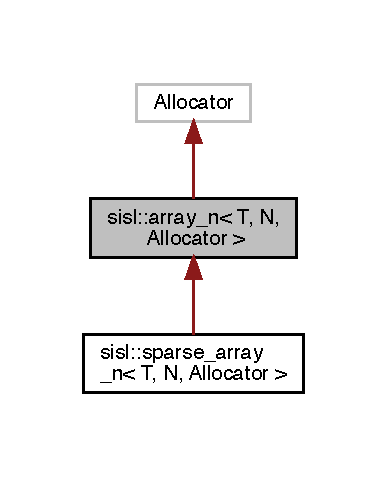
\includegraphics[width=186pt]{classsisl_1_1array__n__inherit__graph}
\end{center}
\end{figure}


Collaboration diagram for sisl\+:\+:array\+\_\+n$<$ T, N, Allocator $>$\+:\nopagebreak
\begin{figure}[H]
\begin{center}
\leavevmode
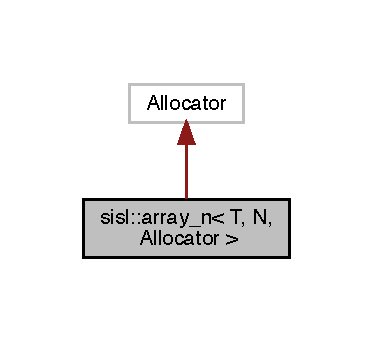
\includegraphics[width=179pt]{classsisl_1_1array__n__coll__graph}
\end{center}
\end{figure}
\subsection*{Public Types}
\begin{DoxyCompactItemize}
\item 
\mbox{\Hypertarget{classsisl_1_1array__n_acb884565621b3575ce99935d0e8bd222}\label{classsisl_1_1array__n_acb884565621b3575ce99935d0e8bd222}} 
typedef T {\bfseries value\+\_\+type}
\item 
\mbox{\Hypertarget{classsisl_1_1array__n_a7093571759e20b2293748a5a72538980}\label{classsisl_1_1array__n_a7093571759e20b2293748a5a72538980}} 
typedef Allocator\+::reference {\bfseries reference}
\item 
\mbox{\Hypertarget{classsisl_1_1array__n_a07b77cbc107044e4797bbbdd31ff01be}\label{classsisl_1_1array__n_a07b77cbc107044e4797bbbdd31ff01be}} 
typedef Allocator\+::const\+\_\+reference {\bfseries const\+\_\+reference}
\item 
\mbox{\Hypertarget{classsisl_1_1array__n_adfa34e632e035525184024e41e6059c2}\label{classsisl_1_1array__n_adfa34e632e035525184024e41e6059c2}} 
typedef Allocator\+::size\+\_\+type {\bfseries size\+\_\+type}
\item 
\mbox{\Hypertarget{classsisl_1_1array__n_a5c6b217f55e5f1f09382b1af6856a4b4}\label{classsisl_1_1array__n_a5c6b217f55e5f1f09382b1af6856a4b4}} 
typedef Allocator\+::difference\+\_\+type {\bfseries difference\+\_\+type}
\item 
\mbox{\Hypertarget{classsisl_1_1array__n_a3de073fb52c6a7ef3d98301edc0c2922}\label{classsisl_1_1array__n_a3de073fb52c6a7ef3d98301edc0c2922}} 
typedef Allocator\+::pointer {\bfseries iterator}
\item 
\mbox{\Hypertarget{classsisl_1_1array__n_a539a2aa750b350a3e8eaeb8a267d8694}\label{classsisl_1_1array__n_a539a2aa750b350a3e8eaeb8a267d8694}} 
typedef Allocator\+::const\+\_\+pointer {\bfseries const\+\_\+iterator}
\item 
\mbox{\Hypertarget{classsisl_1_1array__n_ae665043637f423c1ef474515a129e0b7}\label{classsisl_1_1array__n_ae665043637f423c1ef474515a129e0b7}} 
typedef Allocator {\bfseries allocator\+\_\+type}
\end{DoxyCompactItemize}
\subsection*{Public Member Functions}
\begin{DoxyCompactItemize}
\item 
\mbox{\Hypertarget{classsisl_1_1array__n_a5016fdf6f7a7e6eea1b519b938c3e8c6}\label{classsisl_1_1array__n_a5016fdf6f7a7e6eea1b519b938c3e8c6}} 
allocator\+\_\+type {\bfseries get\+\_\+allocator} () const
\item 
\mbox{\Hypertarget{classsisl_1_1array__n_acf5287e20ac20856d3ce1af561d3d02a}\label{classsisl_1_1array__n_acf5287e20ac20856d3ce1af561d3d02a}} 
\hyperlink{classsisl_1_1array__n_acf5287e20ac20856d3ce1af561d3d02a}{array\+\_\+n} (const Allocator \&a=Allocator())
\begin{DoxyCompactList}\small\item\em Default constructor. Default constructor, allocates nothing. \end{DoxyCompactList}\item 
\mbox{\Hypertarget{classsisl_1_1array__n_ab37d133a8c067cdaf8063ba49205fdea}\label{classsisl_1_1array__n_ab37d133a8c067cdaf8063ba49205fdea}} 
\hyperlink{classsisl_1_1array__n_ab37d133a8c067cdaf8063ba49205fdea}{array\+\_\+n} (const Allocator \&a, unsigned int d0,...)
\begin{DoxyCompactList}\small\item\em N-\/dim constructor. Allocates an array with N dimensions with maximum dimensions given by the parameters. \end{DoxyCompactList}\item 
\mbox{\Hypertarget{classsisl_1_1array__n_a014fd246834441f65441e88d298fc839}\label{classsisl_1_1array__n_a014fd246834441f65441e88d298fc839}} 
\hyperlink{classsisl_1_1array__n_a014fd246834441f65441e88d298fc839}{array\+\_\+n} (unsigned int d0,...)
\begin{DoxyCompactList}\small\item\em N-\/dim constructor. Allocates an array with N dimensions with maximum dimensions given by the parameters. \end{DoxyCompactList}\item 
\mbox{\Hypertarget{classsisl_1_1array__n_a5e645e1a620903d12e4d00f99d58622c}\label{classsisl_1_1array__n_a5e645e1a620903d12e4d00f99d58622c}} 
\hyperlink{classsisl_1_1array__n_a5e645e1a620903d12e4d00f99d58622c}{array\+\_\+n} (const \hyperlink{classsisl_1_1array__n}{array\+\_\+n} \&obj)
\begin{DoxyCompactList}\small\item\em Copy constructor. \end{DoxyCompactList}\item 
\mbox{\Hypertarget{classsisl_1_1array__n_a50e1f1e74ed7f364ea222d56db5a423c}\label{classsisl_1_1array__n_a50e1f1e74ed7f364ea222d56db5a423c}} 
\hyperlink{classsisl_1_1array__n_a50e1f1e74ed7f364ea222d56db5a423c}{$\sim$array\+\_\+n} ()
\begin{DoxyCompactList}\small\item\em Destructor Frees all memory used by this array. \end{DoxyCompactList}\item 
\mbox{\Hypertarget{classsisl_1_1array__n_ae8e89fa53677f239480a7766bc56caf7}\label{classsisl_1_1array__n_ae8e89fa53677f239480a7766bc56caf7}} 
\hyperlink{classsisl_1_1array__n}{array\+\_\+n} \& {\bfseries operator=} (const \hyperlink{classsisl_1_1array__n}{array\+\_\+n} \&obj)
\item 
unsigned int \hyperlink{classsisl_1_1array__n_a89f13ba676e526aa5ed2814514685dc0}{linear\+\_\+index} (unsigned int d0,...) const
\item 
unsigned int \hyperlink{classsisl_1_1array__n_ad10bc825e1ab2bce68b9da0f98be3f1b}{linear\+\_\+index} (unsigned int d0, va\+\_\+list vl) const
\item 
unsigned int \hyperlink{classsisl_1_1array__n_a04888819bc3567f52f52bdccdecd7e5c}{linear\+\_\+index} (unsigned int $\ast$idx) const
\item 
T \& \hyperlink{classsisl_1_1array__n_a1fa1d22e81493e308a6ad66a5100ca43}{operator()} (unsigned int d0,...)
\item 
const T \& \hyperlink{classsisl_1_1array__n_a9630d1014796a2dc2a6fe08f94841115}{operator()} (unsigned int d0,...) const
\item 
T \& \hyperlink{classsisl_1_1array__n_a33e63f670871d57e28133b212b94a0fc}{operator()} (unsigned int $\ast$d)
\item 
const T \& \hyperlink{classsisl_1_1array__n_a6080746c8b0be2377d391b9cc4c8cf4d}{operator()} (unsigned int $\ast$d) const
\item 
\mbox{\Hypertarget{classsisl_1_1array__n_a37afb07dd00ec3770758aca57c5e1f42}\label{classsisl_1_1array__n_a37afb07dd00ec3770758aca57c5e1f42}} 
const bool \hyperlink{classsisl_1_1array__n_a37afb07dd00ec3770758aca57c5e1f42}{has\+\_\+value} (unsigned int d0,...) const
\begin{DoxyCompactList}\small\item\em Returns whether an index has a value For a multidimensional index, this returns whether or not that index has a value. The value at that index will always be readable, use this to know whether or not it\textquotesingle{}s a true value, or an automatically generated value. \end{DoxyCompactList}\item 
\mbox{\Hypertarget{classsisl_1_1array__n_a54507c52f966f7a923a64cb509a09b56}\label{classsisl_1_1array__n_a54507c52f966f7a923a64cb509a09b56}} 
const bool \hyperlink{classsisl_1_1array__n_a54507c52f966f7a923a64cb509a09b56}{has\+\_\+value} (unsigned int $\ast$d) const
\begin{DoxyCompactList}\small\item\em Returns whether an index has a value For a multidimensional index, this returns whether or not that index has a value. The value at that index will always be readable, use this to know whether or not it\textquotesingle{}s a true value, or an automatically generated value. \end{DoxyCompactList}\item 
\mbox{\Hypertarget{classsisl_1_1array__n_a45cb0c98a773ce6e2c4a1315c1cc0a87}\label{classsisl_1_1array__n_a45cb0c98a773ce6e2c4a1315c1cc0a87}} 
bool \hyperlink{classsisl_1_1array__n_a45cb0c98a773ce6e2c4a1315c1cc0a87}{dump\+\_\+to\+\_\+stream} (std\+::ofstream \&stream) const
\begin{DoxyCompactList}\small\item\em Dumps this array to a file stream at its current index. \end{DoxyCompactList}\item 
\mbox{\Hypertarget{classsisl_1_1array__n_abf5a844143174cd0b56d04e82893672d}\label{classsisl_1_1array__n_abf5a844143174cd0b56d04e82893672d}} 
bool \hyperlink{classsisl_1_1array__n_abf5a844143174cd0b56d04e82893672d}{read\+\_\+from\+\_\+stream} (std\+::ifstream \&stream)
\begin{DoxyCompactList}\small\item\em Reads data from a filestream. \end{DoxyCompactList}\end{DoxyCompactItemize}


\subsection{Detailed Description}
\subsubsection*{template$<$class T, int N, class Allocator = std\+::allocator$<$\+T$>$$>$\newline
class sisl\+::array\+\_\+n$<$ T, N, Allocator $>$}

An n-\/dimensional array. This class abstracts away the concept of an n-\/dimensional array, it should be easy to create an array of type T on N dimensions. This is useful as it often ends up being the case that many integer sampling lattices can be broken down into interleaved Cartesian grids. At the end of the day, this implementation flattens the representation down onto dense linear memory. 

However, if your data are sparse, you may benefit from the sparse array class in \hyperlink{sparse__array_8hpp_source}{sparse\+\_\+array.\+hpp} 

\subsection{Member Function Documentation}
\mbox{\Hypertarget{classsisl_1_1array__n_a89f13ba676e526aa5ed2814514685dc0}\label{classsisl_1_1array__n_a89f13ba676e526aa5ed2814514685dc0}} 
\index{sisl\+::array\+\_\+n@{sisl\+::array\+\_\+n}!linear\+\_\+index@{linear\+\_\+index}}
\index{linear\+\_\+index@{linear\+\_\+index}!sisl\+::array\+\_\+n@{sisl\+::array\+\_\+n}}
\subsubsection{\texorpdfstring{linear\+\_\+index()}{linear\_index()}\hspace{0.1cm}{\footnotesize\ttfamily [1/3]}}
{\footnotesize\ttfamily template$<$class T, int N, class Allocator = std\+::allocator$<$\+T$>$$>$ \\
unsigned int \hyperlink{classsisl_1_1array__n}{sisl\+::array\+\_\+n}$<$ T, N, Allocator $>$\+::linear\+\_\+index (\begin{DoxyParamCaption}\item[{unsigned int}]{d0,  }\item[{}]{... }\end{DoxyParamCaption}) const\hspace{0.3cm}{\ttfamily [inline]}}

/brief Returns a unique index for this index. This returns a unique index for a point index, this should generally be an index between 0 and max\+\_\+dim\+\_\+1$\ast$max\+\_\+dim\+\_\+2$\ast$...$\ast$max\+\_\+dim\+\_\+N -\/ 1. \mbox{\Hypertarget{classsisl_1_1array__n_ad10bc825e1ab2bce68b9da0f98be3f1b}\label{classsisl_1_1array__n_ad10bc825e1ab2bce68b9da0f98be3f1b}} 
\index{sisl\+::array\+\_\+n@{sisl\+::array\+\_\+n}!linear\+\_\+index@{linear\+\_\+index}}
\index{linear\+\_\+index@{linear\+\_\+index}!sisl\+::array\+\_\+n@{sisl\+::array\+\_\+n}}
\subsubsection{\texorpdfstring{linear\+\_\+index()}{linear\_index()}\hspace{0.1cm}{\footnotesize\ttfamily [2/3]}}
{\footnotesize\ttfamily template$<$class T, int N, class Allocator = std\+::allocator$<$\+T$>$$>$ \\
unsigned int \hyperlink{classsisl_1_1array__n}{sisl\+::array\+\_\+n}$<$ T, N, Allocator $>$\+::linear\+\_\+index (\begin{DoxyParamCaption}\item[{unsigned int}]{d0,  }\item[{va\+\_\+list}]{vl }\end{DoxyParamCaption}) const\hspace{0.3cm}{\ttfamily [inline]}}

/brief Returns a unique index for this index. This returns a unique index for a point index, this should generally be an index between 0 and max\+\_\+dim\+\_\+1$\ast$max\+\_\+dim\+\_\+2$\ast$...$\ast$max\+\_\+dim\+\_\+N -\/ 1. \mbox{\Hypertarget{classsisl_1_1array__n_a04888819bc3567f52f52bdccdecd7e5c}\label{classsisl_1_1array__n_a04888819bc3567f52f52bdccdecd7e5c}} 
\index{sisl\+::array\+\_\+n@{sisl\+::array\+\_\+n}!linear\+\_\+index@{linear\+\_\+index}}
\index{linear\+\_\+index@{linear\+\_\+index}!sisl\+::array\+\_\+n@{sisl\+::array\+\_\+n}}
\subsubsection{\texorpdfstring{linear\+\_\+index()}{linear\_index()}\hspace{0.1cm}{\footnotesize\ttfamily [3/3]}}
{\footnotesize\ttfamily template$<$class T, int N, class Allocator = std\+::allocator$<$\+T$>$$>$ \\
unsigned int \hyperlink{classsisl_1_1array__n}{sisl\+::array\+\_\+n}$<$ T, N, Allocator $>$\+::linear\+\_\+index (\begin{DoxyParamCaption}\item[{unsigned int $\ast$}]{idx }\end{DoxyParamCaption}) const\hspace{0.3cm}{\ttfamily [inline]}}

/brief Returns a unique index for this index. This returns a unique index for a point index, this should generally be an index between 0 and max\+\_\+dim\+\_\+1$\ast$max\+\_\+dim\+\_\+2$\ast$...$\ast$max\+\_\+dim\+\_\+N -\/ 1. \mbox{\Hypertarget{classsisl_1_1array__n_a1fa1d22e81493e308a6ad66a5100ca43}\label{classsisl_1_1array__n_a1fa1d22e81493e308a6ad66a5100ca43}} 
\index{sisl\+::array\+\_\+n@{sisl\+::array\+\_\+n}!operator()@{operator()}}
\index{operator()@{operator()}!sisl\+::array\+\_\+n@{sisl\+::array\+\_\+n}}
\subsubsection{\texorpdfstring{operator()()}{operator()()}\hspace{0.1cm}{\footnotesize\ttfamily [1/4]}}
{\footnotesize\ttfamily template$<$class T, int N, class Allocator = std\+::allocator$<$\+T$>$$>$ \\
T\& \hyperlink{classsisl_1_1array__n}{sisl\+::array\+\_\+n}$<$ T, N, Allocator $>$\+::operator() (\begin{DoxyParamCaption}\item[{unsigned int}]{d0,  }\item[{}]{... }\end{DoxyParamCaption})\hspace{0.3cm}{\ttfamily [inline]}}

/brief Accessor functions. Access a value in the array, returns a reference so it is possible to write to indices via this overload. \mbox{\Hypertarget{classsisl_1_1array__n_a9630d1014796a2dc2a6fe08f94841115}\label{classsisl_1_1array__n_a9630d1014796a2dc2a6fe08f94841115}} 
\index{sisl\+::array\+\_\+n@{sisl\+::array\+\_\+n}!operator()@{operator()}}
\index{operator()@{operator()}!sisl\+::array\+\_\+n@{sisl\+::array\+\_\+n}}
\subsubsection{\texorpdfstring{operator()()}{operator()()}\hspace{0.1cm}{\footnotesize\ttfamily [2/4]}}
{\footnotesize\ttfamily template$<$class T, int N, class Allocator = std\+::allocator$<$\+T$>$$>$ \\
const T\& \hyperlink{classsisl_1_1array__n}{sisl\+::array\+\_\+n}$<$ T, N, Allocator $>$\+::operator() (\begin{DoxyParamCaption}\item[{unsigned int}]{d0,  }\item[{}]{... }\end{DoxyParamCaption}) const\hspace{0.3cm}{\ttfamily [inline]}}

/brief Accessor functions. Access a value in the array, returns a reference so it is possible to write to indices via this overload. \mbox{\Hypertarget{classsisl_1_1array__n_a33e63f670871d57e28133b212b94a0fc}\label{classsisl_1_1array__n_a33e63f670871d57e28133b212b94a0fc}} 
\index{sisl\+::array\+\_\+n@{sisl\+::array\+\_\+n}!operator()@{operator()}}
\index{operator()@{operator()}!sisl\+::array\+\_\+n@{sisl\+::array\+\_\+n}}
\subsubsection{\texorpdfstring{operator()()}{operator()()}\hspace{0.1cm}{\footnotesize\ttfamily [3/4]}}
{\footnotesize\ttfamily template$<$class T, int N, class Allocator = std\+::allocator$<$\+T$>$$>$ \\
T\& \hyperlink{classsisl_1_1array__n}{sisl\+::array\+\_\+n}$<$ T, N, Allocator $>$\+::operator() (\begin{DoxyParamCaption}\item[{unsigned int $\ast$}]{d }\end{DoxyParamCaption})\hspace{0.3cm}{\ttfamily [inline]}}

/brief Accessor functions. Access a value in the array, returns a reference so it is possible to write to indices via this overload. \mbox{\Hypertarget{classsisl_1_1array__n_a6080746c8b0be2377d391b9cc4c8cf4d}\label{classsisl_1_1array__n_a6080746c8b0be2377d391b9cc4c8cf4d}} 
\index{sisl\+::array\+\_\+n@{sisl\+::array\+\_\+n}!operator()@{operator()}}
\index{operator()@{operator()}!sisl\+::array\+\_\+n@{sisl\+::array\+\_\+n}}
\subsubsection{\texorpdfstring{operator()()}{operator()()}\hspace{0.1cm}{\footnotesize\ttfamily [4/4]}}
{\footnotesize\ttfamily template$<$class T, int N, class Allocator = std\+::allocator$<$\+T$>$$>$ \\
const T\& \hyperlink{classsisl_1_1array__n}{sisl\+::array\+\_\+n}$<$ T, N, Allocator $>$\+::operator() (\begin{DoxyParamCaption}\item[{unsigned int $\ast$}]{d }\end{DoxyParamCaption}) const\hspace{0.3cm}{\ttfamily [inline]}}

/brief Accessor functions. Access a value in the array, returns a reference so it is possible to write to indices via this overload. 

The documentation for this class was generated from the following file\+:\begin{DoxyCompactItemize}
\item 
/\+Users/joshuahoracsek/\+Projects/sisl\+\_\+redux/include/sisl/memory/array.\+hpp\end{DoxyCompactItemize}

\hypertarget{classsisl_1_1base__lattice}{}\section{sisl\+:\+:base\+\_\+lattice$<$ T $>$ Class Template Reference}
\label{classsisl_1_1base__lattice}\index{sisl\+::base\+\_\+lattice$<$ T $>$@{sisl\+::base\+\_\+lattice$<$ T $>$}}


Base abstract lattice class. Defines the base class for a lattice, which are by definition subsets of Z$^\wedge$n.  




{\ttfamily \#include $<$base\+\_\+lattice.\+hpp$>$}



Inheritance diagram for sisl\+:\+:base\+\_\+lattice$<$ T $>$\+:\nopagebreak
\begin{figure}[H]
\begin{center}
\leavevmode
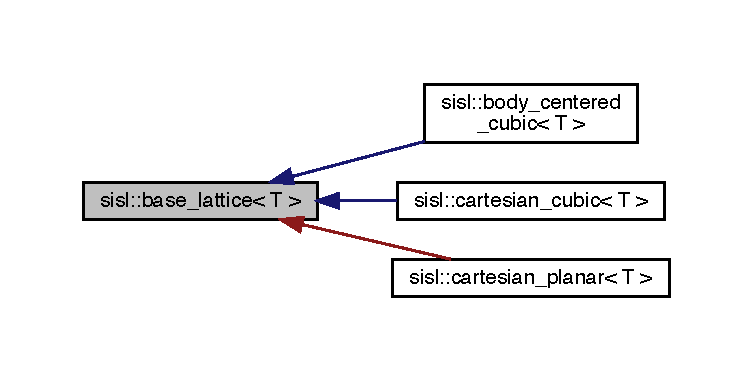
\includegraphics[width=350pt]{classsisl_1_1base__lattice__inherit__graph}
\end{center}
\end{figure}
\subsection*{Public Member Functions}
\begin{DoxyCompactItemize}
\item 
\mbox{\Hypertarget{classsisl_1_1base__lattice_a45737aef697099b47f539a6084c81a15}\label{classsisl_1_1base__lattice_a45737aef697099b47f539a6084c81a15}} 
virtual T \& \hyperlink{classsisl_1_1base__lattice_a45737aef697099b47f539a6084c81a15}{operator()} (int d0,...)=0
\begin{DoxyCompactList}\small\item\em Access a lattice site. Operators for accessing lattice sites. These index in the natural coordinate system of the lattice. \end{DoxyCompactList}\item 
\mbox{\Hypertarget{classsisl_1_1base__lattice_ad2193e17c508f1f476164a4494ecba87}\label{classsisl_1_1base__lattice_ad2193e17c508f1f476164a4494ecba87}} 
virtual const T \& \hyperlink{classsisl_1_1base__lattice_ad2193e17c508f1f476164a4494ecba87}{operator()} (int d0,...) const =0
\begin{DoxyCompactList}\small\item\em Access a lattice site. Operators for accessing lattice sites. These index in the natural coordinate system of the lattice. \end{DoxyCompactList}\item 
\mbox{\Hypertarget{classsisl_1_1base__lattice_ac95ec229ba562861dbfd7c43130e3d5f}\label{classsisl_1_1base__lattice_ac95ec229ba562861dbfd7c43130e3d5f}} 
virtual T \& \hyperlink{classsisl_1_1base__lattice_ac95ec229ba562861dbfd7c43130e3d5f}{operator()} (int $\ast$d)=0
\begin{DoxyCompactList}\small\item\em Access a lattice site. Operators for accessing lattice sites. These index in the natural coordinate system of the lattice. \end{DoxyCompactList}\item 
\mbox{\Hypertarget{classsisl_1_1base__lattice_a51e4e2d9717669822dc797b05742db48}\label{classsisl_1_1base__lattice_a51e4e2d9717669822dc797b05742db48}} 
virtual const T \& \hyperlink{classsisl_1_1base__lattice_a51e4e2d9717669822dc797b05742db48}{operator()} (int $\ast$d) const =0
\begin{DoxyCompactList}\small\item\em Access a lattice site. Operators for accessing lattice sites. These index in the natural coordinate system of the lattice. \end{DoxyCompactList}\item 
\mbox{\Hypertarget{classsisl_1_1base__lattice_a4b1b4b0ebdea39182f1962a020ce1dba}\label{classsisl_1_1base__lattice_a4b1b4b0ebdea39182f1962a020ce1dba}} 
virtual T \& \hyperlink{classsisl_1_1base__lattice_a4b1b4b0ebdea39182f1962a020ce1dba}{operator()} (const \hyperlink{namespacesisl_acd18feee4026583db6185df2b25434aa}{lattice\+\_\+site} \&s)=0
\begin{DoxyCompactList}\small\item\em Access a lattice site. Operators for accessing lattice sites. These index in the natural coordinate system of the lattice. \end{DoxyCompactList}\item 
\mbox{\Hypertarget{classsisl_1_1base__lattice_ad522b89ea83ddd5fdead55d51a3e7432}\label{classsisl_1_1base__lattice_ad522b89ea83ddd5fdead55d51a3e7432}} 
virtual const T \& \hyperlink{classsisl_1_1base__lattice_ad522b89ea83ddd5fdead55d51a3e7432}{operator()} (const \hyperlink{namespacesisl_acd18feee4026583db6185df2b25434aa}{lattice\+\_\+site} \&s) const =0
\begin{DoxyCompactList}\small\item\em Access a lattice site. Operators for accessing lattice sites. These index in the natural coordinate system of the lattice. \end{DoxyCompactList}\item 
\mbox{\Hypertarget{classsisl_1_1base__lattice_a75869d632df9aba88b0a8ff289950d23}\label{classsisl_1_1base__lattice_a75869d632df9aba88b0a8ff289950d23}} 
virtual const unsigned int \hyperlink{classsisl_1_1base__lattice_a75869d632df9aba88b0a8ff289950d23}{linear\+\_\+index} (int d0,...) const =0
\begin{DoxyCompactList}\small\item\em Uniquely index a lattice site This function return a linearized version of a lattice site, this allows one to uniquely associate a lattice site with an integer. \end{DoxyCompactList}\item 
\mbox{\Hypertarget{classsisl_1_1base__lattice_abacb50c47e6b1b790b9ae4130c219818}\label{classsisl_1_1base__lattice_abacb50c47e6b1b790b9ae4130c219818}} 
virtual const unsigned int \hyperlink{classsisl_1_1base__lattice_abacb50c47e6b1b790b9ae4130c219818}{linear\+\_\+index} (int $\ast$d) const =0
\begin{DoxyCompactList}\small\item\em Uniquely index a lattice site This function return a linearized version of a lattice site, this allows one to uniquely associate a lattice site with an integer. \end{DoxyCompactList}\item 
\mbox{\Hypertarget{classsisl_1_1base__lattice_af773eb97992177cc5249cf951f9daa40}\label{classsisl_1_1base__lattice_af773eb97992177cc5249cf951f9daa40}} 
virtual const unsigned int \hyperlink{classsisl_1_1base__lattice_af773eb97992177cc5249cf951f9daa40}{linear\+\_\+index} (const \hyperlink{namespacesisl_acd18feee4026583db6185df2b25434aa}{lattice\+\_\+site} \&) const =0
\begin{DoxyCompactList}\small\item\em Uniquely index a lattice site This function return a linearized version of a lattice site, this allows one to uniquely associate a lattice site with an integer. \end{DoxyCompactList}\item 
\mbox{\Hypertarget{classsisl_1_1base__lattice_a832e11c4873b26282d1061986096ca48}\label{classsisl_1_1base__lattice_a832e11c4873b26282d1061986096ca48}} 
virtual const \hyperlink{namespacesisl_a2069bd5374a9be042ff3ce3306d41e1a}{vector} \hyperlink{classsisl_1_1base__lattice_a832e11c4873b26282d1061986096ca48}{get\+\_\+natural\+\_\+scales} () const =0
\begin{DoxyCompactList}\small\item\em Returns a natural scale so that the lattice sites would be scaled to within a unit hyper cube. \end{DoxyCompactList}\item 
\mbox{\Hypertarget{classsisl_1_1base__lattice_abac229515b996da70ebe94773fc6f941}\label{classsisl_1_1base__lattice_abac229515b996da70ebe94773fc6f941}} 
virtual const \hyperlink{namespacesisl_acd18feee4026583db6185df2b25434aa}{lattice\+\_\+site} \hyperlink{classsisl_1_1base__lattice_abac229515b996da70ebe94773fc6f941}{get\+\_\+dimensions} () const =0
\begin{DoxyCompactList}\small\item\em Returns the integer extent of each dimension, that is, the lattice extends from \mbox{[}0, ret\mbox{[}i\mbox{]} -\/ 1\mbox{]} in each dimension. \end{DoxyCompactList}\item 
\mbox{\Hypertarget{classsisl_1_1base__lattice_a51a87e1f121f2345f8f6882a29b62f38}\label{classsisl_1_1base__lattice_a51a87e1f121f2345f8f6882a29b62f38}} 
virtual \hyperlink{namespacesisl_a2069bd5374a9be042ff3ce3306d41e1a}{vector} \hyperlink{classsisl_1_1base__lattice_a51a87e1f121f2345f8f6882a29b62f38}{get\+\_\+site\+\_\+position} (int d0,...) const =0
\begin{DoxyCompactList}\small\item\em Returns a value within the unit hyper cube that represents the given lattice site scaled withing that unit hypercube. \end{DoxyCompactList}\item 
\mbox{\Hypertarget{classsisl_1_1base__lattice_a25f87033a3974fff880f124c49c3dbe3}\label{classsisl_1_1base__lattice_a25f87033a3974fff880f124c49c3dbe3}} 
virtual \hyperlink{namespacesisl_a2069bd5374a9be042ff3ce3306d41e1a}{vector} \hyperlink{classsisl_1_1base__lattice_a25f87033a3974fff880f124c49c3dbe3}{get\+\_\+site\+\_\+position} (int $\ast$d) const =0
\begin{DoxyCompactList}\small\item\em Returns a value within the unit hyper cube that represents the given lattice site scaled withing that unit hypercube. \end{DoxyCompactList}\item 
\mbox{\Hypertarget{classsisl_1_1base__lattice_a030d1230d44e9c88e8f79ef87920b4ed}\label{classsisl_1_1base__lattice_a030d1230d44e9c88e8f79ef87920b4ed}} 
virtual \hyperlink{namespacesisl_a2069bd5374a9be042ff3ce3306d41e1a}{vector} \hyperlink{classsisl_1_1base__lattice_a030d1230d44e9c88e8f79ef87920b4ed}{get\+\_\+site\+\_\+position} (const \hyperlink{namespacesisl_acd18feee4026583db6185df2b25434aa}{lattice\+\_\+site} \&s) const =0
\begin{DoxyCompactList}\small\item\em Returns a value within the unit hyper cube that represents the given lattice site scaled withing that unit hypercube. \end{DoxyCompactList}\item 
\mbox{\Hypertarget{classsisl_1_1base__lattice_a0b789f66f4b822a62b2d5b22fa2804b5}\label{classsisl_1_1base__lattice_a0b789f66f4b822a62b2d5b22fa2804b5}} 
virtual \hyperlink{namespacesisl_acd18feee4026583db6185df2b25434aa}{lattice\+\_\+site} \hyperlink{classsisl_1_1base__lattice_a0b789f66f4b822a62b2d5b22fa2804b5}{get\+\_\+nearest\+\_\+site} (const \hyperlink{namespacesisl_a2069bd5374a9be042ff3ce3306d41e1a}{vector} \&) const =0
\begin{DoxyCompactList}\small\item\em Returns the nearest lattice site for a given point within the unit hyper cube. \end{DoxyCompactList}\item 
\mbox{\Hypertarget{classsisl_1_1base__lattice_a4db34d7dc53ec4358433218a7daf33f9}\label{classsisl_1_1base__lattice_a4db34d7dc53ec4358433218a7daf33f9}} 
virtual bool \hyperlink{classsisl_1_1base__lattice_a4db34d7dc53ec4358433218a7daf33f9}{is\+\_\+lattice\+\_\+site} (int d0,...) const =0
\begin{DoxyCompactList}\small\item\em Returns whether or not a lattice site truely corresponds to a valid lattice site on this particular lattice. \end{DoxyCompactList}\item 
\mbox{\Hypertarget{classsisl_1_1base__lattice_affd433798fb68d45b7265c0bd5e9e1ac}\label{classsisl_1_1base__lattice_affd433798fb68d45b7265c0bd5e9e1ac}} 
virtual bool \hyperlink{classsisl_1_1base__lattice_affd433798fb68d45b7265c0bd5e9e1ac}{is\+\_\+lattice\+\_\+site} (int $\ast$d) const =0
\begin{DoxyCompactList}\small\item\em Returns whether or not a lattice site truely corresponds to a valid lattice site on this particular lattice. \end{DoxyCompactList}\item 
\mbox{\Hypertarget{classsisl_1_1base__lattice_aae9dc75c53a39031e2c8a5a4b9ce6855}\label{classsisl_1_1base__lattice_aae9dc75c53a39031e2c8a5a4b9ce6855}} 
virtual bool \hyperlink{classsisl_1_1base__lattice_aae9dc75c53a39031e2c8a5a4b9ce6855}{is\+\_\+lattice\+\_\+site} (const \hyperlink{namespacesisl_acd18feee4026583db6185df2b25434aa}{lattice\+\_\+site} \&) const =0
\begin{DoxyCompactList}\small\item\em Returns whether or not a lattice\+\_\+site object truely corresponds to a valid lattice site on this particular lattice. \end{DoxyCompactList}\item 
\mbox{\Hypertarget{classsisl_1_1base__lattice_a2a1746ce0ea77eb219a1667e88502fe4}\label{classsisl_1_1base__lattice_a2a1746ce0ea77eb219a1667e88502fe4}} 
virtual bool \hyperlink{classsisl_1_1base__lattice_a2a1746ce0ea77eb219a1667e88502fe4}{is\+\_\+filled} (int d0,...) const =0
\begin{DoxyCompactList}\small\item\em Returns whether a lattice site actually contains a value. \end{DoxyCompactList}\item 
\mbox{\Hypertarget{classsisl_1_1base__lattice_aa58f16669b8cc44aeaa71a87243e588d}\label{classsisl_1_1base__lattice_aa58f16669b8cc44aeaa71a87243e588d}} 
virtual bool \hyperlink{classsisl_1_1base__lattice_aa58f16669b8cc44aeaa71a87243e588d}{is\+\_\+filled} (int $\ast$d) const =0
\begin{DoxyCompactList}\small\item\em Returns whether a lattice site actually contains a value. \end{DoxyCompactList}\item 
\mbox{\Hypertarget{classsisl_1_1base__lattice_a883cb05212eb7339bd73dd8ddf8968ca}\label{classsisl_1_1base__lattice_a883cb05212eb7339bd73dd8ddf8968ca}} 
virtual bool \hyperlink{classsisl_1_1base__lattice_a883cb05212eb7339bd73dd8ddf8968ca}{is\+\_\+filled} (const \hyperlink{namespacesisl_acd18feee4026583db6185df2b25434aa}{lattice\+\_\+site} \&s) const =0
\begin{DoxyCompactList}\small\item\em Returns whether a lattice site actually contains a value. \end{DoxyCompactList}\item 
\mbox{\Hypertarget{classsisl_1_1base__lattice_a3ff5b00f3d8c41e59672e6fa76456ff9}\label{classsisl_1_1base__lattice_a3ff5b00f3d8c41e59672e6fa76456ff9}} 
virtual void \hyperlink{classsisl_1_1base__lattice_a3ff5b00f3d8c41e59672e6fa76456ff9}{each\+\_\+site} (const std\+::function$<$ void(const \hyperlink{namespacesisl_acd18feee4026583db6185df2b25434aa}{lattice\+\_\+site} \&)$>$ \&, bool parallel=false)=0
\begin{DoxyCompactList}\small\item\em Iterates over every lattice site contained within the dimensions of this lattice. \end{DoxyCompactList}\item 
\mbox{\Hypertarget{classsisl_1_1base__lattice_a663d4e3b07c524970848377b66de9425}\label{classsisl_1_1base__lattice_a663d4e3b07c524970848377b66de9425}} 
virtual std\+::string \hyperlink{classsisl_1_1base__lattice_a663d4e3b07c524970848377b66de9425}{get\+\_\+lattice\+\_\+name} () const =0
\begin{DoxyCompactList}\small\item\em Returns the name of this lattice. \end{DoxyCompactList}\item 
\mbox{\Hypertarget{classsisl_1_1base__lattice_a57946d77d273c39cffba678241f4f8d3}\label{classsisl_1_1base__lattice_a57946d77d273c39cffba678241f4f8d3}} 
virtual const int \hyperlink{classsisl_1_1base__lattice_a57946d77d273c39cffba678241f4f8d3}{number\+\_\+of\+\_\+lattice\+\_\+sites} () const =0
\begin{DoxyCompactList}\small\item\em Returns the theoretical number of sites within this lattice. \end{DoxyCompactList}\item 
\mbox{\Hypertarget{classsisl_1_1base__lattice_a78cf60c535a188fd07bbd4ae4379b7bd}\label{classsisl_1_1base__lattice_a78cf60c535a188fd07bbd4ae4379b7bd}} 
virtual bool \hyperlink{classsisl_1_1base__lattice_a78cf60c535a188fd07bbd4ae4379b7bd}{dump\+\_\+to\+\_\+stream} (std\+::ofstream \&) const =0
\begin{DoxyCompactList}\small\item\em Dumps this lattice to a file stream. \end{DoxyCompactList}\item 
\mbox{\Hypertarget{classsisl_1_1base__lattice_ad81c46a32112789f61bcab1e090ec95d}\label{classsisl_1_1base__lattice_ad81c46a32112789f61bcab1e090ec95d}} 
virtual bool \hyperlink{classsisl_1_1base__lattice_ad81c46a32112789f61bcab1e090ec95d}{read\+\_\+from\+\_\+stream} (std\+::ifstream \&)=0
\begin{DoxyCompactList}\small\item\em Reads a lattice to a file stream, replacing all values. \end{DoxyCompactList}\item 
\mbox{\Hypertarget{classsisl_1_1base__lattice_ac19afb43147c6c4443123b982af3417d}\label{classsisl_1_1base__lattice_ac19afb43147c6c4443123b982af3417d}} 
virtual void \hyperlink{classsisl_1_1base__lattice_ac19afb43147c6c4443123b982af3417d}{set\+\_\+extension\+\_\+type} (const \hyperlink{namespacesisl_aaf1f41d23ed37dacaa4c9f1bb6d3324f}{Lattice\+Extension\+Type} \&e, const \hyperlink{namespacesisl_af139f6f74488292ae48c0d71eaa5d4f1}{Lattice\+Region\+Shift} \&s)=0
\begin{DoxyCompactList}\small\item\em Sets how a lattice is extended for values that outside of the defined rectangular region. \end{DoxyCompactList}\end{DoxyCompactItemize}
\subsection*{Protected Member Functions}
\begin{DoxyCompactItemize}
\item 
\mbox{\Hypertarget{classsisl_1_1base__lattice_ab04b5358fb717e4f14a7ba8d4c65ebf0}\label{classsisl_1_1base__lattice_ab04b5358fb717e4f14a7ba8d4c65ebf0}} 
virtual const unsigned int {\bfseries linear\+\_\+index} (int d0, va\+\_\+list vl) const =0
\item 
\mbox{\Hypertarget{classsisl_1_1base__lattice_af588d28f96cd42b92bf0d8f81170899d}\label{classsisl_1_1base__lattice_af588d28f96cd42b92bf0d8f81170899d}} 
virtual T \& {\bfseries operator()} (int d0, va\+\_\+list vl)=0
\item 
\mbox{\Hypertarget{classsisl_1_1base__lattice_a15fc29455feb062e995773f7dc728114}\label{classsisl_1_1base__lattice_a15fc29455feb062e995773f7dc728114}} 
virtual const T \& {\bfseries operator()} (int d0, va\+\_\+list vl) const =0
\item 
\mbox{\Hypertarget{classsisl_1_1base__lattice_a7cc857d33e9d15d6ee85d47821d7ab3b}\label{classsisl_1_1base__lattice_a7cc857d33e9d15d6ee85d47821d7ab3b}} 
virtual bool {\bfseries is\+\_\+filled} (int d0, va\+\_\+list vl) const =0
\item 
\mbox{\Hypertarget{classsisl_1_1base__lattice_a64b9bca3305602a1613c8732a4cdb74f}\label{classsisl_1_1base__lattice_a64b9bca3305602a1613c8732a4cdb74f}} 
virtual bool {\bfseries is\+\_\+lattice\+\_\+site} (int d0, va\+\_\+list vl) const =0
\end{DoxyCompactItemize}


\subsection{Detailed Description}
\subsubsection*{template$<$class T$>$\newline
class sisl\+::base\+\_\+lattice$<$ T $>$}

Base abstract lattice class. Defines the base class for a lattice, which are by definition subsets of Z$^\wedge$n. 

The documentation for this class was generated from the following file\+:\begin{DoxyCompactItemize}
\item 
/\+Users/joshuahoracsek/\+Projects/sisl\+\_\+redux/include/sisl/lattice/base\+\_\+lattice.\+hpp\end{DoxyCompactItemize}

\hypertarget{classsisl_1_1basis__function}{}\section{sisl\+:\+:basis\+\_\+function Class Reference}
\label{classsisl_1_1basis__function}\index{sisl\+::basis\+\_\+function@{sisl\+::basis\+\_\+function}}


Abstract definition of a basis function. Provides an interface that any basis function of a shift invariant space must adhere to. This also provides the heavy lifting code for a ``brute force\textquotesingle{}\textquotesingle{} convolution sum. \hyperlink{classsisl_1_1tp__linear}{tp\+\_\+linear} is a good example of how to implement basis functions.  




{\ttfamily \#include $<$basis\+\_\+function.\+hpp$>$}



Inheritance diagram for sisl\+:\+:basis\+\_\+function\+:\nopagebreak
\begin{figure}[H]
\begin{center}
\leavevmode
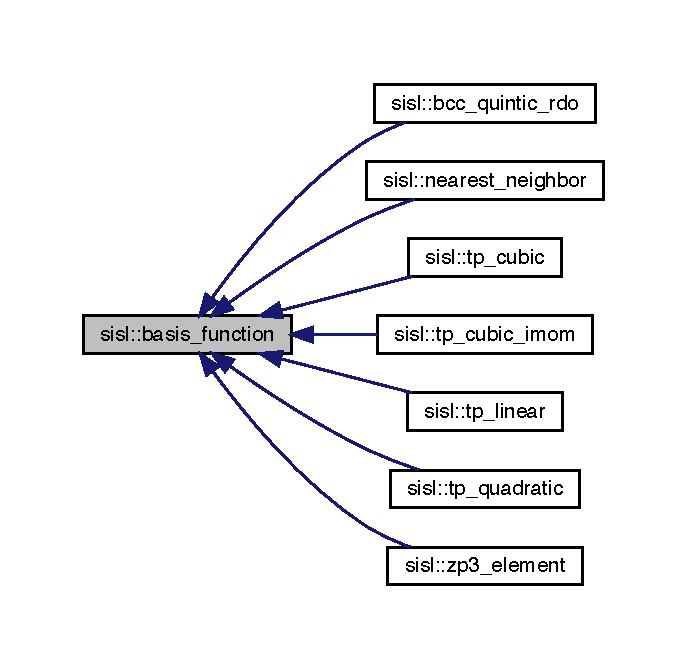
\includegraphics[width=330pt]{classsisl_1_1basis__function__inherit__graph}
\end{center}
\end{figure}
\subsection*{Static Public Member Functions}
\begin{DoxyCompactItemize}
\item 
\mbox{\Hypertarget{classsisl_1_1basis__function_ae263cdbf1ad31e828d43af62fd645d6d}\label{classsisl_1_1basis__function_ae263cdbf1ad31e828d43af62fd645d6d}} 
{\footnotesize template$<$int N$>$ }\\static const double \hyperlink{classsisl_1_1basis__function_ae263cdbf1ad31e828d43af62fd645d6d}{phi} (const \hyperlink{namespacesisl_a2069bd5374a9be042ff3ce3306d41e1a}{vector} \&p)
\begin{DoxyCompactList}\small\item\em Evaluates the un-\/scaled basis function. Evaluates the basis function as if it were not scaled by any scaling parameter. \end{DoxyCompactList}\item 
\mbox{\Hypertarget{classsisl_1_1basis__function_a5a0fc716cb31c0b4a39ae9ffef9210dd}\label{classsisl_1_1basis__function_a5a0fc716cb31c0b4a39ae9ffef9210dd}} 
{\footnotesize template$<$int N$>$ }\\static const double \hyperlink{classsisl_1_1basis__function_a5a0fc716cb31c0b4a39ae9ffef9210dd}{phi} (const double \&h, const \hyperlink{namespacesisl_a2069bd5374a9be042ff3ce3306d41e1a}{vector} \&p)
\begin{DoxyCompactList}\small\item\em Evaluates the un-\/scaled basis function. Evaluates the basis function as if it were not scaled by any scaling parameter. This, however, does take a scale parameter, as the basis may change per scale (e.\+g. exponential splines) \end{DoxyCompactList}\item 
\mbox{\Hypertarget{classsisl_1_1basis__function_a08ca4f754c0f9bd937f362c91b37a159}\label{classsisl_1_1basis__function_a08ca4f754c0f9bd937f362c91b37a159}} 
{\footnotesize template$<$int N$>$ }\\static const double \hyperlink{classsisl_1_1basis__function_a08ca4f754c0f9bd937f362c91b37a159}{dphi} (const \hyperlink{namespacesisl_a2069bd5374a9be042ff3ce3306d41e1a}{vector} \&p, const int \&d)
\begin{DoxyCompactList}\small\item\em Evaluates the derivative of an un-\/scaled basis function. Evaluates the derivative of a basis function as if it were not scaled by any scaling parameter. \end{DoxyCompactList}\item 
\mbox{\Hypertarget{classsisl_1_1basis__function_ad4210a18404d763b781152fb41b3f173}\label{classsisl_1_1basis__function_ad4210a18404d763b781152fb41b3f173}} 
{\footnotesize template$<$int N$>$ }\\static const double \hyperlink{classsisl_1_1basis__function_ad4210a18404d763b781152fb41b3f173}{dphi} (const double \&h, const \hyperlink{namespacesisl_a2069bd5374a9be042ff3ce3306d41e1a}{vector} \&p, const int \&d)
\begin{DoxyCompactList}\small\item\em Evaluates the derivative of the un-\/scaled basis function. Evaluates the basis function as if it were not scaled by any scaling parameter. This, however, does take a scale parameter, as the basis may change per scale (e.\+g. exponential splines) \end{DoxyCompactList}\item 
\mbox{\Hypertarget{classsisl_1_1basis__function_a6e8b07cacc2f6a14272992d40c19cabb}\label{classsisl_1_1basis__function_a6e8b07cacc2f6a14272992d40c19cabb}} 
{\footnotesize template$<$int N$>$ }\\static std\+::vector$<$ \hyperlink{namespacesisl_acd18feee4026583db6185df2b25434aa}{lattice\+\_\+site} $>$ \hyperlink{classsisl_1_1basis__function_a6e8b07cacc2f6a14272992d40c19cabb}{get\+\_\+integer\+\_\+support} ()
\begin{DoxyCompactList}\small\item\em Returns the integer support for this basis function. Returns the closure of the support of the basis function, intersected with the integer lattice. \end{DoxyCompactList}\item 
\mbox{\Hypertarget{classsisl_1_1basis__function_a320a0e4a41913993312fa99e59605663}\label{classsisl_1_1basis__function_a320a0e4a41913993312fa99e59605663}} 
static bool {\bfseries has\+\_\+derivative} ()
\item 
\mbox{\Hypertarget{classsisl_1_1basis__function_acbd2e8d5399260b958bb781685b38983}\label{classsisl_1_1basis__function_acbd2e8d5399260b958bb781685b38983}} 
{\footnotesize template$<$int N, class L , class BF $>$ }\\static double {\bfseries convolution\+\_\+sum} (const \hyperlink{namespacesisl_a2069bd5374a9be042ff3ce3306d41e1a}{vector} \&p, const L $\ast$lattice)
\item 
\mbox{\Hypertarget{classsisl_1_1basis__function_acd7a5e4de21481e6a543fa65f92c19c9}\label{classsisl_1_1basis__function_acd7a5e4de21481e6a543fa65f92c19c9}} 
{\footnotesize template$<$int N, class L , class BF $>$ }\\static double {\bfseries convolution\+\_\+sum\+\_\+deriv} (const \hyperlink{namespacesisl_a2069bd5374a9be042ff3ce3306d41e1a}{vector} \&p, const L $\ast$lattice, const int \&component)
\item 
\mbox{\Hypertarget{classsisl_1_1basis__function_afacf657c3306f83ae42d73978ee38a47}\label{classsisl_1_1basis__function_afacf657c3306f83ae42d73978ee38a47}} 
{\footnotesize template$<$int N, class L , class BF $>$ }\\static \hyperlink{namespacesisl_a2069bd5374a9be042ff3ce3306d41e1a}{vector} {\bfseries grad\+\_\+convolution\+\_\+sum} (const \hyperlink{namespacesisl_a2069bd5374a9be042ff3ce3306d41e1a}{vector} \&p, const L $\ast$lattice)
\item 
\mbox{\Hypertarget{classsisl_1_1basis__function_ae4e59e60ccac8d4060a417f9f0353d53}\label{classsisl_1_1basis__function_ae4e59e60ccac8d4060a417f9f0353d53}} 
{\footnotesize template$<$int N, class L , class BF $>$ }\\static \hyperlink{namespacesisl_a2069bd5374a9be042ff3ce3306d41e1a}{vector} {\bfseries grad\+\_\+convolution\+\_\+sum} (const \hyperlink{namespacesisl_a2069bd5374a9be042ff3ce3306d41e1a}{vector} \&p, const L $\ast$base, const L $\ast$$\ast$lattices)
\item 
\mbox{\Hypertarget{classsisl_1_1basis__function_aa7171cdb11702fcc6bfe49de1925a1a4}\label{classsisl_1_1basis__function_aa7171cdb11702fcc6bfe49de1925a1a4}} 
{\footnotesize template$<$int N, class L , class BF $>$ }\\static double {\bfseries convolution\+\_\+sum\+\_\+h} (const \hyperlink{namespacesisl_a2069bd5374a9be042ff3ce3306d41e1a}{vector} \&p, const L $\ast$lattice, const double \&h)
\item 
\mbox{\Hypertarget{classsisl_1_1basis__function_a1bed96cde85d879444b965f7d3c9199d}\label{classsisl_1_1basis__function_a1bed96cde85d879444b965f7d3c9199d}} 
{\footnotesize template$<$int N, class L , class BF $>$ }\\static double {\bfseries convolution\+\_\+sum\+\_\+deriv\+\_\+h} (const \hyperlink{namespacesisl_a2069bd5374a9be042ff3ce3306d41e1a}{vector} \&p, const L $\ast$lattice, const int \&component, const double \&h)
\item 
\mbox{\Hypertarget{classsisl_1_1basis__function_a5e9afa1d8e02b37de4fc6d38fcf79b56}\label{classsisl_1_1basis__function_a5e9afa1d8e02b37de4fc6d38fcf79b56}} 
{\footnotesize template$<$int N, class L , class BF $>$ }\\static \hyperlink{namespacesisl_a2069bd5374a9be042ff3ce3306d41e1a}{vector} {\bfseries grad\+\_\+convolution\+\_\+sum\+\_\+h} (const \hyperlink{namespacesisl_a2069bd5374a9be042ff3ce3306d41e1a}{vector} \&p, const L $\ast$lattice, const double \&h)
\item 
\mbox{\Hypertarget{classsisl_1_1basis__function_aaee0095420132eb4a2b798c3ec135ce9}\label{classsisl_1_1basis__function_aaee0095420132eb4a2b798c3ec135ce9}} 
{\footnotesize template$<$int N, class L , class BF $>$ }\\static \hyperlink{namespacesisl_a2069bd5374a9be042ff3ce3306d41e1a}{vector} {\bfseries grad\+\_\+convolution\+\_\+sum\+\_\+h} (const \hyperlink{namespacesisl_a2069bd5374a9be042ff3ce3306d41e1a}{vector} \&p, const L $\ast$base, const L $\ast$$\ast$lattices, const double \&h)
\end{DoxyCompactItemize}


\subsection{Detailed Description}
Abstract definition of a basis function. Provides an interface that any basis function of a shift invariant space must adhere to. This also provides the heavy lifting code for a ``brute force\textquotesingle{}\textquotesingle{} convolution sum. \hyperlink{classsisl_1_1tp__linear}{tp\+\_\+linear} is a good example of how to implement basis functions. 

The documentation for this class was generated from the following file\+:\begin{DoxyCompactItemize}
\item 
/\+Users/joshuahoracsek/\+Projects/sisl\+\_\+redux/include/sisl/basis/basis\+\_\+function.\+hpp\end{DoxyCompactItemize}

\hypertarget{classsisl_1_1bcc__quintic__rdo}{}\section{sisl\+:\+:bcc\+\_\+quintic\+\_\+rdo Class Reference}
\label{classsisl_1_1bcc__quintic__rdo}\index{sisl\+::bcc\+\_\+quintic\+\_\+rdo@{sisl\+::bcc\+\_\+quintic\+\_\+rdo}}


Quintic B\+CC basis function.  




{\ttfamily \#include $<$quintic\+\_\+rdo.\+hpp$>$}



Inheritance diagram for sisl\+:\+:bcc\+\_\+quintic\+\_\+rdo\+:\nopagebreak
\begin{figure}[H]
\begin{center}
\leavevmode
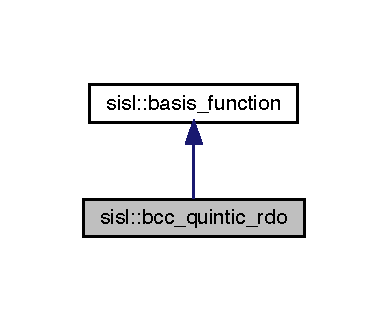
\includegraphics[width=186pt]{classsisl_1_1bcc__quintic__rdo__inherit__graph}
\end{center}
\end{figure}


Collaboration diagram for sisl\+:\+:bcc\+\_\+quintic\+\_\+rdo\+:\nopagebreak
\begin{figure}[H]
\begin{center}
\leavevmode
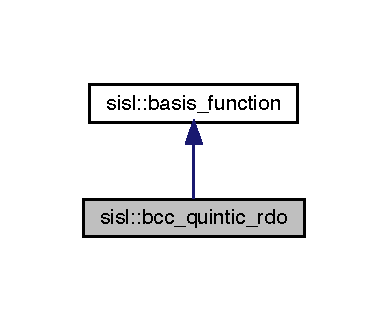
\includegraphics[width=186pt]{classsisl_1_1bcc__quintic__rdo__coll__graph}
\end{center}
\end{figure}
\subsection*{Static Public Member Functions}
\begin{DoxyCompactItemize}
\item 
\mbox{\Hypertarget{classsisl_1_1bcc__quintic__rdo_af269427e5d0bc33a12310befac01d1d4}\label{classsisl_1_1bcc__quintic__rdo_af269427e5d0bc33a12310befac01d1d4}} 
{\footnotesize template$<$int N$>$ }\\static const double {\bfseries phi} (const \hyperlink{namespacesisl_a2069bd5374a9be042ff3ce3306d41e1a}{vector} \&p)
\item 
\mbox{\Hypertarget{classsisl_1_1bcc__quintic__rdo_a7a46cf64e560d3e6f03e387e64dc72d6}\label{classsisl_1_1bcc__quintic__rdo_a7a46cf64e560d3e6f03e387e64dc72d6}} 
{\footnotesize template$<$int N$>$ }\\static const double {\bfseries phi} (const double \&h, const \hyperlink{namespacesisl_a2069bd5374a9be042ff3ce3306d41e1a}{vector} \&p)
\item 
\mbox{\Hypertarget{classsisl_1_1bcc__quintic__rdo_adde69990652ef24a1bbb985e71eee899}\label{classsisl_1_1bcc__quintic__rdo_adde69990652ef24a1bbb985e71eee899}} 
{\footnotesize template$<$int N$>$ }\\static const double {\bfseries dphi} (const \hyperlink{namespacesisl_a2069bd5374a9be042ff3ce3306d41e1a}{vector} \&p, const int \&d)
\item 
\mbox{\Hypertarget{classsisl_1_1bcc__quintic__rdo_a2c71c8ea07f3f34940f9771368b2ed2e}\label{classsisl_1_1bcc__quintic__rdo_a2c71c8ea07f3f34940f9771368b2ed2e}} 
{\footnotesize template$<$int N$>$ }\\static const double {\bfseries dphi} (const double \&h, const \hyperlink{namespacesisl_a2069bd5374a9be042ff3ce3306d41e1a}{vector} \&p, const int \&d)
\item 
\mbox{\Hypertarget{classsisl_1_1bcc__quintic__rdo_a6522597766dee35b9d4bfef23385316b}\label{classsisl_1_1bcc__quintic__rdo_a6522597766dee35b9d4bfef23385316b}} 
{\footnotesize template$<$int N$>$ }\\static std\+::vector$<$ \hyperlink{namespacesisl_acd18feee4026583db6185df2b25434aa}{lattice\+\_\+site} $>$ {\bfseries get\+\_\+integer\+\_\+support} ()
\item 
\mbox{\Hypertarget{classsisl_1_1bcc__quintic__rdo_afdd086e42d3dc141aa8dd32b1de4acd3}\label{classsisl_1_1bcc__quintic__rdo_afdd086e42d3dc141aa8dd32b1de4acd3}} 
{\footnotesize template$<$int N, class L , class BF $>$ }\\static double {\bfseries convolution\+\_\+sum} (const \hyperlink{namespacesisl_a2069bd5374a9be042ff3ce3306d41e1a}{vector} \&p, const L $\ast$lattice)
\item 
\mbox{\Hypertarget{classsisl_1_1bcc__quintic__rdo_a5f6c752139fa6c57bc4eaff97880e3ad}\label{classsisl_1_1bcc__quintic__rdo_a5f6c752139fa6c57bc4eaff97880e3ad}} 
{\footnotesize template$<$int N, class L , class BF $>$ }\\static double {\bfseries convolution\+\_\+sum\+\_\+deriv} (const \hyperlink{namespacesisl_a2069bd5374a9be042ff3ce3306d41e1a}{vector} \&p, const L $\ast$lattice, const int \&component)
\item 
\mbox{\Hypertarget{classsisl_1_1bcc__quintic__rdo_ad2e39720168ce1b104c7d2a1e9acbd7d}\label{classsisl_1_1bcc__quintic__rdo_ad2e39720168ce1b104c7d2a1e9acbd7d}} 
{\footnotesize template$<$int N, class L , class BF $>$ }\\static \hyperlink{namespacesisl_a2069bd5374a9be042ff3ce3306d41e1a}{vector} {\bfseries grad\+\_\+convolution\+\_\+sum} (const \hyperlink{namespacesisl_a2069bd5374a9be042ff3ce3306d41e1a}{vector} \&p, const L $\ast$lattice)
\item 
\mbox{\Hypertarget{classsisl_1_1bcc__quintic__rdo_abbae951856f73348c7507d70773f12a1}\label{classsisl_1_1bcc__quintic__rdo_abbae951856f73348c7507d70773f12a1}} 
{\footnotesize template$<$int N, class L , class BF $>$ }\\static \hyperlink{namespacesisl_a2069bd5374a9be042ff3ce3306d41e1a}{vector} {\bfseries grad\+\_\+convolution\+\_\+sum} (const \hyperlink{namespacesisl_a2069bd5374a9be042ff3ce3306d41e1a}{vector} \&p, const L $\ast$base, const L $\ast$$\ast$lattices)
\item 
\mbox{\Hypertarget{classsisl_1_1bcc__quintic__rdo_a1f26e8a7f101f0f29d152b2653feb7f5}\label{classsisl_1_1bcc__quintic__rdo_a1f26e8a7f101f0f29d152b2653feb7f5}} 
{\footnotesize template$<$int N, class L , class BF $>$ }\\static double {\bfseries convolution\+\_\+sum\+\_\+h} (const \hyperlink{namespacesisl_a2069bd5374a9be042ff3ce3306d41e1a}{vector} \&p, const L $\ast$lattice, const double \&h)
\item 
\mbox{\Hypertarget{classsisl_1_1bcc__quintic__rdo_aeceb46b771f4a2b6cc6c8c5509d78c60}\label{classsisl_1_1bcc__quintic__rdo_aeceb46b771f4a2b6cc6c8c5509d78c60}} 
{\footnotesize template$<$int N, class L , class BF $>$ }\\static double {\bfseries convolution\+\_\+sum\+\_\+deriv\+\_\+h} (const \hyperlink{namespacesisl_a2069bd5374a9be042ff3ce3306d41e1a}{vector} \&p, const L $\ast$lattice, const int \&component, const double \&h)
\item 
\mbox{\Hypertarget{classsisl_1_1bcc__quintic__rdo_a12d19668a584e25f35464f64f66acd3a}\label{classsisl_1_1bcc__quintic__rdo_a12d19668a584e25f35464f64f66acd3a}} 
{\footnotesize template$<$int N, class L , class BF $>$ }\\static \hyperlink{namespacesisl_a2069bd5374a9be042ff3ce3306d41e1a}{vector} {\bfseries grad\+\_\+convolution\+\_\+sum\+\_\+h} (const \hyperlink{namespacesisl_a2069bd5374a9be042ff3ce3306d41e1a}{vector} \&p, const L $\ast$lattice, const double \&h)
\item 
\mbox{\Hypertarget{classsisl_1_1bcc__quintic__rdo_ab55be5d84b62ce58c1f73ad39c358306}\label{classsisl_1_1bcc__quintic__rdo_ab55be5d84b62ce58c1f73ad39c358306}} 
{\footnotesize template$<$int N, class L , class BF $>$ }\\static \hyperlink{namespacesisl_a2069bd5374a9be042ff3ce3306d41e1a}{vector} {\bfseries grad\+\_\+convolution\+\_\+sum\+\_\+h} (const \hyperlink{namespacesisl_a2069bd5374a9be042ff3ce3306d41e1a}{vector} \&p, const L $\ast$base, const L $\ast$$\ast$lattices, const double \&h)
\end{DoxyCompactItemize}


\subsection{Detailed Description}
Quintic B\+CC basis function. 

The documentation for this class was generated from the following file\+:\begin{DoxyCompactItemize}
\item 
/\+Users/joshuahoracsek/\+Projects/sisl\+\_\+redux/include/sisl/basis/3d/bcc/quintic\+\_\+rdo.\+hpp\end{DoxyCompactItemize}

\hypertarget{classsisl_1_1body__centered__cubic}{}\section{sisl\+:\+:body\+\_\+centered\+\_\+cubic$<$ T $>$ Class Template Reference}
\label{classsisl_1_1body__centered__cubic}\index{sisl\+::body\+\_\+centered\+\_\+cubic$<$ T $>$@{sisl\+::body\+\_\+centered\+\_\+cubic$<$ T $>$}}


Defines the body centered cubic lattice in 3d.  




{\ttfamily \#include $<$body\+\_\+centered\+\_\+cubic.\+hpp$>$}



Inheritance diagram for sisl\+:\+:body\+\_\+centered\+\_\+cubic$<$ T $>$\+:\nopagebreak
\begin{figure}[H]
\begin{center}
\leavevmode
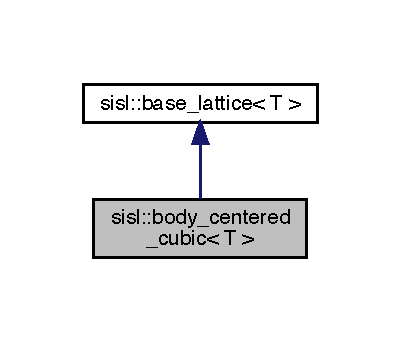
\includegraphics[width=192pt]{classsisl_1_1body__centered__cubic__inherit__graph}
\end{center}
\end{figure}


Collaboration diagram for sisl\+:\+:body\+\_\+centered\+\_\+cubic$<$ T $>$\+:\nopagebreak
\begin{figure}[H]
\begin{center}
\leavevmode
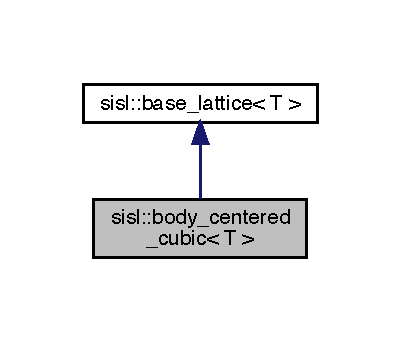
\includegraphics[width=192pt]{classsisl_1_1body__centered__cubic__coll__graph}
\end{center}
\end{figure}
\subsection*{Public Member Functions}
\begin{DoxyCompactItemize}
\item 
\mbox{\Hypertarget{classsisl_1_1body__centered__cubic_a061da4d24b45a2d4d2ebbc1577a05df9}\label{classsisl_1_1body__centered__cubic_a061da4d24b45a2d4d2ebbc1577a05df9}} 
\hyperlink{classsisl_1_1body__centered__cubic_a061da4d24b45a2d4d2ebbc1577a05df9}{body\+\_\+centered\+\_\+cubic} ()
\begin{DoxyCompactList}\small\item\em Dummy zero allocator for the CC lattice. \end{DoxyCompactList}\item 
\mbox{\Hypertarget{classsisl_1_1body__centered__cubic_a4d5c7c5f734201a1e235e7d0ede642a0}\label{classsisl_1_1body__centered__cubic_a4d5c7c5f734201a1e235e7d0ede642a0}} 
\hyperlink{classsisl_1_1body__centered__cubic_a4d5c7c5f734201a1e235e7d0ede642a0}{body\+\_\+centered\+\_\+cubic} (const int \&rx, const int \&ry, const int \&rz)
\begin{DoxyCompactList}\small\item\em Allocates a B\+CC lattice. This lattice includes all integer points in \mbox{[}0, rx\mbox{]} x \mbox{[}0, ry\mbox{]} x \mbox{[}0, rz\mbox{]}, with even Z parity note that this is inclusive. \end{DoxyCompactList}\item 
\mbox{\Hypertarget{classsisl_1_1body__centered__cubic_ac81d4da54d2487737a8066944b6b49dd}\label{classsisl_1_1body__centered__cubic_ac81d4da54d2487737a8066944b6b49dd}} 
\hyperlink{classsisl_1_1body__centered__cubic_ac81d4da54d2487737a8066944b6b49dd}{body\+\_\+centered\+\_\+cubic} (std\+::ifstream \&stream)
\begin{DoxyCompactList}\small\item\em Initializes a B\+CC lattice from a file stream. \end{DoxyCompactList}\item 
\mbox{\Hypertarget{classsisl_1_1body__centered__cubic_a413597e910db22f5aec4113ec6cbd36b}\label{classsisl_1_1body__centered__cubic_a413597e910db22f5aec4113ec6cbd36b}} 
virtual T \& \hyperlink{classsisl_1_1body__centered__cubic_a413597e910db22f5aec4113ec6cbd36b}{operator()} (int d0,...)
\begin{DoxyCompactList}\small\item\em Access a lattice site. Operators for accessing lattice sites. These index in the natural coordinate system of the lattice. \end{DoxyCompactList}\item 
\mbox{\Hypertarget{classsisl_1_1body__centered__cubic_af48bfe2b5475860672a421efc7fd0f41}\label{classsisl_1_1body__centered__cubic_af48bfe2b5475860672a421efc7fd0f41}} 
virtual const T \& \hyperlink{classsisl_1_1body__centered__cubic_af48bfe2b5475860672a421efc7fd0f41}{operator()} (int d0,...) const
\begin{DoxyCompactList}\small\item\em Access a lattice site. Operators for accessing lattice sites. These index in the natural coordinate system of the lattice. \end{DoxyCompactList}\item 
\mbox{\Hypertarget{classsisl_1_1body__centered__cubic_a2390a32744243127b2be774fd99871f3}\label{classsisl_1_1body__centered__cubic_a2390a32744243127b2be774fd99871f3}} 
virtual T \& \hyperlink{classsisl_1_1body__centered__cubic_a2390a32744243127b2be774fd99871f3}{operator()} (int $\ast$d)
\begin{DoxyCompactList}\small\item\em Access a lattice site. Operators for accessing lattice sites. These index in the natural coordinate system of the lattice. \end{DoxyCompactList}\item 
\mbox{\Hypertarget{classsisl_1_1body__centered__cubic_a7cbc3858d97fe98a25a0570323169aa4}\label{classsisl_1_1body__centered__cubic_a7cbc3858d97fe98a25a0570323169aa4}} 
virtual const T \& \hyperlink{classsisl_1_1body__centered__cubic_a7cbc3858d97fe98a25a0570323169aa4}{operator()} (int $\ast$d) const
\begin{DoxyCompactList}\small\item\em Access a lattice site. Operators for accessing lattice sites. These index in the natural coordinate system of the lattice. \end{DoxyCompactList}\item 
\mbox{\Hypertarget{classsisl_1_1body__centered__cubic_aa8aae2c66e2cf075a419bb8232fbd43b}\label{classsisl_1_1body__centered__cubic_aa8aae2c66e2cf075a419bb8232fbd43b}} 
virtual T \& \hyperlink{classsisl_1_1body__centered__cubic_aa8aae2c66e2cf075a419bb8232fbd43b}{operator()} (const \hyperlink{namespacesisl_acd18feee4026583db6185df2b25434aa}{lattice\+\_\+site} \&s)
\begin{DoxyCompactList}\small\item\em Access a lattice site. Operators for accessing lattice sites. These index in the natural coordinate system of the lattice. \end{DoxyCompactList}\item 
\mbox{\Hypertarget{classsisl_1_1body__centered__cubic_a279eb3385f2f252a30ad968951494922}\label{classsisl_1_1body__centered__cubic_a279eb3385f2f252a30ad968951494922}} 
virtual const T \& \hyperlink{classsisl_1_1body__centered__cubic_a279eb3385f2f252a30ad968951494922}{operator()} (const \hyperlink{namespacesisl_acd18feee4026583db6185df2b25434aa}{lattice\+\_\+site} \&s) const
\begin{DoxyCompactList}\small\item\em Access a lattice site. Operators for accessing lattice sites. These index in the natural coordinate system of the lattice. \end{DoxyCompactList}\item 
\mbox{\Hypertarget{classsisl_1_1body__centered__cubic_a6dfe90a15bb88786ac5c8b15cfe50285}\label{classsisl_1_1body__centered__cubic_a6dfe90a15bb88786ac5c8b15cfe50285}} 
virtual const unsigned int \hyperlink{classsisl_1_1body__centered__cubic_a6dfe90a15bb88786ac5c8b15cfe50285}{linear\+\_\+index} (int d0,...) const
\begin{DoxyCompactList}\small\item\em Uniquely index a lattice site This function return a linearized version of a lattice site, this allows one to uniquely associate a lattice site with an integer. \end{DoxyCompactList}\item 
\mbox{\Hypertarget{classsisl_1_1body__centered__cubic_a6f12217c00c0a417a80ef7c20b9281a8}\label{classsisl_1_1body__centered__cubic_a6f12217c00c0a417a80ef7c20b9281a8}} 
virtual const unsigned int \hyperlink{classsisl_1_1body__centered__cubic_a6f12217c00c0a417a80ef7c20b9281a8}{linear\+\_\+index} (int $\ast$d) const
\begin{DoxyCompactList}\small\item\em Uniquely index a lattice site This function return a linearized version of a lattice site, this allows one to uniquely associate a lattice site with an integer. \end{DoxyCompactList}\item 
\mbox{\Hypertarget{classsisl_1_1body__centered__cubic_aa34843f446ce5f8e3b0e64e78597d592}\label{classsisl_1_1body__centered__cubic_aa34843f446ce5f8e3b0e64e78597d592}} 
virtual const unsigned int \hyperlink{classsisl_1_1body__centered__cubic_aa34843f446ce5f8e3b0e64e78597d592}{linear\+\_\+index} (const \hyperlink{namespacesisl_acd18feee4026583db6185df2b25434aa}{lattice\+\_\+site} \&s) const
\begin{DoxyCompactList}\small\item\em Uniquely index a lattice site This function return a linearized version of a lattice site, this allows one to uniquely associate a lattice site with an integer. \end{DoxyCompactList}\item 
\mbox{\Hypertarget{classsisl_1_1body__centered__cubic_acff7112b5c40c548f1b693f087daeffb}\label{classsisl_1_1body__centered__cubic_acff7112b5c40c548f1b693f087daeffb}} 
virtual const \hyperlink{namespacesisl_a2069bd5374a9be042ff3ce3306d41e1a}{vector} \hyperlink{classsisl_1_1body__centered__cubic_acff7112b5c40c548f1b693f087daeffb}{get\+\_\+natural\+\_\+scales} () const
\begin{DoxyCompactList}\small\item\em Returns a natural scale so that the lattice sites would be scaled to within a unit hyper cube. \end{DoxyCompactList}\item 
\mbox{\Hypertarget{classsisl_1_1body__centered__cubic_a785d7bcf03ca3f6073d5d64c7dff8799}\label{classsisl_1_1body__centered__cubic_a785d7bcf03ca3f6073d5d64c7dff8799}} 
virtual const \hyperlink{namespacesisl_acd18feee4026583db6185df2b25434aa}{lattice\+\_\+site} \hyperlink{classsisl_1_1body__centered__cubic_a785d7bcf03ca3f6073d5d64c7dff8799}{get\+\_\+dimensions} () const
\begin{DoxyCompactList}\small\item\em Returns the integer extent of each dimension, that is, the lattice extends from \mbox{[}0, ret\mbox{[}i\mbox{]}\mbox{]} in each dimension. \end{DoxyCompactList}\item 
\mbox{\Hypertarget{classsisl_1_1body__centered__cubic_af853fa5d0bebb9e944a436777eb3570e}\label{classsisl_1_1body__centered__cubic_af853fa5d0bebb9e944a436777eb3570e}} 
virtual \hyperlink{namespacesisl_a2069bd5374a9be042ff3ce3306d41e1a}{vector} \hyperlink{classsisl_1_1body__centered__cubic_af853fa5d0bebb9e944a436777eb3570e}{get\+\_\+site\+\_\+position} (int d0,...) const
\begin{DoxyCompactList}\small\item\em Returns a value within the unit hyper cube that represents the given lattice site scaled within that unit hypercube. \end{DoxyCompactList}\item 
\mbox{\Hypertarget{classsisl_1_1body__centered__cubic_a7f9420a1a443beb5cdd23289ad91f4de}\label{classsisl_1_1body__centered__cubic_a7f9420a1a443beb5cdd23289ad91f4de}} 
virtual \hyperlink{namespacesisl_a2069bd5374a9be042ff3ce3306d41e1a}{vector} \hyperlink{classsisl_1_1body__centered__cubic_a7f9420a1a443beb5cdd23289ad91f4de}{get\+\_\+site\+\_\+position} (int $\ast$d) const
\begin{DoxyCompactList}\small\item\em Returns a value within the unit hyper cube that represents the given lattice site scaled withing that unit hypercube. \end{DoxyCompactList}\item 
\mbox{\Hypertarget{classsisl_1_1body__centered__cubic_a67cbe56fa247a8f787db629c59a2f3a9}\label{classsisl_1_1body__centered__cubic_a67cbe56fa247a8f787db629c59a2f3a9}} 
virtual \hyperlink{namespacesisl_a2069bd5374a9be042ff3ce3306d41e1a}{vector} \hyperlink{classsisl_1_1body__centered__cubic_a67cbe56fa247a8f787db629c59a2f3a9}{get\+\_\+site\+\_\+position} (const \hyperlink{namespacesisl_acd18feee4026583db6185df2b25434aa}{lattice\+\_\+site} \&s) const
\begin{DoxyCompactList}\small\item\em Returns a value within the unit hyper cube that represents the given lattice site scaled withing that unit hypercube. \end{DoxyCompactList}\item 
\mbox{\Hypertarget{classsisl_1_1body__centered__cubic_a4ee5d6c2c2ce3154aa62ca53a222510e}\label{classsisl_1_1body__centered__cubic_a4ee5d6c2c2ce3154aa62ca53a222510e}} 
virtual \hyperlink{namespacesisl_acd18feee4026583db6185df2b25434aa}{lattice\+\_\+site} \hyperlink{classsisl_1_1body__centered__cubic_a4ee5d6c2c2ce3154aa62ca53a222510e}{get\+\_\+nearest\+\_\+site} (const \hyperlink{namespacesisl_a2069bd5374a9be042ff3ce3306d41e1a}{vector} \&pt) const
\begin{DoxyCompactList}\small\item\em Returns the nearest lattice site for a given point within the unit hyper cube. \end{DoxyCompactList}\item 
\mbox{\Hypertarget{classsisl_1_1body__centered__cubic_a0cc4d7416cc84cf8914677131215b9ee}\label{classsisl_1_1body__centered__cubic_a0cc4d7416cc84cf8914677131215b9ee}} 
virtual bool \hyperlink{classsisl_1_1body__centered__cubic_a0cc4d7416cc84cf8914677131215b9ee}{is\+\_\+lattice\+\_\+site} (int d0,...) const
\begin{DoxyCompactList}\small\item\em Returns whether or not a lattice site truely corresponds to a valid lattice site on this particular lattice. \end{DoxyCompactList}\item 
\mbox{\Hypertarget{classsisl_1_1body__centered__cubic_a98d4d9250d92c3677c6b8d58e2f4d034}\label{classsisl_1_1body__centered__cubic_a98d4d9250d92c3677c6b8d58e2f4d034}} 
virtual bool \hyperlink{classsisl_1_1body__centered__cubic_a98d4d9250d92c3677c6b8d58e2f4d034}{is\+\_\+lattice\+\_\+site} (int $\ast$d) const
\begin{DoxyCompactList}\small\item\em Returns whether or not a lattice site truely corresponds to a valid lattice site on this particular lattice. \end{DoxyCompactList}\item 
\mbox{\Hypertarget{classsisl_1_1body__centered__cubic_a5347e1116144be97551c3baac90bc75d}\label{classsisl_1_1body__centered__cubic_a5347e1116144be97551c3baac90bc75d}} 
virtual bool \hyperlink{classsisl_1_1body__centered__cubic_a5347e1116144be97551c3baac90bc75d}{is\+\_\+lattice\+\_\+site} (const \hyperlink{namespacesisl_acd18feee4026583db6185df2b25434aa}{lattice\+\_\+site} \&s) const
\begin{DoxyCompactList}\small\item\em Returns whether or not a lattice\+\_\+site object truely corresponds to a valid lattice site on this particular lattice. \end{DoxyCompactList}\item 
\mbox{\Hypertarget{classsisl_1_1body__centered__cubic_ae892bd04e5b649a6aa48dc4f464d0f69}\label{classsisl_1_1body__centered__cubic_ae892bd04e5b649a6aa48dc4f464d0f69}} 
virtual bool \hyperlink{classsisl_1_1body__centered__cubic_ae892bd04e5b649a6aa48dc4f464d0f69}{is\+\_\+filled} (int d0,...) const
\begin{DoxyCompactList}\small\item\em Returns whether a lattice site actually contains a value. \end{DoxyCompactList}\item 
\mbox{\Hypertarget{classsisl_1_1body__centered__cubic_a8f40907ff91829e226bf224525b984b3}\label{classsisl_1_1body__centered__cubic_a8f40907ff91829e226bf224525b984b3}} 
virtual bool \hyperlink{classsisl_1_1body__centered__cubic_a8f40907ff91829e226bf224525b984b3}{is\+\_\+filled} (int $\ast$d) const
\begin{DoxyCompactList}\small\item\em Returns whether a lattice site actually contains a value. \end{DoxyCompactList}\item 
\mbox{\Hypertarget{classsisl_1_1body__centered__cubic_a1c60cd88d4ecd4d224cc198fa52dad44}\label{classsisl_1_1body__centered__cubic_a1c60cd88d4ecd4d224cc198fa52dad44}} 
virtual bool \hyperlink{classsisl_1_1body__centered__cubic_a1c60cd88d4ecd4d224cc198fa52dad44}{is\+\_\+filled} (const \hyperlink{namespacesisl_acd18feee4026583db6185df2b25434aa}{lattice\+\_\+site} \&s) const
\begin{DoxyCompactList}\small\item\em Returns whether a lattice site actually contains a value. \end{DoxyCompactList}\item 
\mbox{\Hypertarget{classsisl_1_1body__centered__cubic_ae46befbb818394f332b938d3b669581c}\label{classsisl_1_1body__centered__cubic_ae46befbb818394f332b938d3b669581c}} 
virtual void \hyperlink{classsisl_1_1body__centered__cubic_ae46befbb818394f332b938d3b669581c}{each\+\_\+site} (const std\+::function$<$ void(const \hyperlink{namespacesisl_acd18feee4026583db6185df2b25434aa}{lattice\+\_\+site} \&)$>$ \&func, bool parallel=false)
\begin{DoxyCompactList}\small\item\em Iterates over every lattice site contained within the dimensions of this lattice. \end{DoxyCompactList}\item 
\mbox{\Hypertarget{classsisl_1_1body__centered__cubic_a0adca596900e43f75eabf139c964d91f}\label{classsisl_1_1body__centered__cubic_a0adca596900e43f75eabf139c964d91f}} 
virtual std\+::string \hyperlink{classsisl_1_1body__centered__cubic_a0adca596900e43f75eabf139c964d91f}{get\+\_\+lattice\+\_\+name} () const
\begin{DoxyCompactList}\small\item\em Returns the name of this lattice. \end{DoxyCompactList}\item 
\mbox{\Hypertarget{classsisl_1_1body__centered__cubic_a6f80df144a39eba292b6430179ea8bc0}\label{classsisl_1_1body__centered__cubic_a6f80df144a39eba292b6430179ea8bc0}} 
virtual const int \hyperlink{classsisl_1_1body__centered__cubic_a6f80df144a39eba292b6430179ea8bc0}{number\+\_\+of\+\_\+lattice\+\_\+sites} () const
\begin{DoxyCompactList}\small\item\em Returns the theoretical number of sites within this lattice. \end{DoxyCompactList}\item 
\mbox{\Hypertarget{classsisl_1_1body__centered__cubic_adb35d1330a63d021eed98700f4cb0381}\label{classsisl_1_1body__centered__cubic_adb35d1330a63d021eed98700f4cb0381}} 
virtual bool \hyperlink{classsisl_1_1body__centered__cubic_adb35d1330a63d021eed98700f4cb0381}{dump\+\_\+to\+\_\+stream} (std\+::ofstream \&stream) const
\begin{DoxyCompactList}\small\item\em Dumps this lattice to a file stream. \end{DoxyCompactList}\item 
\mbox{\Hypertarget{classsisl_1_1body__centered__cubic_af017fb6d5b54b573bcfba03740e51160}\label{classsisl_1_1body__centered__cubic_af017fb6d5b54b573bcfba03740e51160}} 
virtual bool \hyperlink{classsisl_1_1body__centered__cubic_af017fb6d5b54b573bcfba03740e51160}{read\+\_\+from\+\_\+stream} (std\+::ifstream \&)
\begin{DoxyCompactList}\small\item\em Reads a lattice to a file stream, replacing all values. \end{DoxyCompactList}\item 
\mbox{\Hypertarget{classsisl_1_1body__centered__cubic_a705c45755b3b186e904a637aabc7026b}\label{classsisl_1_1body__centered__cubic_a705c45755b3b186e904a637aabc7026b}} 
virtual void \hyperlink{classsisl_1_1body__centered__cubic_a705c45755b3b186e904a637aabc7026b}{set\+\_\+extension\+\_\+type} (const \hyperlink{namespacesisl_aaf1f41d23ed37dacaa4c9f1bb6d3324f}{Lattice\+Extension\+Type} \&e, const \hyperlink{namespacesisl_af139f6f74488292ae48c0d71eaa5d4f1}{Lattice\+Region\+Shift} \&s)
\begin{DoxyCompactList}\small\item\em Sets how a lattice is extended for values that outside of the defined rectangular region. \end{DoxyCompactList}\end{DoxyCompactItemize}
\subsection*{Protected Member Functions}
\begin{DoxyCompactItemize}
\item 
\mbox{\Hypertarget{classsisl_1_1body__centered__cubic_a47fdb8d33daa6f699aad7ec63387fd93}\label{classsisl_1_1body__centered__cubic_a47fdb8d33daa6f699aad7ec63387fd93}} 
bool {\bfseries in\+\_\+bound} (const int \&i, const int \&j, const int \&k) const
\item 
\mbox{\Hypertarget{classsisl_1_1body__centered__cubic_a2b3b01a3855ca9509d6ff64518b2b5a0}\label{classsisl_1_1body__centered__cubic_a2b3b01a3855ca9509d6ff64518b2b5a0}} 
virtual const unsigned int {\bfseries linear\+\_\+index} (int d0, va\+\_\+list vl) const
\item 
\mbox{\Hypertarget{classsisl_1_1body__centered__cubic_a279eb7ccc6eeea3a16f960ffd2176b3c}\label{classsisl_1_1body__centered__cubic_a279eb7ccc6eeea3a16f960ffd2176b3c}} 
virtual T \& {\bfseries operator()} (int d0, va\+\_\+list vl)
\item 
\mbox{\Hypertarget{classsisl_1_1body__centered__cubic_ae3c39465ea275d0958d626fa4c044ede}\label{classsisl_1_1body__centered__cubic_ae3c39465ea275d0958d626fa4c044ede}} 
virtual const T \& {\bfseries operator()} (int d0, va\+\_\+list vl) const
\item 
\mbox{\Hypertarget{classsisl_1_1body__centered__cubic_ad4f59dcda9bc1e62272a9d2f01a1d164}\label{classsisl_1_1body__centered__cubic_ad4f59dcda9bc1e62272a9d2f01a1d164}} 
virtual bool {\bfseries is\+\_\+filled} (int d0, va\+\_\+list vl) const
\item 
\mbox{\Hypertarget{classsisl_1_1body__centered__cubic_ad370f360adfb1cfcf3d84387be565e29}\label{classsisl_1_1body__centered__cubic_ad370f360adfb1cfcf3d84387be565e29}} 
virtual bool {\bfseries is\+\_\+lattice\+\_\+site} (int d0, va\+\_\+list vl) const
\end{DoxyCompactItemize}


\subsection{Detailed Description}
\subsubsection*{template$<$class T$>$\newline
class sisl\+::body\+\_\+centered\+\_\+cubic$<$ T $>$}

Defines the body centered cubic lattice in 3d. 

The documentation for this class was generated from the following file\+:\begin{DoxyCompactItemize}
\item 
/\+Users/joshuahoracsek/\+Projects/sisl\+\_\+redux/include/sisl/lattice/3d/body\+\_\+centered\+\_\+cubic.\+hpp\end{DoxyCompactItemize}

\hypertarget{classsisl_1_1cartesian__cubic}{}\section{sisl\+:\+:cartesian\+\_\+cubic$<$ T $>$ Class Template Reference}
\label{classsisl_1_1cartesian__cubic}\index{sisl\+::cartesian\+\_\+cubic$<$ T $>$@{sisl\+::cartesian\+\_\+cubic$<$ T $>$}}


A specialized cubic Cartesian lattice class.  




{\ttfamily \#include $<$cartesian\+\_\+cubic.\+hpp$>$}



Inheritance diagram for sisl\+:\+:cartesian\+\_\+cubic$<$ T $>$\+:\nopagebreak
\begin{figure}[H]
\begin{center}
\leavevmode
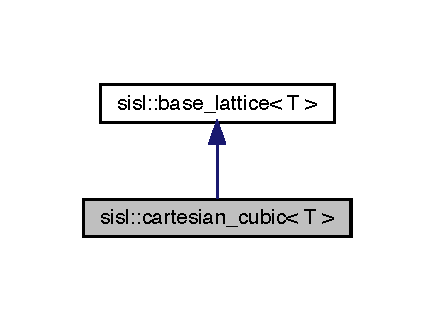
\includegraphics[width=208pt]{classsisl_1_1cartesian__cubic__inherit__graph}
\end{center}
\end{figure}


Collaboration diagram for sisl\+:\+:cartesian\+\_\+cubic$<$ T $>$\+:\nopagebreak
\begin{figure}[H]
\begin{center}
\leavevmode
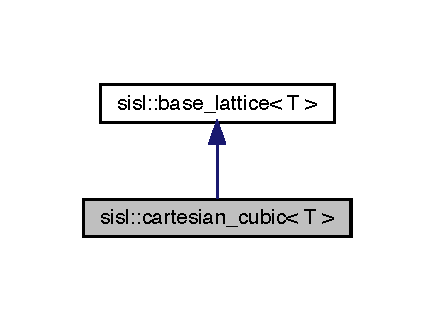
\includegraphics[width=208pt]{classsisl_1_1cartesian__cubic__coll__graph}
\end{center}
\end{figure}
\subsection*{Public Member Functions}
\begin{DoxyCompactItemize}
\item 
\mbox{\Hypertarget{classsisl_1_1cartesian__cubic_aa8c27fad87e2d7a21533b8649434fd2a}\label{classsisl_1_1cartesian__cubic_aa8c27fad87e2d7a21533b8649434fd2a}} 
\hyperlink{classsisl_1_1cartesian__cubic_aa8c27fad87e2d7a21533b8649434fd2a}{cartesian\+\_\+cubic} ()
\begin{DoxyCompactList}\small\item\em Dummy zero allocator for the CC lattice. \end{DoxyCompactList}\item 
\mbox{\Hypertarget{classsisl_1_1cartesian__cubic_a0dd7f488ca8c00be1eb1b51262534651}\label{classsisl_1_1cartesian__cubic_a0dd7f488ca8c00be1eb1b51262534651}} 
\hyperlink{classsisl_1_1cartesian__cubic_a0dd7f488ca8c00be1eb1b51262534651}{cartesian\+\_\+cubic} (unsigned int rx, unsigned int ry, unsigned int rz)
\begin{DoxyCompactList}\small\item\em Allocates a cubic cartesian lattice. This lattice includes all integer points in \mbox{[}0, rx\mbox{]} x \mbox{[}0, ry\mbox{]}, note that this is inclusive. \end{DoxyCompactList}\item 
\mbox{\Hypertarget{classsisl_1_1cartesian__cubic_a620b3d4bcd47b6e45e5ea01e41427bd5}\label{classsisl_1_1cartesian__cubic_a620b3d4bcd47b6e45e5ea01e41427bd5}} 
\hyperlink{classsisl_1_1cartesian__cubic_a620b3d4bcd47b6e45e5ea01e41427bd5}{cartesian\+\_\+cubic} (std\+::ifstream \&stream)
\begin{DoxyCompactList}\small\item\em Initializes a CC lattice from a file stream. \end{DoxyCompactList}\item 
\mbox{\Hypertarget{classsisl_1_1cartesian__cubic_acabf6e0c838717d24ef7dea204d2aa6f}\label{classsisl_1_1cartesian__cubic_acabf6e0c838717d24ef7dea204d2aa6f}} 
virtual T \& \hyperlink{classsisl_1_1cartesian__cubic_acabf6e0c838717d24ef7dea204d2aa6f}{operator()} (int d0,...)
\begin{DoxyCompactList}\small\item\em Access a lattice site. Operators for accessing lattice sites. These index in the natural coordinate system of the lattice. \end{DoxyCompactList}\item 
\mbox{\Hypertarget{classsisl_1_1cartesian__cubic_a8c3e5d7c1471efb3acf1ce5a946f0785}\label{classsisl_1_1cartesian__cubic_a8c3e5d7c1471efb3acf1ce5a946f0785}} 
virtual const T \& \hyperlink{classsisl_1_1cartesian__cubic_a8c3e5d7c1471efb3acf1ce5a946f0785}{operator()} (int d0,...) const
\begin{DoxyCompactList}\small\item\em Access a lattice site. Operators for accessing lattice sites. These index in the natural coordinate system of the lattice. \end{DoxyCompactList}\item 
\mbox{\Hypertarget{classsisl_1_1cartesian__cubic_a184aa9f24329d92c953a33d5d7df2f82}\label{classsisl_1_1cartesian__cubic_a184aa9f24329d92c953a33d5d7df2f82}} 
virtual T \& \hyperlink{classsisl_1_1cartesian__cubic_a184aa9f24329d92c953a33d5d7df2f82}{operator()} (int $\ast$d)
\begin{DoxyCompactList}\small\item\em Access a lattice site. Operators for accessing lattice sites. These index in the natural coordinate system of the lattice. \end{DoxyCompactList}\item 
\mbox{\Hypertarget{classsisl_1_1cartesian__cubic_a5ab2dfd1ffe49aea1e38384647b3c9b0}\label{classsisl_1_1cartesian__cubic_a5ab2dfd1ffe49aea1e38384647b3c9b0}} 
virtual const T \& \hyperlink{classsisl_1_1cartesian__cubic_a5ab2dfd1ffe49aea1e38384647b3c9b0}{operator()} (int $\ast$d) const
\begin{DoxyCompactList}\small\item\em Access a lattice site. Operators for accessing lattice sites. These index in the natural coordinate system of the lattice. \end{DoxyCompactList}\item 
\mbox{\Hypertarget{classsisl_1_1cartesian__cubic_a8cd465a0731e0d2e962329ba3a8e4f6e}\label{classsisl_1_1cartesian__cubic_a8cd465a0731e0d2e962329ba3a8e4f6e}} 
virtual T \& \hyperlink{classsisl_1_1cartesian__cubic_a8cd465a0731e0d2e962329ba3a8e4f6e}{operator()} (const \hyperlink{namespacesisl_acd18feee4026583db6185df2b25434aa}{lattice\+\_\+site} \&s)
\begin{DoxyCompactList}\small\item\em Access a lattice site. Operators for accessing lattice sites. These index in the natural coordinate system of the lattice. \end{DoxyCompactList}\item 
\mbox{\Hypertarget{classsisl_1_1cartesian__cubic_accef876590df812ec191ef66445fd6c7}\label{classsisl_1_1cartesian__cubic_accef876590df812ec191ef66445fd6c7}} 
virtual const T \& \hyperlink{classsisl_1_1cartesian__cubic_accef876590df812ec191ef66445fd6c7}{operator()} (const \hyperlink{namespacesisl_acd18feee4026583db6185df2b25434aa}{lattice\+\_\+site} \&s) const
\begin{DoxyCompactList}\small\item\em Access a lattice site. Operators for accessing lattice sites. These index in the natural coordinate system of the lattice. \end{DoxyCompactList}\item 
\mbox{\Hypertarget{classsisl_1_1cartesian__cubic_a50f99d5a3725d7f5cc019700bda8e44d}\label{classsisl_1_1cartesian__cubic_a50f99d5a3725d7f5cc019700bda8e44d}} 
virtual const unsigned int \hyperlink{classsisl_1_1cartesian__cubic_a50f99d5a3725d7f5cc019700bda8e44d}{linear\+\_\+index} (int d0,...) const
\begin{DoxyCompactList}\small\item\em Uniquely index a lattice site This function return a linearized version of a lattice site, this allows one to uniquely associate a lattice site with an integer. \end{DoxyCompactList}\item 
\mbox{\Hypertarget{classsisl_1_1cartesian__cubic_a42fc1105ab760fe34cb6863a79e7856b}\label{classsisl_1_1cartesian__cubic_a42fc1105ab760fe34cb6863a79e7856b}} 
virtual const unsigned int \hyperlink{classsisl_1_1cartesian__cubic_a42fc1105ab760fe34cb6863a79e7856b}{linear\+\_\+index} (int $\ast$d) const
\begin{DoxyCompactList}\small\item\em Uniquely index a lattice site This function return a linearized version of a lattice site, this allows one to uniquely associate a lattice site with an integer. \end{DoxyCompactList}\item 
\mbox{\Hypertarget{classsisl_1_1cartesian__cubic_a6029b29a29a5f6b056532c556ae883df}\label{classsisl_1_1cartesian__cubic_a6029b29a29a5f6b056532c556ae883df}} 
virtual const unsigned int \hyperlink{classsisl_1_1cartesian__cubic_a6029b29a29a5f6b056532c556ae883df}{linear\+\_\+index} (const \hyperlink{namespacesisl_acd18feee4026583db6185df2b25434aa}{lattice\+\_\+site} \&s) const
\begin{DoxyCompactList}\small\item\em Uniquely index a lattice site This function return a linearized version of a lattice site, this allows one to uniquely associate a lattice site with an integer. \end{DoxyCompactList}\item 
\mbox{\Hypertarget{classsisl_1_1cartesian__cubic_a52c6c0f97e7cb5dd2ead2c0a2a94e150}\label{classsisl_1_1cartesian__cubic_a52c6c0f97e7cb5dd2ead2c0a2a94e150}} 
virtual const \hyperlink{namespacesisl_a2069bd5374a9be042ff3ce3306d41e1a}{vector} \hyperlink{classsisl_1_1cartesian__cubic_a52c6c0f97e7cb5dd2ead2c0a2a94e150}{get\+\_\+natural\+\_\+scales} () const
\begin{DoxyCompactList}\small\item\em Returns a natural scale so that the lattice sites would be scaled to within a unit hyper cube. \end{DoxyCompactList}\item 
\mbox{\Hypertarget{classsisl_1_1cartesian__cubic_a4a578c3edf518c565288cfc2d15fcd67}\label{classsisl_1_1cartesian__cubic_a4a578c3edf518c565288cfc2d15fcd67}} 
virtual const \hyperlink{namespacesisl_acd18feee4026583db6185df2b25434aa}{lattice\+\_\+site} \hyperlink{classsisl_1_1cartesian__cubic_a4a578c3edf518c565288cfc2d15fcd67}{get\+\_\+dimensions} () const
\begin{DoxyCompactList}\small\item\em Returns the integer extent of each dimension, that is, the lattice extends from \mbox{[}0, ret\mbox{[}i\mbox{]}\mbox{]} in each dimension. \end{DoxyCompactList}\item 
\mbox{\Hypertarget{classsisl_1_1cartesian__cubic_ae4e02a25d580cad2e1475c14de4e1775}\label{classsisl_1_1cartesian__cubic_ae4e02a25d580cad2e1475c14de4e1775}} 
virtual \hyperlink{namespacesisl_a2069bd5374a9be042ff3ce3306d41e1a}{vector} \hyperlink{classsisl_1_1cartesian__cubic_ae4e02a25d580cad2e1475c14de4e1775}{get\+\_\+site\+\_\+position} (int d0,...) const
\begin{DoxyCompactList}\small\item\em Returns a value within the unit hyper cube that represents the given lattice site scaled withing that unit hypercube. \end{DoxyCompactList}\item 
\mbox{\Hypertarget{classsisl_1_1cartesian__cubic_a8737f47b33d8627a262ef6cd3682b259}\label{classsisl_1_1cartesian__cubic_a8737f47b33d8627a262ef6cd3682b259}} 
virtual \hyperlink{namespacesisl_a2069bd5374a9be042ff3ce3306d41e1a}{vector} \hyperlink{classsisl_1_1cartesian__cubic_a8737f47b33d8627a262ef6cd3682b259}{get\+\_\+site\+\_\+position} (int $\ast$d) const
\begin{DoxyCompactList}\small\item\em Returns a value within the unit hyper cube that represents the given lattice site scaled withing that unit hypercube. \end{DoxyCompactList}\item 
\mbox{\Hypertarget{classsisl_1_1cartesian__cubic_ad1f7419158bca45dfd6cc82d549e1149}\label{classsisl_1_1cartesian__cubic_ad1f7419158bca45dfd6cc82d549e1149}} 
virtual \hyperlink{namespacesisl_a2069bd5374a9be042ff3ce3306d41e1a}{vector} \hyperlink{classsisl_1_1cartesian__cubic_ad1f7419158bca45dfd6cc82d549e1149}{get\+\_\+site\+\_\+position} (const \hyperlink{namespacesisl_acd18feee4026583db6185df2b25434aa}{lattice\+\_\+site} \&s) const
\begin{DoxyCompactList}\small\item\em Returns a value within the unit hyper cube that represents the given lattice site scaled withing that unit hypercube. \end{DoxyCompactList}\item 
\mbox{\Hypertarget{classsisl_1_1cartesian__cubic_a75a8483c3ef02993c138d47236312954}\label{classsisl_1_1cartesian__cubic_a75a8483c3ef02993c138d47236312954}} 
virtual \hyperlink{namespacesisl_acd18feee4026583db6185df2b25434aa}{lattice\+\_\+site} \hyperlink{classsisl_1_1cartesian__cubic_a75a8483c3ef02993c138d47236312954}{get\+\_\+nearest\+\_\+site} (const \hyperlink{namespacesisl_a2069bd5374a9be042ff3ce3306d41e1a}{vector} \&pt) const
\begin{DoxyCompactList}\small\item\em Returns the nearest lattice site for a given point within the unit hyper cube. \end{DoxyCompactList}\item 
\mbox{\Hypertarget{classsisl_1_1cartesian__cubic_a24d53f68dc4a95343445a3edd7bc5d3d}\label{classsisl_1_1cartesian__cubic_a24d53f68dc4a95343445a3edd7bc5d3d}} 
virtual bool \hyperlink{classsisl_1_1cartesian__cubic_a24d53f68dc4a95343445a3edd7bc5d3d}{is\+\_\+lattice\+\_\+site} (int d0,...) const
\begin{DoxyCompactList}\small\item\em Returns whether or not a lattice site truely corresponds to a valid lattice site on this particular lattice. \end{DoxyCompactList}\item 
\mbox{\Hypertarget{classsisl_1_1cartesian__cubic_a3ae9596c32734a5b03eef4d7803d8ce4}\label{classsisl_1_1cartesian__cubic_a3ae9596c32734a5b03eef4d7803d8ce4}} 
virtual bool \hyperlink{classsisl_1_1cartesian__cubic_a3ae9596c32734a5b03eef4d7803d8ce4}{is\+\_\+lattice\+\_\+site} (int $\ast$d) const
\begin{DoxyCompactList}\small\item\em Returns whether or not a lattice site truely corresponds to a valid lattice site on this particular lattice. \end{DoxyCompactList}\item 
\mbox{\Hypertarget{classsisl_1_1cartesian__cubic_af82ea6f5e243e9a24ba95bb37b796546}\label{classsisl_1_1cartesian__cubic_af82ea6f5e243e9a24ba95bb37b796546}} 
virtual bool \hyperlink{classsisl_1_1cartesian__cubic_af82ea6f5e243e9a24ba95bb37b796546}{is\+\_\+lattice\+\_\+site} (const \hyperlink{namespacesisl_acd18feee4026583db6185df2b25434aa}{lattice\+\_\+site} \&) const
\begin{DoxyCompactList}\small\item\em Returns whether or not a lattice\+\_\+site object truely corresponds to a valid lattice site on this particular lattice. \end{DoxyCompactList}\item 
\mbox{\Hypertarget{classsisl_1_1cartesian__cubic_af1915dc2bc734e06d3cfff17d7da1a7f}\label{classsisl_1_1cartesian__cubic_af1915dc2bc734e06d3cfff17d7da1a7f}} 
virtual bool \hyperlink{classsisl_1_1cartesian__cubic_af1915dc2bc734e06d3cfff17d7da1a7f}{is\+\_\+filled} (int d0,...) const
\begin{DoxyCompactList}\small\item\em Returns whether a lattice site actually contains a value. \end{DoxyCompactList}\item 
\mbox{\Hypertarget{classsisl_1_1cartesian__cubic_a7fcd8a7cc29bc4857c384b9c9d5040d9}\label{classsisl_1_1cartesian__cubic_a7fcd8a7cc29bc4857c384b9c9d5040d9}} 
virtual bool \hyperlink{classsisl_1_1cartesian__cubic_a7fcd8a7cc29bc4857c384b9c9d5040d9}{is\+\_\+filled} (int $\ast$d) const
\begin{DoxyCompactList}\small\item\em Returns whether a lattice site actually contains a value. \end{DoxyCompactList}\item 
\mbox{\Hypertarget{classsisl_1_1cartesian__cubic_a68f4f410e2711d3cf1e4066679f1910d}\label{classsisl_1_1cartesian__cubic_a68f4f410e2711d3cf1e4066679f1910d}} 
virtual bool \hyperlink{classsisl_1_1cartesian__cubic_a68f4f410e2711d3cf1e4066679f1910d}{is\+\_\+filled} (const \hyperlink{namespacesisl_acd18feee4026583db6185df2b25434aa}{lattice\+\_\+site} \&s) const
\begin{DoxyCompactList}\small\item\em Returns whether a lattice site actually contains a value. \end{DoxyCompactList}\item 
\mbox{\Hypertarget{classsisl_1_1cartesian__cubic_a6e462e0f77044a855df84a3323660bff}\label{classsisl_1_1cartesian__cubic_a6e462e0f77044a855df84a3323660bff}} 
virtual void \hyperlink{classsisl_1_1cartesian__cubic_a6e462e0f77044a855df84a3323660bff}{each\+\_\+site} (const std\+::function$<$ void(const \hyperlink{namespacesisl_acd18feee4026583db6185df2b25434aa}{lattice\+\_\+site} \&)$>$ \&func, bool parallel=false)
\begin{DoxyCompactList}\small\item\em Iterates over every lattice site contained within the dimensions of this lattice. \end{DoxyCompactList}\item 
\mbox{\Hypertarget{classsisl_1_1cartesian__cubic_a9b076e76c2bffc4a0ed38d5fa7e65fad}\label{classsisl_1_1cartesian__cubic_a9b076e76c2bffc4a0ed38d5fa7e65fad}} 
virtual std\+::string \hyperlink{classsisl_1_1cartesian__cubic_a9b076e76c2bffc4a0ed38d5fa7e65fad}{get\+\_\+lattice\+\_\+name} () const
\begin{DoxyCompactList}\small\item\em Returns the name of this lattice. \end{DoxyCompactList}\item 
\mbox{\Hypertarget{classsisl_1_1cartesian__cubic_a1f6efaeaabe591bde7f9afa83a1f0699}\label{classsisl_1_1cartesian__cubic_a1f6efaeaabe591bde7f9afa83a1f0699}} 
virtual const int \hyperlink{classsisl_1_1cartesian__cubic_a1f6efaeaabe591bde7f9afa83a1f0699}{number\+\_\+of\+\_\+lattice\+\_\+sites} () const
\begin{DoxyCompactList}\small\item\em Returns the theoretical number of sites within this lattice. \end{DoxyCompactList}\item 
\mbox{\Hypertarget{classsisl_1_1cartesian__cubic_a00b578d2ad943a7181b591b5537a358d}\label{classsisl_1_1cartesian__cubic_a00b578d2ad943a7181b591b5537a358d}} 
virtual bool \hyperlink{classsisl_1_1cartesian__cubic_a00b578d2ad943a7181b591b5537a358d}{dump\+\_\+to\+\_\+stream} (std\+::ofstream \&stream) const
\begin{DoxyCompactList}\small\item\em Dumps this lattice to a file stream. \end{DoxyCompactList}\item 
\mbox{\Hypertarget{classsisl_1_1cartesian__cubic_ab3c5e58ee1b42f18d6bb86925088797d}\label{classsisl_1_1cartesian__cubic_ab3c5e58ee1b42f18d6bb86925088797d}} 
virtual bool \hyperlink{classsisl_1_1cartesian__cubic_ab3c5e58ee1b42f18d6bb86925088797d}{read\+\_\+from\+\_\+stream} (std\+::ifstream \&)
\begin{DoxyCompactList}\small\item\em Reads a lattice to a file stream, replacing all values. \end{DoxyCompactList}\item 
\mbox{\Hypertarget{classsisl_1_1cartesian__cubic_af25cab19b488abbfb22a86887c38ad06}\label{classsisl_1_1cartesian__cubic_af25cab19b488abbfb22a86887c38ad06}} 
virtual void \hyperlink{classsisl_1_1cartesian__cubic_af25cab19b488abbfb22a86887c38ad06}{set\+\_\+extension\+\_\+type} (const \hyperlink{namespacesisl_aaf1f41d23ed37dacaa4c9f1bb6d3324f}{Lattice\+Extension\+Type} \&e, const \hyperlink{namespacesisl_af139f6f74488292ae48c0d71eaa5d4f1}{Lattice\+Region\+Shift} \&s)
\begin{DoxyCompactList}\small\item\em Sets how a lattice is extended for values that outside of the defined rectangular region. \end{DoxyCompactList}\end{DoxyCompactItemize}
\subsection*{Protected Member Functions}
\begin{DoxyCompactItemize}
\item 
\mbox{\Hypertarget{classsisl_1_1cartesian__cubic_af5bf3656432d9da0559f50ed7607a562}\label{classsisl_1_1cartesian__cubic_af5bf3656432d9da0559f50ed7607a562}} 
virtual const unsigned int {\bfseries linear\+\_\+index} (int d0, va\+\_\+list vl) const
\item 
\mbox{\Hypertarget{classsisl_1_1cartesian__cubic_ab0035db1f1a2b045cbd99f060c158e3b}\label{classsisl_1_1cartesian__cubic_ab0035db1f1a2b045cbd99f060c158e3b}} 
virtual T \& {\bfseries operator()} (int d0, va\+\_\+list vl)
\item 
\mbox{\Hypertarget{classsisl_1_1cartesian__cubic_a176f010635742f3fe75f406759f731a5}\label{classsisl_1_1cartesian__cubic_a176f010635742f3fe75f406759f731a5}} 
virtual const T \& {\bfseries operator()} (int d0, va\+\_\+list vl) const
\item 
\mbox{\Hypertarget{classsisl_1_1cartesian__cubic_a882271145d3a8d2be007545a19ec7f99}\label{classsisl_1_1cartesian__cubic_a882271145d3a8d2be007545a19ec7f99}} 
virtual bool {\bfseries is\+\_\+filled} (int d0, va\+\_\+list vl) const
\item 
\mbox{\Hypertarget{classsisl_1_1cartesian__cubic_a803ae897f35a41e98f15dc5391f53943}\label{classsisl_1_1cartesian__cubic_a803ae897f35a41e98f15dc5391f53943}} 
virtual bool {\bfseries is\+\_\+lattice\+\_\+site} (int d0, va\+\_\+list vl) const
\end{DoxyCompactItemize}


\subsection{Detailed Description}
\subsubsection*{template$<$class T$>$\newline
class sisl\+::cartesian\+\_\+cubic$<$ T $>$}

A specialized cubic Cartesian lattice class. 

The documentation for this class was generated from the following file\+:\begin{DoxyCompactItemize}
\item 
/\+Users/joshuahoracsek/\+Projects/sisl\+\_\+redux/include/sisl/lattice/3d/cartesian\+\_\+cubic.\+hpp\end{DoxyCompactItemize}

\hypertarget{classsisl_1_1cartesian__planar}{}\section{sisl\+:\+:cartesian\+\_\+planar$<$ T $>$ Class Template Reference}
\label{classsisl_1_1cartesian__planar}\index{sisl\+::cartesian\+\_\+planar$<$ T $>$@{sisl\+::cartesian\+\_\+planar$<$ T $>$}}


A specialized Cartesian planar lattice class.  




{\ttfamily \#include $<$cartesian\+\_\+planar.\+hpp$>$}



Inheritance diagram for sisl\+:\+:cartesian\+\_\+planar$<$ T $>$\+:\nopagebreak
\begin{figure}[H]
\begin{center}
\leavevmode
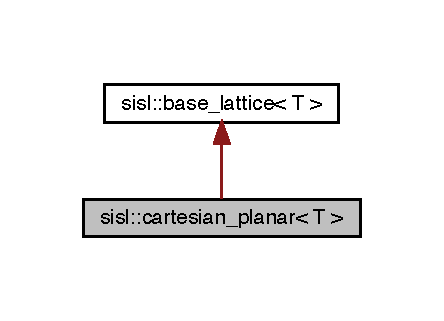
\includegraphics[width=213pt]{classsisl_1_1cartesian__planar__inherit__graph}
\end{center}
\end{figure}


Collaboration diagram for sisl\+:\+:cartesian\+\_\+planar$<$ T $>$\+:\nopagebreak
\begin{figure}[H]
\begin{center}
\leavevmode
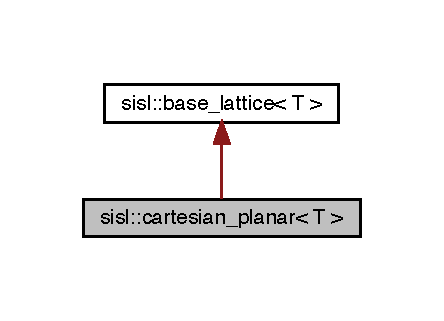
\includegraphics[width=213pt]{classsisl_1_1cartesian__planar__coll__graph}
\end{center}
\end{figure}
\subsection*{Public Member Functions}
\begin{DoxyCompactItemize}
\item 
\mbox{\Hypertarget{classsisl_1_1cartesian__planar_a4a18370588a67dac362c748d7bd46b04}\label{classsisl_1_1cartesian__planar_a4a18370588a67dac362c748d7bd46b04}} 
\hyperlink{classsisl_1_1cartesian__planar_a4a18370588a67dac362c748d7bd46b04}{cartesian\+\_\+planar} (unsigned int rx, unsigned int ry)
\begin{DoxyCompactList}\small\item\em Allocates a planar cartesian lattice. This lattice includes all integer points in \mbox{[}0, rx\mbox{]} x \mbox{[}0, ry\mbox{]}, note that this is inclusive. \end{DoxyCompactList}\item 
\mbox{\Hypertarget{classsisl_1_1cartesian__planar_a1e1a3b1c44748218d601edbdf1bed2d8}\label{classsisl_1_1cartesian__planar_a1e1a3b1c44748218d601edbdf1bed2d8}} 
virtual T \& \hyperlink{classsisl_1_1cartesian__planar_a1e1a3b1c44748218d601edbdf1bed2d8}{operator()} (int d0,...)
\begin{DoxyCompactList}\small\item\em Access a lattice site. Operators for accessing lattice sites. These index in the natural coordinate system of the lattice. \end{DoxyCompactList}\item 
\mbox{\Hypertarget{classsisl_1_1cartesian__planar_a92169a5cd0efd070fcadb9108b7fee0d}\label{classsisl_1_1cartesian__planar_a92169a5cd0efd070fcadb9108b7fee0d}} 
virtual const T \& \hyperlink{classsisl_1_1cartesian__planar_a92169a5cd0efd070fcadb9108b7fee0d}{operator()} (int d0,...) const
\begin{DoxyCompactList}\small\item\em Access a lattice site. Operators for accessing lattice sites. These index in the natural coordinate system of the lattice. \end{DoxyCompactList}\item 
\mbox{\Hypertarget{classsisl_1_1cartesian__planar_a20ef7e8f23c0e6bfd1bfea5816a0d424}\label{classsisl_1_1cartesian__planar_a20ef7e8f23c0e6bfd1bfea5816a0d424}} 
virtual T \& \hyperlink{classsisl_1_1cartesian__planar_a20ef7e8f23c0e6bfd1bfea5816a0d424}{operator()} (int $\ast$d)
\begin{DoxyCompactList}\small\item\em Access a lattice site. Operators for accessing lattice sites. These index in the natural coordinate system of the lattice. \end{DoxyCompactList}\item 
\mbox{\Hypertarget{classsisl_1_1cartesian__planar_a540abb67ec834261a6d41fd4b4db108f}\label{classsisl_1_1cartesian__planar_a540abb67ec834261a6d41fd4b4db108f}} 
virtual const T \& \hyperlink{classsisl_1_1cartesian__planar_a540abb67ec834261a6d41fd4b4db108f}{operator()} (int $\ast$d) const
\begin{DoxyCompactList}\small\item\em Access a lattice site. Operators for accessing lattice sites. These index in the natural coordinate system of the lattice. \end{DoxyCompactList}\item 
\mbox{\Hypertarget{classsisl_1_1cartesian__planar_a44af2be07514dec7db6509f1e7917f77}\label{classsisl_1_1cartesian__planar_a44af2be07514dec7db6509f1e7917f77}} 
virtual T \& \hyperlink{classsisl_1_1cartesian__planar_a44af2be07514dec7db6509f1e7917f77}{operator()} (const \hyperlink{namespacesisl_acd18feee4026583db6185df2b25434aa}{lattice\+\_\+site} \&s)
\begin{DoxyCompactList}\small\item\em Access a lattice site. Operators for accessing lattice sites. These index in the natural coordinate system of the lattice. \end{DoxyCompactList}\item 
\mbox{\Hypertarget{classsisl_1_1cartesian__planar_acfe8f3200b5b9414d08afeea20c4bafd}\label{classsisl_1_1cartesian__planar_acfe8f3200b5b9414d08afeea20c4bafd}} 
virtual const T \& \hyperlink{classsisl_1_1cartesian__planar_acfe8f3200b5b9414d08afeea20c4bafd}{operator()} (const \hyperlink{namespacesisl_acd18feee4026583db6185df2b25434aa}{lattice\+\_\+site} \&s) const
\begin{DoxyCompactList}\small\item\em Access a lattice site. Operators for accessing lattice sites. These index in the natural coordinate system of the lattice. \end{DoxyCompactList}\item 
\mbox{\Hypertarget{classsisl_1_1cartesian__planar_a3f30c34e162863d0ef83f3cde628f87f}\label{classsisl_1_1cartesian__planar_a3f30c34e162863d0ef83f3cde628f87f}} 
virtual const unsigned int \hyperlink{classsisl_1_1cartesian__planar_a3f30c34e162863d0ef83f3cde628f87f}{linear\+\_\+index} (int d0,...) const
\begin{DoxyCompactList}\small\item\em Uniquely index a lattice site This function return a linearized version of a lattice site, this allows one to uniquely associate a lattice site with an integer. \end{DoxyCompactList}\item 
\mbox{\Hypertarget{classsisl_1_1cartesian__planar_a4ef0287f2ed519a497615049c3e564bf}\label{classsisl_1_1cartesian__planar_a4ef0287f2ed519a497615049c3e564bf}} 
virtual const unsigned int \hyperlink{classsisl_1_1cartesian__planar_a4ef0287f2ed519a497615049c3e564bf}{linear\+\_\+index} (int $\ast$d) const
\begin{DoxyCompactList}\small\item\em Uniquely index a lattice site This function return a linearized version of a lattice site, this allows one to uniquely associate a lattice site with an integer. \end{DoxyCompactList}\item 
\mbox{\Hypertarget{classsisl_1_1cartesian__planar_ae96d9421f8640e2fee5d269e9ef40db1}\label{classsisl_1_1cartesian__planar_ae96d9421f8640e2fee5d269e9ef40db1}} 
virtual const unsigned int \hyperlink{classsisl_1_1cartesian__planar_ae96d9421f8640e2fee5d269e9ef40db1}{linear\+\_\+index} (const \hyperlink{namespacesisl_acd18feee4026583db6185df2b25434aa}{lattice\+\_\+site} \&s) const
\begin{DoxyCompactList}\small\item\em Uniquely index a lattice site This function return a linearized version of a lattice site, this allows one to uniquely associate a lattice site with an integer. \end{DoxyCompactList}\item 
\mbox{\Hypertarget{classsisl_1_1cartesian__planar_a352301fc39d8766ff2705879828b4dd4}\label{classsisl_1_1cartesian__planar_a352301fc39d8766ff2705879828b4dd4}} 
virtual const \hyperlink{namespacesisl_a2069bd5374a9be042ff3ce3306d41e1a}{vector} \hyperlink{classsisl_1_1cartesian__planar_a352301fc39d8766ff2705879828b4dd4}{get\+\_\+natural\+\_\+scales} () const
\begin{DoxyCompactList}\small\item\em Returns a natural scale so that the lattice sites would be scaled to within a unit hyper cube. \end{DoxyCompactList}\item 
\mbox{\Hypertarget{classsisl_1_1cartesian__planar_ab0dc277c7fc20bea7770c602d0157961}\label{classsisl_1_1cartesian__planar_ab0dc277c7fc20bea7770c602d0157961}} 
virtual const \hyperlink{namespacesisl_acd18feee4026583db6185df2b25434aa}{lattice\+\_\+site} \hyperlink{classsisl_1_1cartesian__planar_ab0dc277c7fc20bea7770c602d0157961}{get\+\_\+dimensions} () const
\begin{DoxyCompactList}\small\item\em Returns the integer extent of each dimension, that is, the lattice extends from \mbox{[}0, ret\mbox{[}i\mbox{]}\mbox{]} in each dimension. \end{DoxyCompactList}\item 
\mbox{\Hypertarget{classsisl_1_1cartesian__planar_a509fa024a5d4327f8b1ad81156605840}\label{classsisl_1_1cartesian__planar_a509fa024a5d4327f8b1ad81156605840}} 
virtual \hyperlink{namespacesisl_a2069bd5374a9be042ff3ce3306d41e1a}{vector} \hyperlink{classsisl_1_1cartesian__planar_a509fa024a5d4327f8b1ad81156605840}{get\+\_\+site\+\_\+position} (int d0,...) const
\begin{DoxyCompactList}\small\item\em Returns a value within the unit hyper cube that represents the given lattice site scaled withing that unit hypercube. \end{DoxyCompactList}\item 
\mbox{\Hypertarget{classsisl_1_1cartesian__planar_a75f123949a7c983bded8ad94024b739e}\label{classsisl_1_1cartesian__planar_a75f123949a7c983bded8ad94024b739e}} 
virtual \hyperlink{namespacesisl_a2069bd5374a9be042ff3ce3306d41e1a}{vector} \hyperlink{classsisl_1_1cartesian__planar_a75f123949a7c983bded8ad94024b739e}{get\+\_\+site\+\_\+position} (int $\ast$d) const
\begin{DoxyCompactList}\small\item\em Returns a value within the unit hyper cube that represents the given lattice site scaled withing that unit hypercube. \end{DoxyCompactList}\item 
\mbox{\Hypertarget{classsisl_1_1cartesian__planar_afd0200d6e7828295036af9f770f9bff4}\label{classsisl_1_1cartesian__planar_afd0200d6e7828295036af9f770f9bff4}} 
virtual \hyperlink{namespacesisl_a2069bd5374a9be042ff3ce3306d41e1a}{vector} \hyperlink{classsisl_1_1cartesian__planar_afd0200d6e7828295036af9f770f9bff4}{get\+\_\+site\+\_\+position} (const \hyperlink{namespacesisl_acd18feee4026583db6185df2b25434aa}{lattice\+\_\+site} \&s) const
\begin{DoxyCompactList}\small\item\em Returns a value within the unit hyper cube that represents the given lattice site scaled withing that unit hypercube. \end{DoxyCompactList}\item 
\mbox{\Hypertarget{classsisl_1_1cartesian__planar_a34e1464436af1ed48fad3c0a13251232}\label{classsisl_1_1cartesian__planar_a34e1464436af1ed48fad3c0a13251232}} 
virtual \hyperlink{namespacesisl_acd18feee4026583db6185df2b25434aa}{lattice\+\_\+site} \hyperlink{classsisl_1_1cartesian__planar_a34e1464436af1ed48fad3c0a13251232}{get\+\_\+nearest\+\_\+site} (const \hyperlink{namespacesisl_a2069bd5374a9be042ff3ce3306d41e1a}{vector} \&pt) const
\begin{DoxyCompactList}\small\item\em Returns the nearest lattice site for a given point within the unit hyper cube. \end{DoxyCompactList}\item 
\mbox{\Hypertarget{classsisl_1_1cartesian__planar_ac8ac23247a744622562aa511ff385f3a}\label{classsisl_1_1cartesian__planar_ac8ac23247a744622562aa511ff385f3a}} 
virtual bool \hyperlink{classsisl_1_1cartesian__planar_ac8ac23247a744622562aa511ff385f3a}{is\+\_\+lattice\+\_\+site} (int d0,...) const
\begin{DoxyCompactList}\small\item\em Returns whether or not a lattice site truely corresponds to a valid lattice site on this particular lattice. \end{DoxyCompactList}\item 
\mbox{\Hypertarget{classsisl_1_1cartesian__planar_abbd7c2c4b87293cf8eee569cf55ddb8a}\label{classsisl_1_1cartesian__planar_abbd7c2c4b87293cf8eee569cf55ddb8a}} 
virtual bool \hyperlink{classsisl_1_1cartesian__planar_abbd7c2c4b87293cf8eee569cf55ddb8a}{is\+\_\+lattice\+\_\+site} (int $\ast$d) const
\begin{DoxyCompactList}\small\item\em Returns whether or not a lattice site truely corresponds to a valid lattice site on this particular lattice. \end{DoxyCompactList}\item 
\mbox{\Hypertarget{classsisl_1_1cartesian__planar_a9ddeca1a05552b2a16cf7b02ca1beebd}\label{classsisl_1_1cartesian__planar_a9ddeca1a05552b2a16cf7b02ca1beebd}} 
virtual bool \hyperlink{classsisl_1_1cartesian__planar_a9ddeca1a05552b2a16cf7b02ca1beebd}{is\+\_\+lattice\+\_\+site} (const \hyperlink{namespacesisl_acd18feee4026583db6185df2b25434aa}{lattice\+\_\+site} \&) const
\begin{DoxyCompactList}\small\item\em Returns whether or not a lattice\+\_\+site object truely corresponds to a valid lattice site on this particular lattice. \end{DoxyCompactList}\item 
\mbox{\Hypertarget{classsisl_1_1cartesian__planar_a78b14af058713bf51eaff38e2109afee}\label{classsisl_1_1cartesian__planar_a78b14af058713bf51eaff38e2109afee}} 
virtual bool \hyperlink{classsisl_1_1cartesian__planar_a78b14af058713bf51eaff38e2109afee}{is\+\_\+filled} (int d0,...) const
\begin{DoxyCompactList}\small\item\em Returns whether a lattice site actually contains a value. \end{DoxyCompactList}\item 
\mbox{\Hypertarget{classsisl_1_1cartesian__planar_aa8066a6406ec8a5dc44121067c0cfb15}\label{classsisl_1_1cartesian__planar_aa8066a6406ec8a5dc44121067c0cfb15}} 
virtual bool \hyperlink{classsisl_1_1cartesian__planar_aa8066a6406ec8a5dc44121067c0cfb15}{is\+\_\+filled} (int $\ast$d) const
\begin{DoxyCompactList}\small\item\em Returns whether a lattice site actually contains a value. \end{DoxyCompactList}\item 
\mbox{\Hypertarget{classsisl_1_1cartesian__planar_a5dd470e0b4d0966c38946c7e384d4090}\label{classsisl_1_1cartesian__planar_a5dd470e0b4d0966c38946c7e384d4090}} 
virtual bool \hyperlink{classsisl_1_1cartesian__planar_a5dd470e0b4d0966c38946c7e384d4090}{is\+\_\+filled} (const \hyperlink{namespacesisl_acd18feee4026583db6185df2b25434aa}{lattice\+\_\+site} \&s) const
\begin{DoxyCompactList}\small\item\em Returns whether a lattice site actually contains a value. \end{DoxyCompactList}\item 
\mbox{\Hypertarget{classsisl_1_1cartesian__planar_a8b1edfccbcc7bfbd9bd596d822fe51ea}\label{classsisl_1_1cartesian__planar_a8b1edfccbcc7bfbd9bd596d822fe51ea}} 
virtual void \hyperlink{classsisl_1_1cartesian__planar_a8b1edfccbcc7bfbd9bd596d822fe51ea}{each\+\_\+site} (const std\+::function$<$ void(const \hyperlink{namespacesisl_acd18feee4026583db6185df2b25434aa}{lattice\+\_\+site} \&)$>$ \&func, bool parallel=false)
\begin{DoxyCompactList}\small\item\em Iterates over every lattice site contained within the dimensions of this lattice. \end{DoxyCompactList}\item 
\mbox{\Hypertarget{classsisl_1_1cartesian__planar_ac71927dde6e99d60d8e5fe57601ca5a7}\label{classsisl_1_1cartesian__planar_ac71927dde6e99d60d8e5fe57601ca5a7}} 
virtual std\+::string \hyperlink{classsisl_1_1cartesian__planar_ac71927dde6e99d60d8e5fe57601ca5a7}{get\+\_\+lattice\+\_\+name} () const
\begin{DoxyCompactList}\small\item\em Returns the name of this lattice. \end{DoxyCompactList}\item 
\mbox{\Hypertarget{classsisl_1_1cartesian__planar_a1c56e22aac7799696512deecef69fc2b}\label{classsisl_1_1cartesian__planar_a1c56e22aac7799696512deecef69fc2b}} 
virtual const int \hyperlink{classsisl_1_1cartesian__planar_a1c56e22aac7799696512deecef69fc2b}{number\+\_\+of\+\_\+lattice\+\_\+sites} () const
\begin{DoxyCompactList}\small\item\em Returns the theoretical number of sites within this lattice. \end{DoxyCompactList}\item 
\mbox{\Hypertarget{classsisl_1_1cartesian__planar_a7870c4bc416767b53ef92812ef628523}\label{classsisl_1_1cartesian__planar_a7870c4bc416767b53ef92812ef628523}} 
virtual bool \hyperlink{classsisl_1_1cartesian__planar_a7870c4bc416767b53ef92812ef628523}{dump\+\_\+to\+\_\+stream} (std\+::ofstream \&) const
\begin{DoxyCompactList}\small\item\em Dumps this lattice to a file stream. \end{DoxyCompactList}\item 
\mbox{\Hypertarget{classsisl_1_1cartesian__planar_a683dc519e155eac540f1ef2bdd4f36fd}\label{classsisl_1_1cartesian__planar_a683dc519e155eac540f1ef2bdd4f36fd}} 
virtual bool \hyperlink{classsisl_1_1cartesian__planar_a683dc519e155eac540f1ef2bdd4f36fd}{read\+\_\+from\+\_\+stream} (std\+::ifstream \&)
\begin{DoxyCompactList}\small\item\em Reads a lattice to a file stream, replacing all values. \end{DoxyCompactList}\item 
\mbox{\Hypertarget{classsisl_1_1cartesian__planar_af8a148504e8c32b2582edfacd22247ed}\label{classsisl_1_1cartesian__planar_af8a148504e8c32b2582edfacd22247ed}} 
virtual void \hyperlink{classsisl_1_1cartesian__planar_af8a148504e8c32b2582edfacd22247ed}{set\+\_\+extension\+\_\+type} (const \hyperlink{namespacesisl_aaf1f41d23ed37dacaa4c9f1bb6d3324f}{Lattice\+Extension\+Type} \&e, const \hyperlink{namespacesisl_af139f6f74488292ae48c0d71eaa5d4f1}{Lattice\+Region\+Shift} \&s)
\begin{DoxyCompactList}\small\item\em Sets how a lattice is extended for values that outside of the defined rectangular region. \end{DoxyCompactList}\end{DoxyCompactItemize}
\subsection*{Protected Member Functions}
\begin{DoxyCompactItemize}
\item 
\mbox{\Hypertarget{classsisl_1_1cartesian__planar_a2091fb860fcb63177a2c8916a39c6bf9}\label{classsisl_1_1cartesian__planar_a2091fb860fcb63177a2c8916a39c6bf9}} 
virtual const unsigned int {\bfseries linear\+\_\+index} (int d0, va\+\_\+list vl) const
\item 
\mbox{\Hypertarget{classsisl_1_1cartesian__planar_aa257a635acd3a8dc75366147068b05af}\label{classsisl_1_1cartesian__planar_aa257a635acd3a8dc75366147068b05af}} 
virtual T \& {\bfseries operator()} (int d0, va\+\_\+list vl)
\item 
\mbox{\Hypertarget{classsisl_1_1cartesian__planar_a935f45a08742e35d1e159eb35e014f58}\label{classsisl_1_1cartesian__planar_a935f45a08742e35d1e159eb35e014f58}} 
virtual const T \& {\bfseries operator()} (int d0, va\+\_\+list vl) const
\item 
\mbox{\Hypertarget{classsisl_1_1cartesian__planar_a4ee4fd317136a64eac6353a7bfc8a2cd}\label{classsisl_1_1cartesian__planar_a4ee4fd317136a64eac6353a7bfc8a2cd}} 
virtual bool {\bfseries is\+\_\+filled} (int d0, va\+\_\+list vl) const
\item 
\mbox{\Hypertarget{classsisl_1_1cartesian__planar_a0f48cf84a1070fc116468c7631207fdd}\label{classsisl_1_1cartesian__planar_a0f48cf84a1070fc116468c7631207fdd}} 
virtual bool {\bfseries is\+\_\+lattice\+\_\+site} (int d0, va\+\_\+list vl) const
\end{DoxyCompactItemize}


\subsection{Detailed Description}
\subsubsection*{template$<$class T$>$\newline
class sisl\+::cartesian\+\_\+planar$<$ T $>$}

A specialized Cartesian planar lattice class. 

The documentation for this class was generated from the following file\+:\begin{DoxyCompactItemize}
\item 
/\+Users/joshuahoracsek/\+Projects/sisl\+\_\+redux/include/sisl/lattice/2d/cartesian\+\_\+planar.\+hpp\end{DoxyCompactItemize}

\hypertarget{classsisl_1_1function}{}\section{sisl\+:\+:function Class Reference}
\label{classsisl_1_1function}\index{sisl\+::function@{sisl\+::function}}


Abstract base class for a function. Defines a function that is valid over all R$^\wedge$n, it\textquotesingle{}s up to the underlying implementation to decide how those values map to real values.  




{\ttfamily \#include $<$base\+\_\+function.\+hpp$>$}



Inheritance diagram for sisl\+:\+:function\+:\nopagebreak
\begin{figure}[H]
\begin{center}
\leavevmode
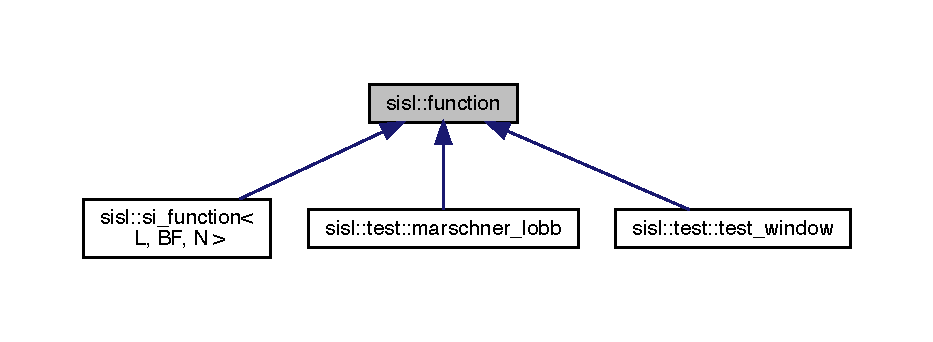
\includegraphics[width=350pt]{classsisl_1_1function__inherit__graph}
\end{center}
\end{figure}
\subsection*{Public Member Functions}
\begin{DoxyCompactItemize}
\item 
\mbox{\Hypertarget{classsisl_1_1function_afeac9ff55daf5e514e07ce93e2159c67}\label{classsisl_1_1function_afeac9ff55daf5e514e07ce93e2159c67}} 
virtual const double \hyperlink{classsisl_1_1function_afeac9ff55daf5e514e07ce93e2159c67}{operator()} (double d0,...) const =0
\begin{DoxyCompactList}\small\item\em Evaluate the function at a point. Evaluate the function at a point. \end{DoxyCompactList}\item 
\mbox{\Hypertarget{classsisl_1_1function_ab7cd4c0f5cc11e5c45a087338faf659f}\label{classsisl_1_1function_ab7cd4c0f5cc11e5c45a087338faf659f}} 
virtual const double \hyperlink{classsisl_1_1function_ab7cd4c0f5cc11e5c45a087338faf659f}{operator()} (const \hyperlink{namespacesisl_a2069bd5374a9be042ff3ce3306d41e1a}{vector} \&p) const =0
\begin{DoxyCompactList}\small\item\em Evaluate the function at a point. \end{DoxyCompactList}\item 
\mbox{\Hypertarget{classsisl_1_1function_a895e783c03f56af75f0b722822b20d4b}\label{classsisl_1_1function_a895e783c03f56af75f0b722822b20d4b}} 
virtual const double \hyperlink{classsisl_1_1function_a895e783c03f56af75f0b722822b20d4b}{eval} (double d0,...)
\begin{DoxyCompactList}\small\item\em Evaluate the function at a point. \end{DoxyCompactList}\item 
\mbox{\Hypertarget{classsisl_1_1function_ae2644d84c32f0b9e8a167735e26bca88}\label{classsisl_1_1function_ae2644d84c32f0b9e8a167735e26bca88}} 
virtual const double \hyperlink{classsisl_1_1function_ae2644d84c32f0b9e8a167735e26bca88}{eval} (const \hyperlink{namespacesisl_a2069bd5374a9be042ff3ce3306d41e1a}{vector} \&p)
\begin{DoxyCompactList}\small\item\em Evaluate the function at a point. \end{DoxyCompactList}\item 
\mbox{\Hypertarget{classsisl_1_1function_a520bfaebbd09c1d8678a129c548d4b1a}\label{classsisl_1_1function_a520bfaebbd09c1d8678a129c548d4b1a}} 
virtual const double \hyperlink{classsisl_1_1function_a520bfaebbd09c1d8678a129c548d4b1a}{d} (int component, double d0,...) const =0
\begin{DoxyCompactList}\small\item\em Evaluate the derivative of a function at a point. \end{DoxyCompactList}\item 
\mbox{\Hypertarget{classsisl_1_1function_a43aca1cd5bfa726e687c6cbe16d2c0e3}\label{classsisl_1_1function_a43aca1cd5bfa726e687c6cbe16d2c0e3}} 
virtual const double \hyperlink{classsisl_1_1function_a43aca1cd5bfa726e687c6cbe16d2c0e3}{d} (int component, const \hyperlink{namespacesisl_a2069bd5374a9be042ff3ce3306d41e1a}{vector} \&p) const =0
\begin{DoxyCompactList}\small\item\em Evaluate the derivative of a function at a point. \end{DoxyCompactList}\item 
\mbox{\Hypertarget{classsisl_1_1function_a7db0b15b30f7a7fedf6a3bed021ca56a}\label{classsisl_1_1function_a7db0b15b30f7a7fedf6a3bed021ca56a}} 
virtual const \hyperlink{namespacesisl_a2069bd5374a9be042ff3ce3306d41e1a}{vector} \hyperlink{classsisl_1_1function_a7db0b15b30f7a7fedf6a3bed021ca56a}{grad} (double d0,...) const =0
\begin{DoxyCompactList}\small\item\em Evaluate the gradient of the function at a point. \end{DoxyCompactList}\item 
\mbox{\Hypertarget{classsisl_1_1function_ad967b1e86a0b7ebaf9f1da9508052adf}\label{classsisl_1_1function_ad967b1e86a0b7ebaf9f1da9508052adf}} 
virtual const \hyperlink{namespacesisl_a2069bd5374a9be042ff3ce3306d41e1a}{vector} \hyperlink{classsisl_1_1function_ad967b1e86a0b7ebaf9f1da9508052adf}{grad} (const \hyperlink{namespacesisl_a2069bd5374a9be042ff3ce3306d41e1a}{vector} \&p) const =0
\begin{DoxyCompactList}\small\item\em Evaluate the gradient of the function at a point. \end{DoxyCompactList}\item 
\mbox{\Hypertarget{classsisl_1_1function_ab4cdf43f4187c937813f8184e347a9c9}\label{classsisl_1_1function_ab4cdf43f4187c937813f8184e347a9c9}} 
virtual const double \hyperlink{classsisl_1_1function_ab4cdf43f4187c937813f8184e347a9c9}{n\+\_\+d} (const \hyperlink{namespacesisl_adc492e1c166a136d08b283394d81cd71}{int\+\_\+tuple} \&order, double d0,...) const =0
\begin{DoxyCompactList}\small\item\em Evaluate the n\textquotesingle{}th partial derivative at a point. \end{DoxyCompactList}\item 
\mbox{\Hypertarget{classsisl_1_1function_ae7609877344e1b150638bfdc1f312a6e}\label{classsisl_1_1function_ae7609877344e1b150638bfdc1f312a6e}} 
virtual const double \hyperlink{classsisl_1_1function_ae7609877344e1b150638bfdc1f312a6e}{n\+\_\+d} (const \hyperlink{namespacesisl_adc492e1c166a136d08b283394d81cd71}{int\+\_\+tuple} \&order, \hyperlink{namespacesisl_a2069bd5374a9be042ff3ce3306d41e1a}{vector} \&p) const =0
\begin{DoxyCompactList}\small\item\em Evaluate the n\textquotesingle{}th partial derivative at a point. \end{DoxyCompactList}\item 
\mbox{\Hypertarget{classsisl_1_1function_abad7dc378805d859b1afa020565828be}\label{classsisl_1_1function_abad7dc378805d859b1afa020565828be}} 
virtual const int \hyperlink{classsisl_1_1function_abad7dc378805d859b1afa020565828be}{dim} () const =0
\begin{DoxyCompactList}\small\item\em Returns the input dimension of this function. \end{DoxyCompactList}\end{DoxyCompactItemize}


\subsection{Detailed Description}
Abstract base class for a function. Defines a function that is valid over all R$^\wedge$n, it\textquotesingle{}s up to the underlying implementation to decide how those values map to real values. 

The documentation for this class was generated from the following file\+:\begin{DoxyCompactItemize}
\item 
/\+Users/joshuahoracsek/\+Projects/sisl\+\_\+redux/include/sisl/function/base\+\_\+function.\+hpp\end{DoxyCompactItemize}

\hypertarget{classsisl_1_1utility_1_1isosurface}{}\section{sisl\+:\+:utility\+:\+:isosurface Class Reference}
\label{classsisl_1_1utility_1_1isosurface}\index{sisl\+::utility\+::isosurface@{sisl\+::utility\+::isosurface}}


An implementation of marching cubes.  




{\ttfamily \#include $<$iso\+\_\+surface.\+hpp$>$}

\subsection*{Public Member Functions}
\begin{DoxyCompactItemize}
\item 
void \hyperlink{classsisl_1_1utility_1_1isosurface_a27be7f0e3449d03e955df77e5944d5db}{set\+\_\+shading\+\_\+stepsize} (const double \&ss)
\begin{DoxyCompactList}\small\item\em Set heuristic parameters. \end{DoxyCompactList}\item 
void \hyperlink{classsisl_1_1utility_1_1isosurface_ad81b29590b262cf30286591090eabb13}{march\+\_\+function} (\hyperlink{classsisl_1_1function}{function} $\ast$f, const double \&iso\+Value, const double \&step\+Size, \hyperlink{namespacesisl_a2069bd5374a9be042ff3ce3306d41e1a}{sisl\+::vector} origin, \hyperlink{namespacesisl_a2069bd5374a9be042ff3ce3306d41e1a}{sisl\+::vector} extent, bool flip\+\_\+normal=false, \hyperlink{classsisl_1_1function}{sisl\+::function} $\ast$dx=nullptr, \hyperlink{classsisl_1_1function}{sisl\+::function} $\ast$dy=nullptr, \hyperlink{classsisl_1_1function}{sisl\+::function} $\ast$dz=nullptr)
\begin{DoxyCompactList}\small\item\em March isosurface. \end{DoxyCompactList}\item 
bool \hyperlink{classsisl_1_1utility_1_1isosurface_ada6c1709527aaee83f1d6e616172b1d4}{write\+\_\+surface} (const std\+::string \&out) const
\begin{DoxyCompactList}\small\item\em Output file. \end{DoxyCompactList}\item 
void \hyperlink{classsisl_1_1utility_1_1isosurface_a73bd6c29b9a5a1ff6f34120d2dac5d65}{apply\+\_\+transform} (const \hyperlink{namespacesisl_a2ef12d285ca3e626c05abbdec1f8a679}{transform} \&Tr)
\begin{DoxyCompactList}\small\item\em Transform mesh. \end{DoxyCompactList}\end{DoxyCompactItemize}


\subsection{Detailed Description}
An implementation of marching cubes. 

\subsection{Member Function Documentation}
\mbox{\Hypertarget{classsisl_1_1utility_1_1isosurface_a73bd6c29b9a5a1ff6f34120d2dac5d65}\label{classsisl_1_1utility_1_1isosurface_a73bd6c29b9a5a1ff6f34120d2dac5d65}} 
\index{sisl\+::utility\+::isosurface@{sisl\+::utility\+::isosurface}!apply\+\_\+transform@{apply\+\_\+transform}}
\index{apply\+\_\+transform@{apply\+\_\+transform}!sisl\+::utility\+::isosurface@{sisl\+::utility\+::isosurface}}
\subsubsection{\texorpdfstring{apply\+\_\+transform()}{apply\_transform()}}
{\footnotesize\ttfamily void sisl\+::utility\+::isosurface\+::apply\+\_\+transform (\begin{DoxyParamCaption}\item[{const \hyperlink{namespacesisl_a2ef12d285ca3e626c05abbdec1f8a679}{transform} \&}]{Tr }\end{DoxyParamCaption})\hspace{0.3cm}{\ttfamily [inline]}}



Transform mesh. 

Applies a transformation matrix to the vertices of the levelset. 
\begin{DoxyParams}{Parameters}
{\em Tr} & a transformation matrix. \\
\hline
\end{DoxyParams}
\mbox{\Hypertarget{classsisl_1_1utility_1_1isosurface_ad81b29590b262cf30286591090eabb13}\label{classsisl_1_1utility_1_1isosurface_ad81b29590b262cf30286591090eabb13}} 
\index{sisl\+::utility\+::isosurface@{sisl\+::utility\+::isosurface}!march\+\_\+function@{march\+\_\+function}}
\index{march\+\_\+function@{march\+\_\+function}!sisl\+::utility\+::isosurface@{sisl\+::utility\+::isosurface}}
\subsubsection{\texorpdfstring{march\+\_\+function()}{march\_function()}}
{\footnotesize\ttfamily void sisl\+::utility\+::isosurface\+::march\+\_\+function (\begin{DoxyParamCaption}\item[{\hyperlink{classsisl_1_1function}{function} $\ast$}]{f,  }\item[{const double \&}]{iso\+Value,  }\item[{const double \&}]{step\+Size,  }\item[{\hyperlink{namespacesisl_a2069bd5374a9be042ff3ce3306d41e1a}{sisl\+::vector}}]{origin,  }\item[{\hyperlink{namespacesisl_a2069bd5374a9be042ff3ce3306d41e1a}{sisl\+::vector}}]{extent,  }\item[{bool}]{flip\+\_\+normal = {\ttfamily false},  }\item[{\hyperlink{classsisl_1_1function}{sisl\+::function} $\ast$}]{dx = {\ttfamily nullptr},  }\item[{\hyperlink{classsisl_1_1function}{sisl\+::function} $\ast$}]{dy = {\ttfamily nullptr},  }\item[{\hyperlink{classsisl_1_1function}{sisl\+::function} $\ast$}]{dz = {\ttfamily nullptr} }\end{DoxyParamCaption})\hspace{0.3cm}{\ttfamily [inline]}}



March isosurface. 

Runs marching cubes (with corrected ambiguities) over f. It starts at origin, and marches a prismic volume with the dimensions in extent. If the dx,dy,dz are provided, then they will be used as the normal for the mesh, if not, then this function will attempt to use the grad member of the f. If that doesn\textquotesingle{}t work, it\textquotesingle{}ll use a divided difference to approximate the shading. The step size for this can be set via set\+\_\+shading\+\_\+stepsize.


\begin{DoxyParams}{Parameters}
{\em f} & the input function \\
\hline
{\em iso\+Value} & The iso value to extract \\
\hline
{\em step\+Size} & The size of steps, or the length of the edges of the cubes \\
\hline
{\em origin} & Where the marching begins in space \\
\hline
{\em extent} & The dimensions of the volume to march over \\
\hline
{\em flip\+\_\+normal} & Whether to flip the output normal. \\
\hline
{\em dx,dy,dz} & If specified, these are functions to use for the dx dy and dz gradient components. \\
\hline
\end{DoxyParams}
\mbox{\Hypertarget{classsisl_1_1utility_1_1isosurface_a27be7f0e3449d03e955df77e5944d5db}\label{classsisl_1_1utility_1_1isosurface_a27be7f0e3449d03e955df77e5944d5db}} 
\index{sisl\+::utility\+::isosurface@{sisl\+::utility\+::isosurface}!set\+\_\+shading\+\_\+stepsize@{set\+\_\+shading\+\_\+stepsize}}
\index{set\+\_\+shading\+\_\+stepsize@{set\+\_\+shading\+\_\+stepsize}!sisl\+::utility\+::isosurface@{sisl\+::utility\+::isosurface}}
\subsubsection{\texorpdfstring{set\+\_\+shading\+\_\+stepsize()}{set\_shading\_stepsize()}}
{\footnotesize\ttfamily void sisl\+::utility\+::isosurface\+::set\+\_\+shading\+\_\+stepsize (\begin{DoxyParamCaption}\item[{const double \&}]{ss }\end{DoxyParamCaption})\hspace{0.3cm}{\ttfamily [inline]}}



Set heuristic parameters. 

If the function we\textquotesingle{}re marching has to rely on using a heuristic for shading, then we\textquotesingle{}ll use ss to do a finite difference to calculate the partial derivatives in x y z.


\begin{DoxyParams}{Parameters}
{\em ss} & Step size for gradient computation \\
\hline
\end{DoxyParams}
\mbox{\Hypertarget{classsisl_1_1utility_1_1isosurface_ada6c1709527aaee83f1d6e616172b1d4}\label{classsisl_1_1utility_1_1isosurface_ada6c1709527aaee83f1d6e616172b1d4}} 
\index{sisl\+::utility\+::isosurface@{sisl\+::utility\+::isosurface}!write\+\_\+surface@{write\+\_\+surface}}
\index{write\+\_\+surface@{write\+\_\+surface}!sisl\+::utility\+::isosurface@{sisl\+::utility\+::isosurface}}
\subsubsection{\texorpdfstring{write\+\_\+surface()}{write\_surface()}}
{\footnotesize\ttfamily bool sisl\+::utility\+::isosurface\+::write\+\_\+surface (\begin{DoxyParamCaption}\item[{const std\+::string \&}]{out }\end{DoxyParamCaption}) const\hspace{0.3cm}{\ttfamily [inline]}}



Output file. 

Writes the marched isosurface into a file. 
\begin{DoxyParams}{Parameters}
{\em out} & the filename to output the ply to. \\
\hline
\end{DoxyParams}


The documentation for this class was generated from the following file\+:\begin{DoxyCompactItemize}
\item 
/\+Users/joshuahoracsek/\+Projects/sisl\+\_\+redux/include/sisl/utility/iso\+\_\+surface.\+hpp\end{DoxyCompactItemize}

\hypertarget{classsisl_1_1test_1_1marschner__lobb}{}\section{sisl\+:\+:test\+:\+:marschner\+\_\+lobb Class Reference}
\label{classsisl_1_1test_1_1marschner__lobb}\index{sisl\+::test\+::marschner\+\_\+lobb@{sisl\+::test\+::marschner\+\_\+lobb}}


Marschner lobb test function.  




{\ttfamily \#include $<$marschner\+\_\+lobb.\+hpp$>$}



Inheritance diagram for sisl\+:\+:test\+:\+:marschner\+\_\+lobb\+:\nopagebreak
\begin{figure}[H]
\begin{center}
\leavevmode
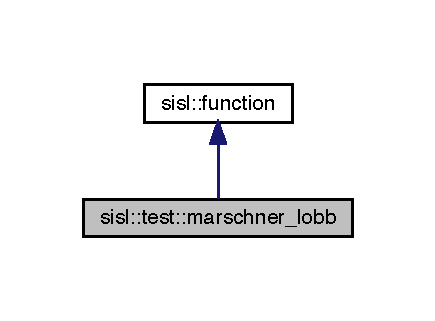
\includegraphics[width=209pt]{classsisl_1_1test_1_1marschner__lobb__inherit__graph}
\end{center}
\end{figure}


Collaboration diagram for sisl\+:\+:test\+:\+:marschner\+\_\+lobb\+:\nopagebreak
\begin{figure}[H]
\begin{center}
\leavevmode
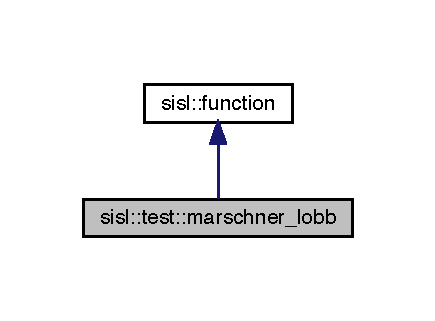
\includegraphics[width=209pt]{classsisl_1_1test_1_1marschner__lobb__coll__graph}
\end{center}
\end{figure}
\subsection*{Public Member Functions}
\begin{DoxyCompactItemize}
\item 
\hyperlink{classsisl_1_1test_1_1marschner__lobb_a48a8f4116a2e924820417b0191864e20}{marschner\+\_\+lobb} (const double \&alpha, const double \&f\+\_\+m)
\item 
\mbox{\Hypertarget{classsisl_1_1test_1_1marschner__lobb_ae605ec65e01a2692f365d73bb7135762}\label{classsisl_1_1test_1_1marschner__lobb_ae605ec65e01a2692f365d73bb7135762}} 
virtual const double \hyperlink{classsisl_1_1test_1_1marschner__lobb_ae605ec65e01a2692f365d73bb7135762}{operator()} (double d0,...) const
\begin{DoxyCompactList}\small\item\em Evaluate the function at a point. \end{DoxyCompactList}\item 
\mbox{\Hypertarget{classsisl_1_1test_1_1marschner__lobb_a04d85ffd109440215b2f77b70e24d5d5}\label{classsisl_1_1test_1_1marschner__lobb_a04d85ffd109440215b2f77b70e24d5d5}} 
virtual const double \hyperlink{classsisl_1_1test_1_1marschner__lobb_a04d85ffd109440215b2f77b70e24d5d5}{operator()} (const \hyperlink{namespacesisl_a2069bd5374a9be042ff3ce3306d41e1a}{vector} \&p) const
\begin{DoxyCompactList}\small\item\em Evaluate the function at a point. \end{DoxyCompactList}\item 
\mbox{\Hypertarget{classsisl_1_1test_1_1marschner__lobb_aa84fac794caf4cc188ac547e274648d3}\label{classsisl_1_1test_1_1marschner__lobb_aa84fac794caf4cc188ac547e274648d3}} 
virtual const double \hyperlink{classsisl_1_1test_1_1marschner__lobb_aa84fac794caf4cc188ac547e274648d3}{d} (int component, double d0,...) const
\begin{DoxyCompactList}\small\item\em Evaluate the function at a point. \end{DoxyCompactList}\item 
\mbox{\Hypertarget{classsisl_1_1test_1_1marschner__lobb_a8b2a2e637443cb4998f71d8721f9b4e2}\label{classsisl_1_1test_1_1marschner__lobb_a8b2a2e637443cb4998f71d8721f9b4e2}} 
virtual const double \hyperlink{classsisl_1_1test_1_1marschner__lobb_a8b2a2e637443cb4998f71d8721f9b4e2}{d} (int component, const \hyperlink{namespacesisl_a2069bd5374a9be042ff3ce3306d41e1a}{vector} \&p) const
\begin{DoxyCompactList}\small\item\em Evaluate the function at a point. \end{DoxyCompactList}\item 
\mbox{\Hypertarget{classsisl_1_1test_1_1marschner__lobb_a23d7487d7fb21f04365c9c482519e781}\label{classsisl_1_1test_1_1marschner__lobb_a23d7487d7fb21f04365c9c482519e781}} 
virtual const \hyperlink{namespacesisl_a2069bd5374a9be042ff3ce3306d41e1a}{vector} \hyperlink{classsisl_1_1test_1_1marschner__lobb_a23d7487d7fb21f04365c9c482519e781}{grad} (double d0,...) const
\begin{DoxyCompactList}\small\item\em Evaluate the gradient of the function at a point. \end{DoxyCompactList}\item 
\mbox{\Hypertarget{classsisl_1_1test_1_1marschner__lobb_ac2465a99b86948283dbe82050f516095}\label{classsisl_1_1test_1_1marschner__lobb_ac2465a99b86948283dbe82050f516095}} 
virtual const \hyperlink{namespacesisl_a2069bd5374a9be042ff3ce3306d41e1a}{vector} \hyperlink{classsisl_1_1test_1_1marschner__lobb_ac2465a99b86948283dbe82050f516095}{grad} (const \hyperlink{namespacesisl_a2069bd5374a9be042ff3ce3306d41e1a}{vector} \&p) const
\begin{DoxyCompactList}\small\item\em Evaluate the gradient of the function at a point. \end{DoxyCompactList}\item 
\mbox{\Hypertarget{classsisl_1_1test_1_1marschner__lobb_a0c7654dca8b2c4d496cad1b843b23edd}\label{classsisl_1_1test_1_1marschner__lobb_a0c7654dca8b2c4d496cad1b843b23edd}} 
virtual const double \hyperlink{classsisl_1_1test_1_1marschner__lobb_a0c7654dca8b2c4d496cad1b843b23edd}{n\+\_\+d} (const \hyperlink{namespacesisl_adc492e1c166a136d08b283394d81cd71}{int\+\_\+tuple} \&order, double d0,...) const
\begin{DoxyCompactList}\small\item\em Evaluate the n\textquotesingle{}th partial derivative at a point. \end{DoxyCompactList}\item 
\mbox{\Hypertarget{classsisl_1_1test_1_1marschner__lobb_aa0d1537a06ec9c5a6c5bf9148ca29b8e}\label{classsisl_1_1test_1_1marschner__lobb_aa0d1537a06ec9c5a6c5bf9148ca29b8e}} 
virtual const double \hyperlink{classsisl_1_1test_1_1marschner__lobb_aa0d1537a06ec9c5a6c5bf9148ca29b8e}{n\+\_\+d} (const \hyperlink{namespacesisl_adc492e1c166a136d08b283394d81cd71}{int\+\_\+tuple} \&order, \hyperlink{namespacesisl_a2069bd5374a9be042ff3ce3306d41e1a}{vector} \&p) const
\begin{DoxyCompactList}\small\item\em Evaluate the n\textquotesingle{}th partial derivative at a point. \end{DoxyCompactList}\item 
\mbox{\Hypertarget{classsisl_1_1test_1_1marschner__lobb_af1cd7b28be67f9078d3aff92cf32f054}\label{classsisl_1_1test_1_1marschner__lobb_af1cd7b28be67f9078d3aff92cf32f054}} 
virtual const int \hyperlink{classsisl_1_1test_1_1marschner__lobb_af1cd7b28be67f9078d3aff92cf32f054}{dim} () const
\begin{DoxyCompactList}\small\item\em Returns the input dimension of this function. \end{DoxyCompactList}\end{DoxyCompactItemize}


\subsection{Detailed Description}
Marschner lobb test function. 

\subsection{Constructor \& Destructor Documentation}
\mbox{\Hypertarget{classsisl_1_1test_1_1marschner__lobb_a48a8f4116a2e924820417b0191864e20}\label{classsisl_1_1test_1_1marschner__lobb_a48a8f4116a2e924820417b0191864e20}} 
\index{sisl\+::test\+::marschner\+\_\+lobb@{sisl\+::test\+::marschner\+\_\+lobb}!marschner\+\_\+lobb@{marschner\+\_\+lobb}}
\index{marschner\+\_\+lobb@{marschner\+\_\+lobb}!sisl\+::test\+::marschner\+\_\+lobb@{sisl\+::test\+::marschner\+\_\+lobb}}
\subsubsection{\texorpdfstring{marschner\+\_\+lobb()}{marschner\_lobb()}}
{\footnotesize\ttfamily sisl\+::test\+::marschner\+\_\+lobb\+::marschner\+\_\+lobb (\begin{DoxyParamCaption}\item[{const double \&}]{alpha,  }\item[{const double \&}]{f\+\_\+m }\end{DoxyParamCaption})\hspace{0.3cm}{\ttfamily [inline]}}

Constructor Constructs an instance of the Marshcner lobb function 
\begin{DoxyParams}{Parameters}
{\em } & \\
\hline
\end{DoxyParams}


The documentation for this class was generated from the following file\+:\begin{DoxyCompactItemize}
\item 
/\+Users/joshuahoracsek/\+Projects/sisl\+\_\+redux/include/sisl/test/function/marschner\+\_\+lobb.\+hpp\end{DoxyCompactItemize}

\hypertarget{classsisl_1_1nearest__neighbor}{}\section{sisl\+:\+:nearest\+\_\+neighbor Class Reference}
\label{classsisl_1_1nearest__neighbor}\index{sisl\+::nearest\+\_\+neighbor@{sisl\+::nearest\+\_\+neighbor}}


Nearest neighbor interpolation for any lattice. Simply finds the nearest lattice site and returns the value at that site. This class doesn\textquotesingle{}t implement phi or dphi functions, as one would need to know the lattice a-\/priori for those, and this class structure isn\textquotesingle{}t sophisticated enough to facilitate that.  




{\ttfamily \#include $<$nearest\+\_\+neighbor.\+hpp$>$}



Inheritance diagram for sisl\+:\+:nearest\+\_\+neighbor\+:\nopagebreak
\begin{figure}[H]
\begin{center}
\leavevmode
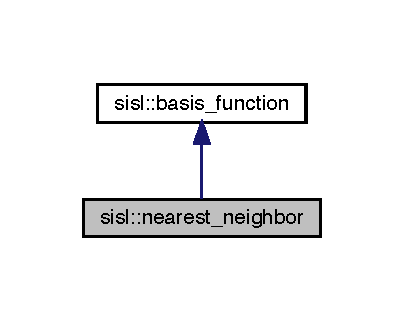
\includegraphics[width=194pt]{classsisl_1_1nearest__neighbor__inherit__graph}
\end{center}
\end{figure}


Collaboration diagram for sisl\+:\+:nearest\+\_\+neighbor\+:\nopagebreak
\begin{figure}[H]
\begin{center}
\leavevmode
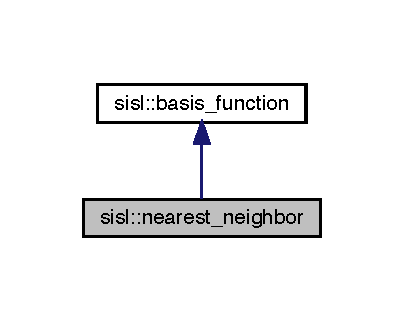
\includegraphics[width=194pt]{classsisl_1_1nearest__neighbor__coll__graph}
\end{center}
\end{figure}
\subsection*{Static Public Member Functions}
\begin{DoxyCompactItemize}
\item 
\mbox{\Hypertarget{classsisl_1_1nearest__neighbor_a14896b09eaa15503259f77e37e49cb6a}\label{classsisl_1_1nearest__neighbor_a14896b09eaa15503259f77e37e49cb6a}} 
{\footnotesize template$<$int N$>$ }\\static const double \hyperlink{classsisl_1_1nearest__neighbor_a14896b09eaa15503259f77e37e49cb6a}{phi} (const \hyperlink{namespacesisl_a2069bd5374a9be042ff3ce3306d41e1a}{vector} \&)
\begin{DoxyCompactList}\small\item\em Evaluates the un-\/scaled basis function. Evaluates the basis function as if it were not scaled by any scaling parameter. \end{DoxyCompactList}\item 
\mbox{\Hypertarget{classsisl_1_1nearest__neighbor_aced35f861bd3310d2e171fb63a6144b8}\label{classsisl_1_1nearest__neighbor_aced35f861bd3310d2e171fb63a6144b8}} 
{\footnotesize template$<$int N$>$ }\\static const double \hyperlink{classsisl_1_1nearest__neighbor_aced35f861bd3310d2e171fb63a6144b8}{phi} (const double \&h, const \hyperlink{namespacesisl_a2069bd5374a9be042ff3ce3306d41e1a}{vector} \&p)
\begin{DoxyCompactList}\small\item\em Evaluates the un-\/scaled basis function. Evaluates the basis function as if it were not scaled by any scaling parameter. This, however, does take a scale parameter, as the basis may change per scale (e.\+g. exponential splines) \end{DoxyCompactList}\item 
\mbox{\Hypertarget{classsisl_1_1nearest__neighbor_a52533a8b0e380490bbaac09f2d3292bc}\label{classsisl_1_1nearest__neighbor_a52533a8b0e380490bbaac09f2d3292bc}} 
{\footnotesize template$<$int N$>$ }\\static const double \hyperlink{classsisl_1_1nearest__neighbor_a52533a8b0e380490bbaac09f2d3292bc}{dphi} (const \hyperlink{namespacesisl_a2069bd5374a9be042ff3ce3306d41e1a}{vector} \&p, const int \&d)
\begin{DoxyCompactList}\small\item\em Evaluates the derivative of an un-\/scaled basis function. Evaluates the derivative of a basis function as if it were not scaled by any scaling parameter. \end{DoxyCompactList}\item 
\mbox{\Hypertarget{classsisl_1_1nearest__neighbor_a7adbe25f4f09abbd366053c673a8e716}\label{classsisl_1_1nearest__neighbor_a7adbe25f4f09abbd366053c673a8e716}} 
{\footnotesize template$<$int N$>$ }\\static const double \hyperlink{classsisl_1_1nearest__neighbor_a7adbe25f4f09abbd366053c673a8e716}{dphi} (const double \&h, const \hyperlink{namespacesisl_a2069bd5374a9be042ff3ce3306d41e1a}{vector} \&p, const int \&d)
\begin{DoxyCompactList}\small\item\em Evaluates the derivative of the un-\/scaled basis function. Evaluates the basis function as if it were not scaled by any scaling parameter. This, however, does take a scale parameter, as the basis may change per scale (e.\+g. exponential splines) \end{DoxyCompactList}\item 
\mbox{\Hypertarget{classsisl_1_1nearest__neighbor_ad71cd45c3d0e315b2abe2f14dbd374b3}\label{classsisl_1_1nearest__neighbor_ad71cd45c3d0e315b2abe2f14dbd374b3}} 
{\footnotesize template$<$int N$>$ }\\static std\+::vector$<$ \hyperlink{namespacesisl_acd18feee4026583db6185df2b25434aa}{lattice\+\_\+site} $>$ {\bfseries get\+\_\+integer\+\_\+support} ()
\item 
\mbox{\Hypertarget{classsisl_1_1nearest__neighbor_ac1c8bef20acdb2ef8a457d4e7a3176cd}\label{classsisl_1_1nearest__neighbor_ac1c8bef20acdb2ef8a457d4e7a3176cd}} 
static bool {\bfseries has\+\_\+derivative} ()
\item 
\mbox{\Hypertarget{classsisl_1_1nearest__neighbor_a00058ae6c642d6a1a64d7e21db24bdab}\label{classsisl_1_1nearest__neighbor_a00058ae6c642d6a1a64d7e21db24bdab}} 
{\footnotesize template$<$int N, class L , class BF $>$ }\\static double {\bfseries convolution\+\_\+sum} (const \hyperlink{namespacesisl_a2069bd5374a9be042ff3ce3306d41e1a}{vector} \&p, const L $\ast$lattice)
\item 
\mbox{\Hypertarget{classsisl_1_1nearest__neighbor_ae846be683699e686abc143008a072b95}\label{classsisl_1_1nearest__neighbor_ae846be683699e686abc143008a072b95}} 
{\footnotesize template$<$int N, class L , class BF $>$ }\\static double {\bfseries convolution\+\_\+sum\+\_\+deriv} (const \hyperlink{namespacesisl_a2069bd5374a9be042ff3ce3306d41e1a}{vector} \&p, const L $\ast$lattice, const int \&component)
\item 
\mbox{\Hypertarget{classsisl_1_1nearest__neighbor_aa765cd2944d9d5262c8f3f8c10a0dca1}\label{classsisl_1_1nearest__neighbor_aa765cd2944d9d5262c8f3f8c10a0dca1}} 
{\footnotesize template$<$int N, class L , class BF $>$ }\\static \hyperlink{namespacesisl_a2069bd5374a9be042ff3ce3306d41e1a}{vector} {\bfseries grad\+\_\+convolution\+\_\+sum} (const \hyperlink{namespacesisl_a2069bd5374a9be042ff3ce3306d41e1a}{vector} \&p, const L $\ast$lattice)
\item 
\mbox{\Hypertarget{classsisl_1_1nearest__neighbor_a0664ce6f5183fe3bcdf4397523bb9956}\label{classsisl_1_1nearest__neighbor_a0664ce6f5183fe3bcdf4397523bb9956}} 
{\footnotesize template$<$int N, class L , class BF $>$ }\\static \hyperlink{namespacesisl_a2069bd5374a9be042ff3ce3306d41e1a}{vector} {\bfseries grad\+\_\+convolution\+\_\+sum} (const \hyperlink{namespacesisl_a2069bd5374a9be042ff3ce3306d41e1a}{vector} \&p, const L $\ast$base, const L $\ast$$\ast$lattices)
\item 
\mbox{\Hypertarget{classsisl_1_1nearest__neighbor_a879c49cd3b642c8ddc5d5da4426b0e7f}\label{classsisl_1_1nearest__neighbor_a879c49cd3b642c8ddc5d5da4426b0e7f}} 
{\footnotesize template$<$int N, class L , class BF $>$ }\\static double {\bfseries convolution\+\_\+sum\+\_\+h} (const \hyperlink{namespacesisl_a2069bd5374a9be042ff3ce3306d41e1a}{vector} \&p, const L $\ast$lattice, const double \&h)
\item 
\mbox{\Hypertarget{classsisl_1_1nearest__neighbor_a5f13e5fd3eee54b8005a6398bae01ef4}\label{classsisl_1_1nearest__neighbor_a5f13e5fd3eee54b8005a6398bae01ef4}} 
{\footnotesize template$<$int N, class L , class BF $>$ }\\static double {\bfseries convolution\+\_\+sum\+\_\+deriv\+\_\+h} (const \hyperlink{namespacesisl_a2069bd5374a9be042ff3ce3306d41e1a}{vector} \&p, const L $\ast$lattice, const double \&h, const int \&component)
\item 
\mbox{\Hypertarget{classsisl_1_1nearest__neighbor_a704a5a15db9d47c51137d384c1bdbeef}\label{classsisl_1_1nearest__neighbor_a704a5a15db9d47c51137d384c1bdbeef}} 
{\footnotesize template$<$int N, class L , class BF $>$ }\\static \hyperlink{namespacesisl_a2069bd5374a9be042ff3ce3306d41e1a}{vector} {\bfseries grad\+\_\+convolution\+\_\+sum\+\_\+h} (const \hyperlink{namespacesisl_a2069bd5374a9be042ff3ce3306d41e1a}{vector} \&p, const L $\ast$lattice, const double \&h)
\item 
\mbox{\Hypertarget{classsisl_1_1nearest__neighbor_a75d7b379c635661c35fafd06b8482b89}\label{classsisl_1_1nearest__neighbor_a75d7b379c635661c35fafd06b8482b89}} 
{\footnotesize template$<$int N, class L , class BF $>$ }\\static \hyperlink{namespacesisl_a2069bd5374a9be042ff3ce3306d41e1a}{vector} {\bfseries grad\+\_\+convolution\+\_\+sum\+\_\+h} (const \hyperlink{namespacesisl_a2069bd5374a9be042ff3ce3306d41e1a}{vector} \&p, const L $\ast$base, const L $\ast$$\ast$lattices, const double \&h)
\end{DoxyCompactItemize}


\subsection{Detailed Description}
Nearest neighbor interpolation for any lattice. Simply finds the nearest lattice site and returns the value at that site. This class doesn\textquotesingle{}t implement phi or dphi functions, as one would need to know the lattice a-\/priori for those, and this class structure isn\textquotesingle{}t sophisticated enough to facilitate that. 

The documentation for this class was generated from the following file\+:\begin{DoxyCompactItemize}
\item 
/\+Users/joshuahoracsek/\+Projects/sisl\+\_\+redux/include/sisl/basis/nearest\+\_\+neighbor.\+hpp\end{DoxyCompactItemize}

\hypertarget{structsisl_1_1plane}{}\section{sisl\+:\+:plane Struct Reference}
\label{structsisl_1_1plane}\index{sisl\+::plane@{sisl\+::plane}}


3D plane class.  




{\ttfamily \#include $<$primitives.\+hpp$>$}

\subsection*{Public Member Functions}
\begin{DoxyCompactItemize}
\item 
\hyperlink{structsisl_1_1plane_af0b08037a91ded2c568f2a5d99418143}{plane} (const \hyperlink{namespacesisl_a2069bd5374a9be042ff3ce3306d41e1a}{vector} \&\+\_\+n, const sisl\+\_\+float \&\+\_\+d)
\item 
\hyperlink{structsisl_1_1plane_a6eea6dde0d9235a1afd383f98cfacec7}{plane} (const \hyperlink{structsisl_1_1plane}{plane} \&\+\_\+p)
\end{DoxyCompactItemize}
\subsection*{Public Attributes}
\begin{DoxyCompactItemize}
\item 
\mbox{\Hypertarget{structsisl_1_1plane_abbc8429614751645cc8d3eb5968926f7}\label{structsisl_1_1plane_abbc8429614751645cc8d3eb5968926f7}} 
\hyperlink{namespacesisl_a2069bd5374a9be042ff3ce3306d41e1a}{vector} \hyperlink{structsisl_1_1plane_abbc8429614751645cc8d3eb5968926f7}{n}
\begin{DoxyCompactList}\small\item\em normal direction \end{DoxyCompactList}\item 
\mbox{\Hypertarget{structsisl_1_1plane_a6eadb141c9042a48ec96577869668528}\label{structsisl_1_1plane_a6eadb141c9042a48ec96577869668528}} 
sisl\+\_\+float \hyperlink{structsisl_1_1plane_a6eadb141c9042a48ec96577869668528}{d}
\begin{DoxyCompactList}\small\item\em normal offset \end{DoxyCompactList}\end{DoxyCompactItemize}


\subsection{Detailed Description}
3D plane class. 

A plain plane class. 

\subsection{Constructor \& Destructor Documentation}
\mbox{\Hypertarget{structsisl_1_1plane_af0b08037a91ded2c568f2a5d99418143}\label{structsisl_1_1plane_af0b08037a91ded2c568f2a5d99418143}} 
\index{sisl\+::plane@{sisl\+::plane}!plane@{plane}}
\index{plane@{plane}!sisl\+::plane@{sisl\+::plane}}
\subsubsection{\texorpdfstring{plane()}{plane()}\hspace{0.1cm}{\footnotesize\ttfamily [1/2]}}
{\footnotesize\ttfamily sisl\+::plane\+::plane (\begin{DoxyParamCaption}\item[{const \hyperlink{namespacesisl_a2069bd5374a9be042ff3ce3306d41e1a}{vector} \&}]{\+\_\+n,  }\item[{const sisl\+\_\+float \&}]{\+\_\+d }\end{DoxyParamCaption})\hspace{0.3cm}{\ttfamily [inline]}}

Plane constructor 
\begin{DoxyParams}{Parameters}
{\em \+\_\+n} & Input normal direction (note, this will get normalized on assignment). \\
\hline
{\em \+\_\+d} & Input normal offset. \\
\hline
\end{DoxyParams}
\mbox{\Hypertarget{structsisl_1_1plane_a6eea6dde0d9235a1afd383f98cfacec7}\label{structsisl_1_1plane_a6eea6dde0d9235a1afd383f98cfacec7}} 
\index{sisl\+::plane@{sisl\+::plane}!plane@{plane}}
\index{plane@{plane}!sisl\+::plane@{sisl\+::plane}}
\subsubsection{\texorpdfstring{plane()}{plane()}\hspace{0.1cm}{\footnotesize\ttfamily [2/2]}}
{\footnotesize\ttfamily sisl\+::plane\+::plane (\begin{DoxyParamCaption}\item[{const \hyperlink{structsisl_1_1plane}{plane} \&}]{\+\_\+p }\end{DoxyParamCaption})\hspace{0.3cm}{\ttfamily [inline]}}

Plane copy constructor 
\begin{DoxyParams}{Parameters}
{\em \+\_\+p} & A plane to copy \\
\hline
\end{DoxyParams}


The documentation for this struct was generated from the following file\+:\begin{DoxyCompactItemize}
\item 
/\+Users/joshuahoracsek/\+Projects/sisl\+\_\+redux/include/sisl/primitives.\+hpp\end{DoxyCompactItemize}

\hypertarget{classsisl_1_1utility_1_1ply__mesh}{}\section{sisl\+:\+:utility\+:\+:ply\+\_\+mesh Class Reference}
\label{classsisl_1_1utility_1_1ply__mesh}\index{sisl\+::utility\+::ply\+\_\+mesh@{sisl\+::utility\+::ply\+\_\+mesh}}


A barebones ply mesh writer.  




{\ttfamily \#include $<$ply\+\_\+mesh.\+hpp$>$}

\subsection*{Public Member Functions}
\begin{DoxyCompactItemize}
\item 
\mbox{\Hypertarget{classsisl_1_1utility_1_1ply__mesh_ae9183ada87112161dd0a77b69ab7ce40}\label{classsisl_1_1utility_1_1ply__mesh_ae9183ada87112161dd0a77b69ab7ce40}} 
\hyperlink{classsisl_1_1utility_1_1ply__mesh_ae9183ada87112161dd0a77b69ab7ce40}{ply\+\_\+mesh} ()
\begin{DoxyCompactList}\small\item\em Create an empty mesh. \end{DoxyCompactList}\item 
int \hyperlink{classsisl_1_1utility_1_1ply__mesh_a133740c648ea0dfcc71b79f0c4737ca4}{add\+\_\+vertex} (const \hyperlink{structsisl_1_1vertex3}{vertex3} \&p)
\item 
\mbox{\Hypertarget{classsisl_1_1utility_1_1ply__mesh_a6ebea0a3ed87fc61bac43905cbf6433a}\label{classsisl_1_1utility_1_1ply__mesh_a6ebea0a3ed87fc61bac43905cbf6433a}} 
\hyperlink{namespacesisl_a2069bd5374a9be042ff3ce3306d41e1a}{sisl\+::vector} {\bfseries get\+\_\+vertex\+\_\+pos} (const unsigned int \&index)
\item 
\mbox{\Hypertarget{classsisl_1_1utility_1_1ply__mesh_a1c2ac4284e2a45d601e1f9d504fc9955}\label{classsisl_1_1utility_1_1ply__mesh_a1c2ac4284e2a45d601e1f9d504fc9955}} 
void {\bfseries set\+\_\+normal} (const unsigned int \&index, const \hyperlink{namespacesisl_a2069bd5374a9be042ff3ce3306d41e1a}{sisl\+::vector} \&normal)
\item 
int \hyperlink{classsisl_1_1utility_1_1ply__mesh_a70f823f9e4642b7bd58af145c097cfb3}{add\+\_\+triangle} (\hyperlink{structsisl_1_1vertex3}{vertex3} v1, \hyperlink{structsisl_1_1vertex3}{vertex3} v2, \hyperlink{structsisl_1_1vertex3}{vertex3} v3)
\item 
int \hyperlink{classsisl_1_1utility_1_1ply__mesh_a1cee19476c65b8f721d763116f7ed792}{add\+\_\+triangle} (int i, int j, int k)
\item 
void \hyperlink{classsisl_1_1utility_1_1ply__mesh_ae7b3db5e9e4d147f8b9c971691b416eb}{transform\+\_\+mesh} (const \hyperlink{namespacesisl_a2ef12d285ca3e626c05abbdec1f8a679}{transform} \&t)
\item 
int \hyperlink{classsisl_1_1utility_1_1ply__mesh_a4deac3d136ba76fface8b15fa3446728}{count\+\_\+vertices} ()
\item 
int \hyperlink{classsisl_1_1utility_1_1ply__mesh_a0457bbece84efba494f74b4b7bb87d82}{count\+\_\+faces} ()
\item 
\mbox{\Hypertarget{classsisl_1_1utility_1_1ply__mesh_aca9982449cf061ef0938f5435d577771}\label{classsisl_1_1utility_1_1ply__mesh_aca9982449cf061ef0938f5435d577771}} 
void {\bfseries remove\+\_\+duplicate\+\_\+vertices} ()
\item 
bool \hyperlink{classsisl_1_1utility_1_1ply__mesh_a4fce9e2a1f3d81b2243465d305164205}{write} (const std\+::string \&out) const
\end{DoxyCompactItemize}


\subsection{Detailed Description}
A barebones ply mesh writer. 

\subsection{Member Function Documentation}
\mbox{\Hypertarget{classsisl_1_1utility_1_1ply__mesh_a70f823f9e4642b7bd58af145c097cfb3}\label{classsisl_1_1utility_1_1ply__mesh_a70f823f9e4642b7bd58af145c097cfb3}} 
\index{sisl\+::utility\+::ply\+\_\+mesh@{sisl\+::utility\+::ply\+\_\+mesh}!add\+\_\+triangle@{add\+\_\+triangle}}
\index{add\+\_\+triangle@{add\+\_\+triangle}!sisl\+::utility\+::ply\+\_\+mesh@{sisl\+::utility\+::ply\+\_\+mesh}}
\subsubsection{\texorpdfstring{add\+\_\+triangle()}{add\_triangle()}\hspace{0.1cm}{\footnotesize\ttfamily [1/2]}}
{\footnotesize\ttfamily int sisl\+::utility\+::ply\+\_\+mesh\+::add\+\_\+triangle (\begin{DoxyParamCaption}\item[{\hyperlink{structsisl_1_1vertex3}{vertex3}}]{v1,  }\item[{\hyperlink{structsisl_1_1vertex3}{vertex3}}]{v2,  }\item[{\hyperlink{structsisl_1_1vertex3}{vertex3}}]{v3 }\end{DoxyParamCaption})\hspace{0.3cm}{\ttfamily [inline]}}

Adds a triangle to the mesh, checking for duplicate vertices. Returns an index into the list of faces. 
\begin{DoxyParams}{Parameters}
{\em v1,v2,v3} & A vertices that form a polygon \\
\hline
\end{DoxyParams}
\mbox{\Hypertarget{classsisl_1_1utility_1_1ply__mesh_a1cee19476c65b8f721d763116f7ed792}\label{classsisl_1_1utility_1_1ply__mesh_a1cee19476c65b8f721d763116f7ed792}} 
\index{sisl\+::utility\+::ply\+\_\+mesh@{sisl\+::utility\+::ply\+\_\+mesh}!add\+\_\+triangle@{add\+\_\+triangle}}
\index{add\+\_\+triangle@{add\+\_\+triangle}!sisl\+::utility\+::ply\+\_\+mesh@{sisl\+::utility\+::ply\+\_\+mesh}}
\subsubsection{\texorpdfstring{add\+\_\+triangle()}{add\_triangle()}\hspace{0.1cm}{\footnotesize\ttfamily [2/2]}}
{\footnotesize\ttfamily int sisl\+::utility\+::ply\+\_\+mesh\+::add\+\_\+triangle (\begin{DoxyParamCaption}\item[{int}]{i,  }\item[{int}]{j,  }\item[{int}]{k }\end{DoxyParamCaption})\hspace{0.3cm}{\ttfamily [inline]}}

Adds a triangle to the mesh, checking for duplicate vertices. Returns an index into the list of faces. 
\begin{DoxyParams}{Parameters}
{\em v1,v2,v3} & Vertex indices (from add\+\_\+verte) \\
\hline
\end{DoxyParams}
\mbox{\Hypertarget{classsisl_1_1utility_1_1ply__mesh_a133740c648ea0dfcc71b79f0c4737ca4}\label{classsisl_1_1utility_1_1ply__mesh_a133740c648ea0dfcc71b79f0c4737ca4}} 
\index{sisl\+::utility\+::ply\+\_\+mesh@{sisl\+::utility\+::ply\+\_\+mesh}!add\+\_\+vertex@{add\+\_\+vertex}}
\index{add\+\_\+vertex@{add\+\_\+vertex}!sisl\+::utility\+::ply\+\_\+mesh@{sisl\+::utility\+::ply\+\_\+mesh}}
\subsubsection{\texorpdfstring{add\+\_\+vertex()}{add\_vertex()}}
{\footnotesize\ttfamily int sisl\+::utility\+::ply\+\_\+mesh\+::add\+\_\+vertex (\begin{DoxyParamCaption}\item[{const \hyperlink{structsisl_1_1vertex3}{vertex3} \&}]{p }\end{DoxyParamCaption})\hspace{0.3cm}{\ttfamily [inline]}}

Adds a vertex to the mesh. Returns an index into the list of vertices. 
\begin{DoxyParams}{Parameters}
{\em p} & A vertex \\
\hline
\end{DoxyParams}
\mbox{\Hypertarget{classsisl_1_1utility_1_1ply__mesh_a0457bbece84efba494f74b4b7bb87d82}\label{classsisl_1_1utility_1_1ply__mesh_a0457bbece84efba494f74b4b7bb87d82}} 
\index{sisl\+::utility\+::ply\+\_\+mesh@{sisl\+::utility\+::ply\+\_\+mesh}!count\+\_\+faces@{count\+\_\+faces}}
\index{count\+\_\+faces@{count\+\_\+faces}!sisl\+::utility\+::ply\+\_\+mesh@{sisl\+::utility\+::ply\+\_\+mesh}}
\subsubsection{\texorpdfstring{count\+\_\+faces()}{count\_faces()}}
{\footnotesize\ttfamily int sisl\+::utility\+::ply\+\_\+mesh\+::count\+\_\+faces (\begin{DoxyParamCaption}{ }\end{DoxyParamCaption})\hspace{0.3cm}{\ttfamily [inline]}}

Returns the number of unique faces in the mesh \mbox{\Hypertarget{classsisl_1_1utility_1_1ply__mesh_a4deac3d136ba76fface8b15fa3446728}\label{classsisl_1_1utility_1_1ply__mesh_a4deac3d136ba76fface8b15fa3446728}} 
\index{sisl\+::utility\+::ply\+\_\+mesh@{sisl\+::utility\+::ply\+\_\+mesh}!count\+\_\+vertices@{count\+\_\+vertices}}
\index{count\+\_\+vertices@{count\+\_\+vertices}!sisl\+::utility\+::ply\+\_\+mesh@{sisl\+::utility\+::ply\+\_\+mesh}}
\subsubsection{\texorpdfstring{count\+\_\+vertices()}{count\_vertices()}}
{\footnotesize\ttfamily int sisl\+::utility\+::ply\+\_\+mesh\+::count\+\_\+vertices (\begin{DoxyParamCaption}{ }\end{DoxyParamCaption})\hspace{0.3cm}{\ttfamily [inline]}}

Returns the number of unique vertices in the mesh \mbox{\Hypertarget{classsisl_1_1utility_1_1ply__mesh_ae7b3db5e9e4d147f8b9c971691b416eb}\label{classsisl_1_1utility_1_1ply__mesh_ae7b3db5e9e4d147f8b9c971691b416eb}} 
\index{sisl\+::utility\+::ply\+\_\+mesh@{sisl\+::utility\+::ply\+\_\+mesh}!transform\+\_\+mesh@{transform\+\_\+mesh}}
\index{transform\+\_\+mesh@{transform\+\_\+mesh}!sisl\+::utility\+::ply\+\_\+mesh@{sisl\+::utility\+::ply\+\_\+mesh}}
\subsubsection{\texorpdfstring{transform\+\_\+mesh()}{transform\_mesh()}}
{\footnotesize\ttfamily void sisl\+::utility\+::ply\+\_\+mesh\+::transform\+\_\+mesh (\begin{DoxyParamCaption}\item[{const \hyperlink{namespacesisl_a2ef12d285ca3e626c05abbdec1f8a679}{transform} \&}]{t }\end{DoxyParamCaption})\hspace{0.3cm}{\ttfamily [inline]}}

Transforms all vertices in the mesh according to a transformation matrix. 
\begin{DoxyParams}{Parameters}
{\em t} & A transformation matrix. \\
\hline
\end{DoxyParams}
\mbox{\Hypertarget{classsisl_1_1utility_1_1ply__mesh_a4fce9e2a1f3d81b2243465d305164205}\label{classsisl_1_1utility_1_1ply__mesh_a4fce9e2a1f3d81b2243465d305164205}} 
\index{sisl\+::utility\+::ply\+\_\+mesh@{sisl\+::utility\+::ply\+\_\+mesh}!write@{write}}
\index{write@{write}!sisl\+::utility\+::ply\+\_\+mesh@{sisl\+::utility\+::ply\+\_\+mesh}}
\subsubsection{\texorpdfstring{write()}{write()}}
{\footnotesize\ttfamily bool sisl\+::utility\+::ply\+\_\+mesh\+::write (\begin{DoxyParamCaption}\item[{const std\+::string \&}]{out }\end{DoxyParamCaption}) const\hspace{0.3cm}{\ttfamily [inline]}}

Writes this mesh to a P\+LY file, returns false if the file \textquotesingle{}out\textquotesingle{} could not be opened for writing. 
\begin{DoxyParams}{Parameters}
{\em out} & A the name of the file to output to \\
\hline
\end{DoxyParams}


The documentation for this class was generated from the following file\+:\begin{DoxyCompactItemize}
\item 
/\+Users/joshuahoracsek/\+Projects/sisl\+\_\+redux/include/sisl/utility/ply\+\_\+mesh.\+hpp\end{DoxyCompactItemize}

\hypertarget{classsisl_1_1utility_1_1ppm__image}{}\section{sisl\+:\+:utility\+:\+:ppm\+\_\+image Class Reference}
\label{classsisl_1_1utility_1_1ppm__image}\index{sisl\+::utility\+::ppm\+\_\+image@{sisl\+::utility\+::ppm\+\_\+image}}


P\+PM image writer.  




{\ttfamily \#include $<$ppm\+\_\+image.\+hpp$>$}

\subsection*{Public Member Functions}
\begin{DoxyCompactItemize}
\item 
\hyperlink{classsisl_1_1utility_1_1ppm__image_ab049aa633ce351727260eb9ca82b6a71}{ppm\+\_\+image} (const int \&width, const int \&height)
\begin{DoxyCompactList}\small\item\em Creates a new image. \end{DoxyCompactList}\item 
\hyperlink{namespacesisl_a2069bd5374a9be042ff3ce3306d41e1a}{vector} \& \hyperlink{classsisl_1_1utility_1_1ppm__image_ad2ec02b1fcc76fbaa3d4df71200e0521}{operator()} (const int \&x, const int \&y)
\begin{DoxyCompactList}\small\item\em Accessor for pixel values. \end{DoxyCompactList}\item 
void \hyperlink{classsisl_1_1utility_1_1ppm__image_a7e3ae9169fecfcd95dc8352fa4ca1c12}{reconstruct\+\_\+image} (\hyperlink{classsisl_1_1function}{function} $\ast$f, int component=-\/1, double x=0., double y=0., double extent\+\_\+x=1., double extent\+\_\+y=1.)
\begin{DoxyCompactList}\small\item\em Samples a 2D function. \end{DoxyCompactList}\item 
void \hyperlink{classsisl_1_1utility_1_1ppm__image_a2fd1c61391d4be4802be8e2af85d507c}{clamp} (const double \&min, const double \&max)
\begin{DoxyCompactList}\small\item\em Clams all values for all components between min and max. \end{DoxyCompactList}\item 
bool \hyperlink{classsisl_1_1utility_1_1ppm__image_ac84d6c79a7ea161cb0588c838994d9d0}{write} (const std\+::string \&out, bool normalize=true)
\begin{DoxyCompactList}\small\item\em Writes an image to the specified file. \end{DoxyCompactList}\end{DoxyCompactItemize}


\subsection{Detailed Description}
P\+PM image writer. 

\subsection{Constructor \& Destructor Documentation}
\mbox{\Hypertarget{classsisl_1_1utility_1_1ppm__image_ab049aa633ce351727260eb9ca82b6a71}\label{classsisl_1_1utility_1_1ppm__image_ab049aa633ce351727260eb9ca82b6a71}} 
\index{sisl\+::utility\+::ppm\+\_\+image@{sisl\+::utility\+::ppm\+\_\+image}!ppm\+\_\+image@{ppm\+\_\+image}}
\index{ppm\+\_\+image@{ppm\+\_\+image}!sisl\+::utility\+::ppm\+\_\+image@{sisl\+::utility\+::ppm\+\_\+image}}
\subsubsection{\texorpdfstring{ppm\+\_\+image()}{ppm\_image()}}
{\footnotesize\ttfamily sisl\+::utility\+::ppm\+\_\+image\+::ppm\+\_\+image (\begin{DoxyParamCaption}\item[{const int \&}]{width,  }\item[{const int \&}]{height }\end{DoxyParamCaption})\hspace{0.3cm}{\ttfamily [inline]}}



Creates a new image. 

Creates a new image with dimensions width and height. Each cell contains an rgb\+\_\+color value. 

\subsection{Member Function Documentation}
\mbox{\Hypertarget{classsisl_1_1utility_1_1ppm__image_a2fd1c61391d4be4802be8e2af85d507c}\label{classsisl_1_1utility_1_1ppm__image_a2fd1c61391d4be4802be8e2af85d507c}} 
\index{sisl\+::utility\+::ppm\+\_\+image@{sisl\+::utility\+::ppm\+\_\+image}!clamp@{clamp}}
\index{clamp@{clamp}!sisl\+::utility\+::ppm\+\_\+image@{sisl\+::utility\+::ppm\+\_\+image}}
\subsubsection{\texorpdfstring{clamp()}{clamp()}}
{\footnotesize\ttfamily void sisl\+::utility\+::ppm\+\_\+image\+::clamp (\begin{DoxyParamCaption}\item[{const double \&}]{min,  }\item[{const double \&}]{max }\end{DoxyParamCaption})\hspace{0.3cm}{\ttfamily [inline]}}



Clams all values for all components between min and max. 

Clams all values for all components between min and max. 
\begin{DoxyParams}{Parameters}
{\em min} & Minimum value, values below this are set to minimum. \\
\hline
{\em max} & Maximum value, values above this are set to maximum. \\
\hline
\end{DoxyParams}
\mbox{\Hypertarget{classsisl_1_1utility_1_1ppm__image_ad2ec02b1fcc76fbaa3d4df71200e0521}\label{classsisl_1_1utility_1_1ppm__image_ad2ec02b1fcc76fbaa3d4df71200e0521}} 
\index{sisl\+::utility\+::ppm\+\_\+image@{sisl\+::utility\+::ppm\+\_\+image}!operator()@{operator()}}
\index{operator()@{operator()}!sisl\+::utility\+::ppm\+\_\+image@{sisl\+::utility\+::ppm\+\_\+image}}
\subsubsection{\texorpdfstring{operator()()}{operator()()}}
{\footnotesize\ttfamily \hyperlink{namespacesisl_a2069bd5374a9be042ff3ce3306d41e1a}{vector}\& sisl\+::utility\+::ppm\+\_\+image\+::operator() (\begin{DoxyParamCaption}\item[{const int \&}]{x,  }\item[{const int \&}]{y }\end{DoxyParamCaption})\hspace{0.3cm}{\ttfamily [inline]}}



Accessor for pixel values. 

Accesses an R\+GB value at pixel x,y. Stored between 0 and 1, where 0 is the lowest intensity and 1 in the highest intensity. \mbox{\Hypertarget{classsisl_1_1utility_1_1ppm__image_a7e3ae9169fecfcd95dc8352fa4ca1c12}\label{classsisl_1_1utility_1_1ppm__image_a7e3ae9169fecfcd95dc8352fa4ca1c12}} 
\index{sisl\+::utility\+::ppm\+\_\+image@{sisl\+::utility\+::ppm\+\_\+image}!reconstruct\+\_\+image@{reconstruct\+\_\+image}}
\index{reconstruct\+\_\+image@{reconstruct\+\_\+image}!sisl\+::utility\+::ppm\+\_\+image@{sisl\+::utility\+::ppm\+\_\+image}}
\subsubsection{\texorpdfstring{reconstruct\+\_\+image()}{reconstruct\_image()}}
{\footnotesize\ttfamily void sisl\+::utility\+::ppm\+\_\+image\+::reconstruct\+\_\+image (\begin{DoxyParamCaption}\item[{\hyperlink{classsisl_1_1function}{function} $\ast$}]{f,  }\item[{int}]{component = {\ttfamily -\/1},  }\item[{double}]{x = {\ttfamily 0.},  }\item[{double}]{y = {\ttfamily 0.},  }\item[{double}]{extent\+\_\+x = {\ttfamily 1.},  }\item[{double}]{extent\+\_\+y = {\ttfamily 1.} }\end{DoxyParamCaption})\hspace{0.3cm}{\ttfamily [inline]}}



Samples a 2D function. 


\begin{DoxyParams}{Parameters}
{\em f} & function to sample \\
\hline
{\em component} & Component to fill, 0 = r, 1 = b, 2 = g, -\/1 = all \\
\hline
{\em x,y} & Starting position \\
\hline
{\em extent\+\_\+x,extent\+\_\+y} & Dimension of area to sample \\
\hline
\end{DoxyParams}
\mbox{\Hypertarget{classsisl_1_1utility_1_1ppm__image_ac84d6c79a7ea161cb0588c838994d9d0}\label{classsisl_1_1utility_1_1ppm__image_ac84d6c79a7ea161cb0588c838994d9d0}} 
\index{sisl\+::utility\+::ppm\+\_\+image@{sisl\+::utility\+::ppm\+\_\+image}!write@{write}}
\index{write@{write}!sisl\+::utility\+::ppm\+\_\+image@{sisl\+::utility\+::ppm\+\_\+image}}
\subsubsection{\texorpdfstring{write()}{write()}}
{\footnotesize\ttfamily bool sisl\+::utility\+::ppm\+\_\+image\+::write (\begin{DoxyParamCaption}\item[{const std\+::string \&}]{out,  }\item[{bool}]{normalize = {\ttfamily true} }\end{DoxyParamCaption})\hspace{0.3cm}{\ttfamily [inline]}}



Writes an image to the specified file. 

Writes an image to a file, if normalize is specified, values are normalized to be between 0 and 1 along each component independently.


\begin{DoxyParams}{Parameters}
{\em output} & Output ppm file. \\
\hline
{\em normalize} & Normalize components to between 0 and 1 \\
\hline
\end{DoxyParams}


The documentation for this class was generated from the following file\+:\begin{DoxyCompactItemize}
\item 
/\+Users/joshuahoracsek/\+Projects/sisl\+\_\+redux/include/sisl/utility/ppm\+\_\+image.\+hpp\end{DoxyCompactItemize}

\hypertarget{structsisl_1_1ray}{}\section{sisl\+:\+:ray Struct Reference}
\label{structsisl_1_1ray}\index{sisl\+::ray@{sisl\+::ray}}


A ray in space.  




{\ttfamily \#include $<$primitives.\+hpp$>$}

\subsection*{Public Member Functions}
\begin{DoxyCompactItemize}
\item 
\hyperlink{structsisl_1_1ray_a4a18a538fceb31b4fe52b336a0b5f78a}{ray} (const \hyperlink{namespacesisl_afaf80b1234035c1dbd3d570c96c6a63a}{point} \&\+\_\+o, const \hyperlink{namespacesisl_a2069bd5374a9be042ff3ce3306d41e1a}{vector} \&\+\_\+d)
\item 
\hyperlink{structsisl_1_1ray_a497629918619817a4f0ca31591a3382b}{ray} (const \hyperlink{structsisl_1_1ray}{ray} \&\+\_\+r)
\item 
\hyperlink{namespacesisl_afaf80b1234035c1dbd3d570c96c6a63a}{point} \hyperlink{structsisl_1_1ray_ae32b430c114c83d70ffa2a091ee6c753}{at} (const sisl\+\_\+float \&t)
\end{DoxyCompactItemize}
\subsection*{Public Attributes}
\begin{DoxyCompactItemize}
\item 
\mbox{\Hypertarget{structsisl_1_1ray_acb0bb9002b19124ac808c226ae380204}\label{structsisl_1_1ray_acb0bb9002b19124ac808c226ae380204}} 
\hyperlink{namespacesisl_afaf80b1234035c1dbd3d570c96c6a63a}{point} \hyperlink{structsisl_1_1ray_acb0bb9002b19124ac808c226ae380204}{o}
\begin{DoxyCompactList}\small\item\em ray origin \end{DoxyCompactList}\item 
\mbox{\Hypertarget{structsisl_1_1ray_a1ceb0dbf48e5d852979bbced79551d52}\label{structsisl_1_1ray_a1ceb0dbf48e5d852979bbced79551d52}} 
\hyperlink{namespacesisl_a2069bd5374a9be042ff3ce3306d41e1a}{vector} \hyperlink{structsisl_1_1ray_a1ceb0dbf48e5d852979bbced79551d52}{d}
\begin{DoxyCompactList}\small\item\em ray direction \end{DoxyCompactList}\end{DoxyCompactItemize}


\subsection{Detailed Description}
A ray in space. 

A ray class, i.\+e. a half line. 

\subsection{Constructor \& Destructor Documentation}
\mbox{\Hypertarget{structsisl_1_1ray_a4a18a538fceb31b4fe52b336a0b5f78a}\label{structsisl_1_1ray_a4a18a538fceb31b4fe52b336a0b5f78a}} 
\index{sisl\+::ray@{sisl\+::ray}!ray@{ray}}
\index{ray@{ray}!sisl\+::ray@{sisl\+::ray}}
\subsubsection{\texorpdfstring{ray()}{ray()}\hspace{0.1cm}{\footnotesize\ttfamily [1/2]}}
{\footnotesize\ttfamily sisl\+::ray\+::ray (\begin{DoxyParamCaption}\item[{const \hyperlink{namespacesisl_afaf80b1234035c1dbd3d570c96c6a63a}{point} \&}]{\+\_\+o,  }\item[{const \hyperlink{namespacesisl_a2069bd5374a9be042ff3ce3306d41e1a}{vector} \&}]{\+\_\+d }\end{DoxyParamCaption})\hspace{0.3cm}{\ttfamily [inline]}}

Ray constructor 
\begin{DoxyParams}{Parameters}
{\em \+\_\+o} & Input ray origin. \\
\hline
{\em \+\_\+d} & Input ray direction. \\
\hline
\end{DoxyParams}
\mbox{\Hypertarget{structsisl_1_1ray_a497629918619817a4f0ca31591a3382b}\label{structsisl_1_1ray_a497629918619817a4f0ca31591a3382b}} 
\index{sisl\+::ray@{sisl\+::ray}!ray@{ray}}
\index{ray@{ray}!sisl\+::ray@{sisl\+::ray}}
\subsubsection{\texorpdfstring{ray()}{ray()}\hspace{0.1cm}{\footnotesize\ttfamily [2/2]}}
{\footnotesize\ttfamily sisl\+::ray\+::ray (\begin{DoxyParamCaption}\item[{const \hyperlink{structsisl_1_1ray}{ray} \&}]{\+\_\+r }\end{DoxyParamCaption})\hspace{0.3cm}{\ttfamily [inline]}}

Ray copy constructor 
\begin{DoxyParams}{Parameters}
{\em \+\_\+r} & Ray to copy \\
\hline
\end{DoxyParams}


\subsection{Member Function Documentation}
\mbox{\Hypertarget{structsisl_1_1ray_ae32b430c114c83d70ffa2a091ee6c753}\label{structsisl_1_1ray_ae32b430c114c83d70ffa2a091ee6c753}} 
\index{sisl\+::ray@{sisl\+::ray}!at@{at}}
\index{at@{at}!sisl\+::ray@{sisl\+::ray}}
\subsubsection{\texorpdfstring{at()}{at()}}
{\footnotesize\ttfamily \hyperlink{namespacesisl_afaf80b1234035c1dbd3d570c96c6a63a}{point} sisl\+::ray\+::at (\begin{DoxyParamCaption}\item[{const sisl\+\_\+float \&}]{t }\end{DoxyParamCaption})\hspace{0.3cm}{\ttfamily [inline]}}

Returns the point at a distinance t away from the ray, travelling in the direction of the ray. 
\begin{DoxyParams}{Parameters}
{\em t} & Distance along ray from origin \\
\hline
\end{DoxyParams}


The documentation for this struct was generated from the following file\+:\begin{DoxyCompactItemize}
\item 
/\+Users/joshuahoracsek/\+Projects/sisl\+\_\+redux/include/sisl/primitives.\+hpp\end{DoxyCompactItemize}

\hypertarget{struct__fftwalloc_1_1rebind}{}\section{\+\_\+fftwalloc$<$ T $>$\+:\+:rebind$<$ U $>$ Struct Template Reference}
\label{struct__fftwalloc_1_1rebind}\index{\+\_\+fftwalloc$<$ T $>$\+::rebind$<$ U $>$@{\+\_\+fftwalloc$<$ T $>$\+::rebind$<$ U $>$}}
\subsection*{Public Types}
\begin{DoxyCompactItemize}
\item 
\mbox{\Hypertarget{struct__fftwalloc_1_1rebind_a5fab290f258bbf41f305520df4ee9340}\label{struct__fftwalloc_1_1rebind_a5fab290f258bbf41f305520df4ee9340}} 
typedef \hyperlink{class__fftwalloc}{\+\_\+fftwalloc}$<$ U $>$ {\bfseries other}
\end{DoxyCompactItemize}


The documentation for this struct was generated from the following file\+:\begin{DoxyCompactItemize}
\item 
/\+Users/joshuahoracsek/\+Projects/sisl\+\_\+redux/include/sisl/memory/fftwalloc.\+hpp\end{DoxyCompactItemize}

\hypertarget{classsisl_1_1si__function}{}\section{sisl\+:\+:si\+\_\+function$<$ L, BF, N $>$ Class Template Reference}
\label{classsisl_1_1si__function}\index{sisl\+::si\+\_\+function$<$ L, B\+F, N $>$@{sisl\+::si\+\_\+function$<$ L, B\+F, N $>$}}


Combines a lattice and a generating function.  




{\ttfamily \#include $<$si\+\_\+function.\+hpp$>$}



Inheritance diagram for sisl\+:\+:si\+\_\+function$<$ L, BF, N $>$\+:\nopagebreak
\begin{figure}[H]
\begin{center}
\leavevmode
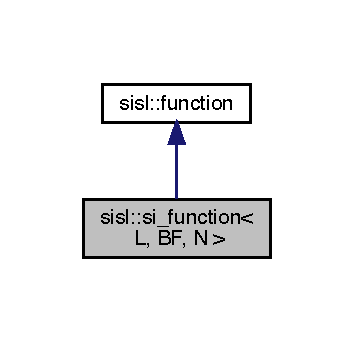
\includegraphics[width=170pt]{classsisl_1_1si__function__inherit__graph}
\end{center}
\end{figure}


Collaboration diagram for sisl\+:\+:si\+\_\+function$<$ L, BF, N $>$\+:\nopagebreak
\begin{figure}[H]
\begin{center}
\leavevmode
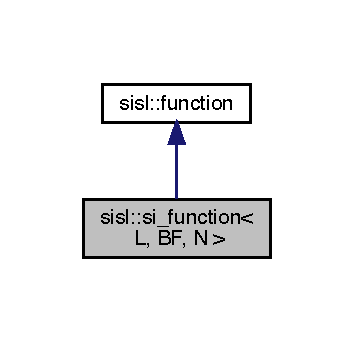
\includegraphics[width=170pt]{classsisl_1_1si__function__coll__graph}
\end{center}
\end{figure}
\subsection*{Public Member Functions}
\begin{DoxyCompactItemize}
\item 
\mbox{\Hypertarget{classsisl_1_1si__function_ae2139529aa91acee873a392fe280243d}\label{classsisl_1_1si__function_ae2139529aa91acee873a392fe280243d}} 
\hyperlink{classsisl_1_1si__function_ae2139529aa91acee873a392fe280243d}{si\+\_\+function} ()
\begin{DoxyCompactList}\small\item\em Evaluate the function at a point. \end{DoxyCompactList}\item 
\mbox{\Hypertarget{classsisl_1_1si__function_ae96061fb7b2ac6c7937728f31278e431}\label{classsisl_1_1si__function_ae96061fb7b2ac6c7937728f31278e431}} 
\hyperlink{classsisl_1_1si__function_ae96061fb7b2ac6c7937728f31278e431}{si\+\_\+function} (L $\ast$lattice)
\begin{DoxyCompactList}\small\item\em Evaluate the function at a point. \end{DoxyCompactList}\item 
\mbox{\Hypertarget{classsisl_1_1si__function_a717a52b3c4affb61b276e916d2b008d3}\label{classsisl_1_1si__function_a717a52b3c4affb61b276e916d2b008d3}} 
virtual const double \hyperlink{classsisl_1_1si__function_a717a52b3c4affb61b276e916d2b008d3}{operator()} (double d0,...) const
\begin{DoxyCompactList}\small\item\em Evaluate the function at a point. \end{DoxyCompactList}\item 
\mbox{\Hypertarget{classsisl_1_1si__function_ac273cdbf9db96a8e35ac4d6e67fae71f}\label{classsisl_1_1si__function_ac273cdbf9db96a8e35ac4d6e67fae71f}} 
virtual const double \hyperlink{classsisl_1_1si__function_ac273cdbf9db96a8e35ac4d6e67fae71f}{operator()} (const \hyperlink{namespacesisl_a2069bd5374a9be042ff3ce3306d41e1a}{vector} \&p) const
\begin{DoxyCompactList}\small\item\em Evaluate the function at a point. \end{DoxyCompactList}\item 
\mbox{\Hypertarget{classsisl_1_1si__function_acb42bd4f8b06bc38708ae2ccf8ad6b93}\label{classsisl_1_1si__function_acb42bd4f8b06bc38708ae2ccf8ad6b93}} 
virtual const double \hyperlink{classsisl_1_1si__function_acb42bd4f8b06bc38708ae2ccf8ad6b93}{d} (int component, double d0,...) const
\begin{DoxyCompactList}\small\item\em Evaluate the function at a point. \end{DoxyCompactList}\item 
\mbox{\Hypertarget{classsisl_1_1si__function_a43b958c96c151d6516e956b7187fe941}\label{classsisl_1_1si__function_a43b958c96c151d6516e956b7187fe941}} 
virtual const double \hyperlink{classsisl_1_1si__function_a43b958c96c151d6516e956b7187fe941}{d} (int component, const \hyperlink{namespacesisl_a2069bd5374a9be042ff3ce3306d41e1a}{vector} \&p) const
\begin{DoxyCompactList}\small\item\em Evaluate the function at a point. \end{DoxyCompactList}\item 
\mbox{\Hypertarget{classsisl_1_1si__function_a76031a5cf6384b8dc587ad452ed352f5}\label{classsisl_1_1si__function_a76031a5cf6384b8dc587ad452ed352f5}} 
virtual const \hyperlink{namespacesisl_a2069bd5374a9be042ff3ce3306d41e1a}{vector} \hyperlink{classsisl_1_1si__function_a76031a5cf6384b8dc587ad452ed352f5}{grad} (double d0,...) const
\begin{DoxyCompactList}\small\item\em Evaluate the function at a point. \end{DoxyCompactList}\item 
\mbox{\Hypertarget{classsisl_1_1si__function_a30f4ba2d0bdeae4c3f5738a3f4d431e4}\label{classsisl_1_1si__function_a30f4ba2d0bdeae4c3f5738a3f4d431e4}} 
virtual const \hyperlink{namespacesisl_a2069bd5374a9be042ff3ce3306d41e1a}{vector} \hyperlink{classsisl_1_1si__function_a30f4ba2d0bdeae4c3f5738a3f4d431e4}{grad} (const \hyperlink{namespacesisl_a2069bd5374a9be042ff3ce3306d41e1a}{vector} \&p) const
\begin{DoxyCompactList}\small\item\em Evaluate the function at a point. \end{DoxyCompactList}\item 
\mbox{\Hypertarget{classsisl_1_1si__function_a31d60f7c94fc37620cf543842e3ea65b}\label{classsisl_1_1si__function_a31d60f7c94fc37620cf543842e3ea65b}} 
void \hyperlink{classsisl_1_1si__function_a31d60f7c94fc37620cf543842e3ea65b}{set\+\_\+basis\+\_\+scale} (const double \&h)
\begin{DoxyCompactList}\small\item\em Sets a scale for the basis function to use. \end{DoxyCompactList}\item 
\mbox{\Hypertarget{classsisl_1_1si__function_a087ba11d61cfb8e6497d55bd66b2d180}\label{classsisl_1_1si__function_a087ba11d61cfb8e6497d55bd66b2d180}} 
void \hyperlink{classsisl_1_1si__function_a087ba11d61cfb8e6497d55bd66b2d180}{use\+\_\+basis\+\_\+gradient} ()
\begin{DoxyCompactList}\small\item\em If the basis has a derivative, this makes the function use that derivative for derivative reconstruction. \end{DoxyCompactList}\item 
\mbox{\Hypertarget{classsisl_1_1si__function_adf0831bf77e806ab9a5dc225ceaeaaed}\label{classsisl_1_1si__function_adf0831bf77e806ab9a5dc225ceaeaaed}} 
void \hyperlink{classsisl_1_1si__function_adf0831bf77e806ab9a5dc225ceaeaaed}{use\+\_\+derivative\+\_\+lattice} ()
\begin{DoxyCompactList}\small\item\em If the function has derivative lattices, this makes the function use the given basis to reconstruct derivative values. \end{DoxyCompactList}\item 
\mbox{\Hypertarget{classsisl_1_1si__function_ae012b0152662bc9e331fc668e3332729}\label{classsisl_1_1si__function_ae012b0152662bc9e331fc668e3332729}} 
void \hyperlink{classsisl_1_1si__function_ae012b0152662bc9e331fc668e3332729}{set\+\_\+lattice} (L $\ast$new\+\_\+lat)
\begin{DoxyCompactList}\small\item\em Sets the current reconstruction lattice. \end{DoxyCompactList}\item 
\mbox{\Hypertarget{classsisl_1_1si__function_a602180d6d0539667aca13b1f5d071cfc}\label{classsisl_1_1si__function_a602180d6d0539667aca13b1f5d071cfc}} 
void \hyperlink{classsisl_1_1si__function_a602180d6d0539667aca13b1f5d071cfc}{set\+\_\+derivative\+\_\+lattice} (unsigned int component, L $\ast$\hyperlink{classsisl_1_1si__function_acb42bd4f8b06bc38708ae2ccf8ad6b93}{d})
\begin{DoxyCompactList}\small\item\em Sets the lattice to be used for derivative reconstruction use \hyperlink{classsisl_1_1si__function_adf0831bf77e806ab9a5dc225ceaeaaed}{use\+\_\+derivative\+\_\+lattice()} to use this for reconstruction after all lattices have been set. \end{DoxyCompactList}\item 
\mbox{\Hypertarget{classsisl_1_1si__function_adaac36945118aaededcba9344f5be1ce}\label{classsisl_1_1si__function_adaac36945118aaededcba9344f5be1ce}} 
void \hyperlink{classsisl_1_1si__function_adaac36945118aaededcba9344f5be1ce}{set\+\_\+transform} (const \hyperlink{namespacesisl_a2ef12d285ca3e626c05abbdec1f8a679}{transform} \&t)
\begin{DoxyCompactList}\small\item\em Sets the transform for this space,. \end{DoxyCompactList}\item 
\hyperlink{namespacesisl_a2ef12d285ca3e626c05abbdec1f8a679}{transform} \hyperlink{classsisl_1_1si__function_a8e173df1adf445d4939f142846186364}{get\+\_\+transform} () const
\item 
\mbox{\Hypertarget{classsisl_1_1si__function_a717b4abb8666f883a5fd215ad356bfaf}\label{classsisl_1_1si__function_a717b4abb8666f883a5fd215ad356bfaf}} 
L $\ast$ {\bfseries get\+\_\+lattice} ()
\item 
\mbox{\Hypertarget{classsisl_1_1si__function_afa07c7ced6a5c1342e043b0f4a1faadf}\label{classsisl_1_1si__function_afa07c7ced6a5c1342e043b0f4a1faadf}} 
void {\bfseries set\+\_\+scale} (const \hyperlink{namespacesisl_a2069bd5374a9be042ff3ce3306d41e1a}{vector} \&s)
\item 
\mbox{\Hypertarget{classsisl_1_1si__function_a79b73f1edbff36dfd4f7f085b99a7e51}\label{classsisl_1_1si__function_a79b73f1edbff36dfd4f7f085b99a7e51}} 
\hyperlink{namespacesisl_a2069bd5374a9be042ff3ce3306d41e1a}{vector} {\bfseries get\+\_\+scale} () const
\item 
\mbox{\Hypertarget{classsisl_1_1si__function_aa61607a58135682c4c03062e4e77844c}\label{classsisl_1_1si__function_aa61607a58135682c4c03062e4e77844c}} 
virtual const int \hyperlink{classsisl_1_1si__function_aa61607a58135682c4c03062e4e77844c}{dim} () const
\begin{DoxyCompactList}\small\item\em Returns the input dimension of this function. \end{DoxyCompactList}\item 
\mbox{\Hypertarget{classsisl_1_1si__function_ad437132577e852410ecac53f0cab6bde}\label{classsisl_1_1si__function_ad437132577e852410ecac53f0cab6bde}} 
virtual const double \hyperlink{classsisl_1_1si__function_ad437132577e852410ecac53f0cab6bde}{n\+\_\+d} (const \hyperlink{namespacesisl_adc492e1c166a136d08b283394d81cd71}{int\+\_\+tuple} \&order, double d0,...) const
\begin{DoxyCompactList}\small\item\em Evaluate the n\textquotesingle{}th partial derivative at a point. \end{DoxyCompactList}\item 
\mbox{\Hypertarget{classsisl_1_1si__function_af7aa5368f0b296321ad1f88eb6453083}\label{classsisl_1_1si__function_af7aa5368f0b296321ad1f88eb6453083}} 
virtual const double \hyperlink{classsisl_1_1si__function_af7aa5368f0b296321ad1f88eb6453083}{n\+\_\+d} (const \hyperlink{namespacesisl_adc492e1c166a136d08b283394d81cd71}{int\+\_\+tuple} \&order, \hyperlink{namespacesisl_a2069bd5374a9be042ff3ce3306d41e1a}{vector} \&p) const
\begin{DoxyCompactList}\small\item\em Evaluate the n\textquotesingle{}th partial derivative at a point. \end{DoxyCompactList}\end{DoxyCompactItemize}


\subsection{Detailed Description}
\subsubsection*{template$<$class L, class BF, int N$>$\newline
class sisl\+::si\+\_\+function$<$ L, B\+F, N $>$}

Combines a lattice and a generating function. 



\subsection{Member Function Documentation}
\mbox{\Hypertarget{classsisl_1_1si__function_a8e173df1adf445d4939f142846186364}\label{classsisl_1_1si__function_a8e173df1adf445d4939f142846186364}} 
\index{sisl\+::si\+\_\+function@{sisl\+::si\+\_\+function}!get\+\_\+transform@{get\+\_\+transform}}
\index{get\+\_\+transform@{get\+\_\+transform}!sisl\+::si\+\_\+function@{sisl\+::si\+\_\+function}}
\subsubsection{\texorpdfstring{get\+\_\+transform()}{get\_transform()}}
{\footnotesize\ttfamily template$<$class L , class BF , int N$>$ \\
\hyperlink{namespacesisl_a2ef12d285ca3e626c05abbdec1f8a679}{transform} \hyperlink{classsisl_1_1si__function}{sisl\+::si\+\_\+function}$<$ L, BF, N $>$\+::get\+\_\+transform (\begin{DoxyParamCaption}{ }\end{DoxyParamCaption}) const\hspace{0.3cm}{\ttfamily [inline]}}

Gets the transform assiated to this space, 

The documentation for this class was generated from the following file\+:\begin{DoxyCompactItemize}
\item 
/\+Users/joshuahoracsek/\+Projects/sisl\+\_\+redux/include/sisl/function/si\+\_\+function.\+hpp\end{DoxyCompactItemize}

\hypertarget{classsisl_1_1sparse__array__n}{}\section{sisl\+:\+:sparse\+\_\+array\+\_\+n$<$ T, N, Allocator $>$ Class Template Reference}
\label{classsisl_1_1sparse__array__n}\index{sisl\+::sparse\+\_\+array\+\_\+n$<$ T, N, Allocator $>$@{sisl\+::sparse\+\_\+array\+\_\+n$<$ T, N, Allocator $>$}}


An n-\/dimensional sparese array. This class abstracts away the concept of an n-\/dimensional array, it should be easy to create an array of type T on N dimensions. It differes from an array in that, when instantiated, it consumes no memory. When you begin to fill cells of the array with data, only then does memory begin to fill up. Accessing a cell without data returns \char`\"{}default\+Value\char`\"{}, which is set in the constructor.  




{\ttfamily \#include $<$sparse\+\_\+array.\+hpp$>$}



Inheritance diagram for sisl\+:\+:sparse\+\_\+array\+\_\+n$<$ T, N, Allocator $>$\+:\nopagebreak
\begin{figure}[H]
\begin{center}
\leavevmode
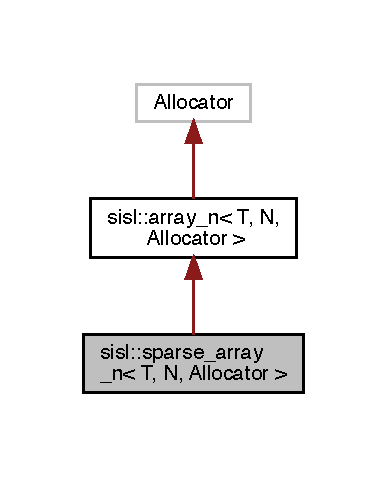
\includegraphics[width=186pt]{classsisl_1_1sparse__array__n__inherit__graph}
\end{center}
\end{figure}


Collaboration diagram for sisl\+:\+:sparse\+\_\+array\+\_\+n$<$ T, N, Allocator $>$\+:\nopagebreak
\begin{figure}[H]
\begin{center}
\leavevmode
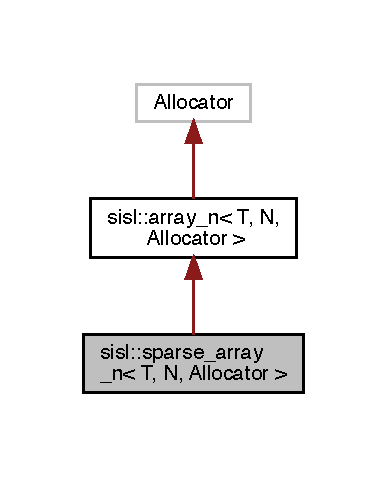
\includegraphics[width=186pt]{classsisl_1_1sparse__array__n__coll__graph}
\end{center}
\end{figure}
\subsection*{Public Member Functions}
\begin{DoxyCompactItemize}
\item 
\hyperlink{classsisl_1_1sparse__array__n_a8c957cdf94a178f0d77c1c3c374f1f91}{sparse\+\_\+array\+\_\+n} (const Allocator \&a=Allocator())
\item 
\hyperlink{classsisl_1_1sparse__array__n_afd76d3fbb0e923e2b28cfba1c675482b}{sparse\+\_\+array\+\_\+n} (const Allocator \&a, const T \&dv, unsigned int d0,...)
\item 
\hyperlink{classsisl_1_1sparse__array__n_a3132fb2f99e33ea6c34129eb1a02523f}{sparse\+\_\+array\+\_\+n} (const T \&dv, unsigned int d0,...)
\item 
\mbox{\Hypertarget{classsisl_1_1sparse__array__n_a8cffd9aaa7d7ea15fdc5071dd3ddbac7}\label{classsisl_1_1sparse__array__n_a8cffd9aaa7d7ea15fdc5071dd3ddbac7}} 
{\bfseries sparse\+\_\+array\+\_\+n} (const T \&dv, unsigned int $\ast$d)
\item 
\hyperlink{classsisl_1_1sparse__array__n_ae639c5c814a4649fcfa5ea2616e51f12}{$\sim$sparse\+\_\+array\+\_\+n} ()
\item 
unsigned int \hyperlink{classsisl_1_1sparse__array__n_a4418f97d93ce2a6cef4639ed371ee47e}{linear\+\_\+index} (unsigned int d0,...) const
\item 
unsigned int \hyperlink{classsisl_1_1sparse__array__n_a43cf90a26a41032cfc091ebb45112d13}{linear\+\_\+index} (unsigned int d0, va\+\_\+list vl) const
\item 
unsigned int \hyperlink{classsisl_1_1sparse__array__n_a39aa26464a84f3895ab34b55f5925175}{linear\+\_\+index} (unsigned int $\ast$idx) const
\item 
T \& \hyperlink{classsisl_1_1sparse__array__n_a828d9cd11de929845c584d469b4cfb0d}{operator()} (unsigned int d0,...)
\item 
const T \& \hyperlink{classsisl_1_1sparse__array__n_a37b840c55a4225232fdc8852a1a068dd}{operator()} (unsigned int d0,...) const
\item 
T \& \hyperlink{classsisl_1_1sparse__array__n_a21e3bb0965fa54371ad65e6c5cc10520}{operator()} (unsigned int $\ast$d)
\item 
const T \& \hyperlink{classsisl_1_1sparse__array__n_ad7ab70c556272a847c076ff5f3a2ad26}{operator()} (unsigned int $\ast$d) const
\item 
\mbox{\Hypertarget{classsisl_1_1sparse__array__n_a7db3ee8940017e21e3673641071f9654}\label{classsisl_1_1sparse__array__n_a7db3ee8940017e21e3673641071f9654}} 
const bool \hyperlink{classsisl_1_1sparse__array__n_a7db3ee8940017e21e3673641071f9654}{has\+\_\+value} (unsigned int d0,...) const
\begin{DoxyCompactList}\small\item\em Returns whether an index has a value For a multidimensional index, this returns whether or not that index has a value. The value at that index will always be readable, use this to know whether or not it\textquotesingle{}s a true value, or an automatically generated value. \end{DoxyCompactList}\item 
\mbox{\Hypertarget{classsisl_1_1sparse__array__n_a7fc06154d0a6c469cab565d68876e637}\label{classsisl_1_1sparse__array__n_a7fc06154d0a6c469cab565d68876e637}} 
const bool \hyperlink{classsisl_1_1sparse__array__n_a7fc06154d0a6c469cab565d68876e637}{has\+\_\+value} (unsigned int $\ast$d) const
\begin{DoxyCompactList}\small\item\em Returns whether an index has a value For a multidimensional index, this returns whether or not that index has a value. The value at that index will always be readable, use this to know whether or not it\textquotesingle{}s a true value, or an automatically generated value. \end{DoxyCompactList}\item 
\mbox{\Hypertarget{classsisl_1_1sparse__array__n_aa45b35c8068495755175df44e8b3c117}\label{classsisl_1_1sparse__array__n_aa45b35c8068495755175df44e8b3c117}} 
bool \hyperlink{classsisl_1_1sparse__array__n_aa45b35c8068495755175df44e8b3c117}{dump\+\_\+to\+\_\+stream} (std\+::ofstream \&stream) const
\begin{DoxyCompactList}\small\item\em Dumps this array to a file stream at its current index. \end{DoxyCompactList}\item 
\mbox{\Hypertarget{classsisl_1_1sparse__array__n_a76553311b73e61d9abc06b615f9997d6}\label{classsisl_1_1sparse__array__n_a76553311b73e61d9abc06b615f9997d6}} 
bool \hyperlink{classsisl_1_1sparse__array__n_a76553311b73e61d9abc06b615f9997d6}{read\+\_\+from\+\_\+stream} (std\+::ifstream \&stream)
\begin{DoxyCompactList}\small\item\em Reads data from a filestream. \end{DoxyCompactList}\end{DoxyCompactItemize}


\subsection{Detailed Description}
\subsubsection*{template$<$class T, int N, class Allocator = std\+::allocator$<$\+T$>$$>$\newline
class sisl\+::sparse\+\_\+array\+\_\+n$<$ T, N, Allocator $>$}

An n-\/dimensional sparese array. This class abstracts away the concept of an n-\/dimensional array, it should be easy to create an array of type T on N dimensions. It differes from an array in that, when instantiated, it consumes no memory. When you begin to fill cells of the array with data, only then does memory begin to fill up. Accessing a cell without data returns \char`\"{}default\+Value\char`\"{}, which is set in the constructor. 

\subsection{Constructor \& Destructor Documentation}
\mbox{\Hypertarget{classsisl_1_1sparse__array__n_a8c957cdf94a178f0d77c1c3c374f1f91}\label{classsisl_1_1sparse__array__n_a8c957cdf94a178f0d77c1c3c374f1f91}} 
\index{sisl\+::sparse\+\_\+array\+\_\+n@{sisl\+::sparse\+\_\+array\+\_\+n}!sparse\+\_\+array\+\_\+n@{sparse\+\_\+array\+\_\+n}}
\index{sparse\+\_\+array\+\_\+n@{sparse\+\_\+array\+\_\+n}!sisl\+::sparse\+\_\+array\+\_\+n@{sisl\+::sparse\+\_\+array\+\_\+n}}
\subsubsection{\texorpdfstring{sparse\+\_\+array\+\_\+n()}{sparse\_array\_n()}\hspace{0.1cm}{\footnotesize\ttfamily [1/3]}}
{\footnotesize\ttfamily template$<$class T , int N, class Allocator  = std\+::allocator$<$\+T$>$$>$ \\
\hyperlink{classsisl_1_1sparse__array__n}{sisl\+::sparse\+\_\+array\+\_\+n}$<$ T, N, Allocator $>$\+::\hyperlink{classsisl_1_1sparse__array__n}{sparse\+\_\+array\+\_\+n} (\begin{DoxyParamCaption}\item[{const Allocator \&}]{a = {\ttfamily Allocator()} }\end{DoxyParamCaption})\hspace{0.3cm}{\ttfamily [inline]}}

Default constructor. Default constructor, allocates nothing. \mbox{\Hypertarget{classsisl_1_1sparse__array__n_afd76d3fbb0e923e2b28cfba1c675482b}\label{classsisl_1_1sparse__array__n_afd76d3fbb0e923e2b28cfba1c675482b}} 
\index{sisl\+::sparse\+\_\+array\+\_\+n@{sisl\+::sparse\+\_\+array\+\_\+n}!sparse\+\_\+array\+\_\+n@{sparse\+\_\+array\+\_\+n}}
\index{sparse\+\_\+array\+\_\+n@{sparse\+\_\+array\+\_\+n}!sisl\+::sparse\+\_\+array\+\_\+n@{sisl\+::sparse\+\_\+array\+\_\+n}}
\subsubsection{\texorpdfstring{sparse\+\_\+array\+\_\+n()}{sparse\_array\_n()}\hspace{0.1cm}{\footnotesize\ttfamily [2/3]}}
{\footnotesize\ttfamily template$<$class T , int N, class Allocator  = std\+::allocator$<$\+T$>$$>$ \\
\hyperlink{classsisl_1_1sparse__array__n}{sisl\+::sparse\+\_\+array\+\_\+n}$<$ T, N, Allocator $>$\+::\hyperlink{classsisl_1_1sparse__array__n}{sparse\+\_\+array\+\_\+n} (\begin{DoxyParamCaption}\item[{const Allocator \&}]{a,  }\item[{const T \&}]{dv,  }\item[{unsigned int}]{d0,  }\item[{}]{... }\end{DoxyParamCaption})\hspace{0.3cm}{\ttfamily [inline]}}

N-\/dim constructor. Allocates an array with N dimensions with maximum dimensions given by the parameters. \mbox{\Hypertarget{classsisl_1_1sparse__array__n_a3132fb2f99e33ea6c34129eb1a02523f}\label{classsisl_1_1sparse__array__n_a3132fb2f99e33ea6c34129eb1a02523f}} 
\index{sisl\+::sparse\+\_\+array\+\_\+n@{sisl\+::sparse\+\_\+array\+\_\+n}!sparse\+\_\+array\+\_\+n@{sparse\+\_\+array\+\_\+n}}
\index{sparse\+\_\+array\+\_\+n@{sparse\+\_\+array\+\_\+n}!sisl\+::sparse\+\_\+array\+\_\+n@{sisl\+::sparse\+\_\+array\+\_\+n}}
\subsubsection{\texorpdfstring{sparse\+\_\+array\+\_\+n()}{sparse\_array\_n()}\hspace{0.1cm}{\footnotesize\ttfamily [3/3]}}
{\footnotesize\ttfamily template$<$class T , int N, class Allocator  = std\+::allocator$<$\+T$>$$>$ \\
\hyperlink{classsisl_1_1sparse__array__n}{sisl\+::sparse\+\_\+array\+\_\+n}$<$ T, N, Allocator $>$\+::\hyperlink{classsisl_1_1sparse__array__n}{sparse\+\_\+array\+\_\+n} (\begin{DoxyParamCaption}\item[{const T \&}]{dv,  }\item[{unsigned int}]{d0,  }\item[{}]{... }\end{DoxyParamCaption})\hspace{0.3cm}{\ttfamily [inline]}}

N-\/dim constructor. Allocates an array with N dimensions with maximum dimensions given by the parameters. \mbox{\Hypertarget{classsisl_1_1sparse__array__n_ae639c5c814a4649fcfa5ea2616e51f12}\label{classsisl_1_1sparse__array__n_ae639c5c814a4649fcfa5ea2616e51f12}} 
\index{sisl\+::sparse\+\_\+array\+\_\+n@{sisl\+::sparse\+\_\+array\+\_\+n}!````~sparse\+\_\+array\+\_\+n@{$\sim$sparse\+\_\+array\+\_\+n}}
\index{````~sparse\+\_\+array\+\_\+n@{$\sim$sparse\+\_\+array\+\_\+n}!sisl\+::sparse\+\_\+array\+\_\+n@{sisl\+::sparse\+\_\+array\+\_\+n}}
\subsubsection{\texorpdfstring{$\sim$sparse\+\_\+array\+\_\+n()}{~sparse\_array\_n()}}
{\footnotesize\ttfamily template$<$class T , int N, class Allocator  = std\+::allocator$<$\+T$>$$>$ \\
\hyperlink{classsisl_1_1sparse__array__n}{sisl\+::sparse\+\_\+array\+\_\+n}$<$ T, N, Allocator $>$\+::$\sim$\hyperlink{classsisl_1_1sparse__array__n}{sparse\+\_\+array\+\_\+n} (\begin{DoxyParamCaption}{ }\end{DoxyParamCaption})\hspace{0.3cm}{\ttfamily [inline]}}

N-\/dim constructor. Allocates an array with N dimensions with maximum dimensions given by the parameters. 

\subsection{Member Function Documentation}
\mbox{\Hypertarget{classsisl_1_1sparse__array__n_a4418f97d93ce2a6cef4639ed371ee47e}\label{classsisl_1_1sparse__array__n_a4418f97d93ce2a6cef4639ed371ee47e}} 
\index{sisl\+::sparse\+\_\+array\+\_\+n@{sisl\+::sparse\+\_\+array\+\_\+n}!linear\+\_\+index@{linear\+\_\+index}}
\index{linear\+\_\+index@{linear\+\_\+index}!sisl\+::sparse\+\_\+array\+\_\+n@{sisl\+::sparse\+\_\+array\+\_\+n}}
\subsubsection{\texorpdfstring{linear\+\_\+index()}{linear\_index()}\hspace{0.1cm}{\footnotesize\ttfamily [1/3]}}
{\footnotesize\ttfamily template$<$class T , int N, class Allocator  = std\+::allocator$<$\+T$>$$>$ \\
unsigned int \hyperlink{classsisl_1_1sparse__array__n}{sisl\+::sparse\+\_\+array\+\_\+n}$<$ T, N, Allocator $>$\+::linear\+\_\+index (\begin{DoxyParamCaption}\item[{unsigned int}]{d0,  }\item[{}]{... }\end{DoxyParamCaption}) const\hspace{0.3cm}{\ttfamily [inline]}}

/brief Returns a unique index for this index. This returns a unique index for a point index, this should generally be an index between 0 and max\+\_\+dim\+\_\+1$\ast$max\+\_\+dim\+\_\+2$\ast$...$\ast$max\+\_\+dim\+\_\+N -\/ 1. \mbox{\Hypertarget{classsisl_1_1sparse__array__n_a43cf90a26a41032cfc091ebb45112d13}\label{classsisl_1_1sparse__array__n_a43cf90a26a41032cfc091ebb45112d13}} 
\index{sisl\+::sparse\+\_\+array\+\_\+n@{sisl\+::sparse\+\_\+array\+\_\+n}!linear\+\_\+index@{linear\+\_\+index}}
\index{linear\+\_\+index@{linear\+\_\+index}!sisl\+::sparse\+\_\+array\+\_\+n@{sisl\+::sparse\+\_\+array\+\_\+n}}
\subsubsection{\texorpdfstring{linear\+\_\+index()}{linear\_index()}\hspace{0.1cm}{\footnotesize\ttfamily [2/3]}}
{\footnotesize\ttfamily template$<$class T , int N, class Allocator  = std\+::allocator$<$\+T$>$$>$ \\
unsigned int \hyperlink{classsisl_1_1sparse__array__n}{sisl\+::sparse\+\_\+array\+\_\+n}$<$ T, N, Allocator $>$\+::linear\+\_\+index (\begin{DoxyParamCaption}\item[{unsigned int}]{d0,  }\item[{va\+\_\+list}]{vl }\end{DoxyParamCaption}) const\hspace{0.3cm}{\ttfamily [inline]}}

/brief Returns a unique index for this index. This returns a unique index for a point index, this should generally be an index between 0 and max\+\_\+dim\+\_\+1$\ast$max\+\_\+dim\+\_\+2$\ast$...$\ast$max\+\_\+dim\+\_\+N -\/ 1. \mbox{\Hypertarget{classsisl_1_1sparse__array__n_a39aa26464a84f3895ab34b55f5925175}\label{classsisl_1_1sparse__array__n_a39aa26464a84f3895ab34b55f5925175}} 
\index{sisl\+::sparse\+\_\+array\+\_\+n@{sisl\+::sparse\+\_\+array\+\_\+n}!linear\+\_\+index@{linear\+\_\+index}}
\index{linear\+\_\+index@{linear\+\_\+index}!sisl\+::sparse\+\_\+array\+\_\+n@{sisl\+::sparse\+\_\+array\+\_\+n}}
\subsubsection{\texorpdfstring{linear\+\_\+index()}{linear\_index()}\hspace{0.1cm}{\footnotesize\ttfamily [3/3]}}
{\footnotesize\ttfamily template$<$class T , int N, class Allocator  = std\+::allocator$<$\+T$>$$>$ \\
unsigned int \hyperlink{classsisl_1_1sparse__array__n}{sisl\+::sparse\+\_\+array\+\_\+n}$<$ T, N, Allocator $>$\+::linear\+\_\+index (\begin{DoxyParamCaption}\item[{unsigned int $\ast$}]{idx }\end{DoxyParamCaption}) const\hspace{0.3cm}{\ttfamily [inline]}}

/brief Returns a unique index for this index. This returns a unique index for a point index, this should generally be an index between 0 and max\+\_\+dim\+\_\+1$\ast$max\+\_\+dim\+\_\+2$\ast$...$\ast$max\+\_\+dim\+\_\+N -\/ 1. \mbox{\Hypertarget{classsisl_1_1sparse__array__n_a828d9cd11de929845c584d469b4cfb0d}\label{classsisl_1_1sparse__array__n_a828d9cd11de929845c584d469b4cfb0d}} 
\index{sisl\+::sparse\+\_\+array\+\_\+n@{sisl\+::sparse\+\_\+array\+\_\+n}!operator()@{operator()}}
\index{operator()@{operator()}!sisl\+::sparse\+\_\+array\+\_\+n@{sisl\+::sparse\+\_\+array\+\_\+n}}
\subsubsection{\texorpdfstring{operator()()}{operator()()}\hspace{0.1cm}{\footnotesize\ttfamily [1/4]}}
{\footnotesize\ttfamily template$<$class T , int N, class Allocator  = std\+::allocator$<$\+T$>$$>$ \\
T\& \hyperlink{classsisl_1_1sparse__array__n}{sisl\+::sparse\+\_\+array\+\_\+n}$<$ T, N, Allocator $>$\+::operator() (\begin{DoxyParamCaption}\item[{unsigned int}]{d0,  }\item[{}]{... }\end{DoxyParamCaption})\hspace{0.3cm}{\ttfamily [inline]}}

/brief Accessor functions. Access a value in the array, returns a reference so it is possible to write to indices via this overload. \mbox{\Hypertarget{classsisl_1_1sparse__array__n_a37b840c55a4225232fdc8852a1a068dd}\label{classsisl_1_1sparse__array__n_a37b840c55a4225232fdc8852a1a068dd}} 
\index{sisl\+::sparse\+\_\+array\+\_\+n@{sisl\+::sparse\+\_\+array\+\_\+n}!operator()@{operator()}}
\index{operator()@{operator()}!sisl\+::sparse\+\_\+array\+\_\+n@{sisl\+::sparse\+\_\+array\+\_\+n}}
\subsubsection{\texorpdfstring{operator()()}{operator()()}\hspace{0.1cm}{\footnotesize\ttfamily [2/4]}}
{\footnotesize\ttfamily template$<$class T , int N, class Allocator  = std\+::allocator$<$\+T$>$$>$ \\
const T\& \hyperlink{classsisl_1_1sparse__array__n}{sisl\+::sparse\+\_\+array\+\_\+n}$<$ T, N, Allocator $>$\+::operator() (\begin{DoxyParamCaption}\item[{unsigned int}]{d0,  }\item[{}]{... }\end{DoxyParamCaption}) const\hspace{0.3cm}{\ttfamily [inline]}}

/brief Accessor functions. Access a value in the array, returns a reference so it is possible to write to indices via this overload. \mbox{\Hypertarget{classsisl_1_1sparse__array__n_a21e3bb0965fa54371ad65e6c5cc10520}\label{classsisl_1_1sparse__array__n_a21e3bb0965fa54371ad65e6c5cc10520}} 
\index{sisl\+::sparse\+\_\+array\+\_\+n@{sisl\+::sparse\+\_\+array\+\_\+n}!operator()@{operator()}}
\index{operator()@{operator()}!sisl\+::sparse\+\_\+array\+\_\+n@{sisl\+::sparse\+\_\+array\+\_\+n}}
\subsubsection{\texorpdfstring{operator()()}{operator()()}\hspace{0.1cm}{\footnotesize\ttfamily [3/4]}}
{\footnotesize\ttfamily template$<$class T , int N, class Allocator  = std\+::allocator$<$\+T$>$$>$ \\
T\& \hyperlink{classsisl_1_1sparse__array__n}{sisl\+::sparse\+\_\+array\+\_\+n}$<$ T, N, Allocator $>$\+::operator() (\begin{DoxyParamCaption}\item[{unsigned int $\ast$}]{d }\end{DoxyParamCaption})\hspace{0.3cm}{\ttfamily [inline]}}

/brief Accessor functions. Access a value in the array, returns a reference so it is possible to write to indices via this overload. \mbox{\Hypertarget{classsisl_1_1sparse__array__n_ad7ab70c556272a847c076ff5f3a2ad26}\label{classsisl_1_1sparse__array__n_ad7ab70c556272a847c076ff5f3a2ad26}} 
\index{sisl\+::sparse\+\_\+array\+\_\+n@{sisl\+::sparse\+\_\+array\+\_\+n}!operator()@{operator()}}
\index{operator()@{operator()}!sisl\+::sparse\+\_\+array\+\_\+n@{sisl\+::sparse\+\_\+array\+\_\+n}}
\subsubsection{\texorpdfstring{operator()()}{operator()()}\hspace{0.1cm}{\footnotesize\ttfamily [4/4]}}
{\footnotesize\ttfamily template$<$class T , int N, class Allocator  = std\+::allocator$<$\+T$>$$>$ \\
const T\& \hyperlink{classsisl_1_1sparse__array__n}{sisl\+::sparse\+\_\+array\+\_\+n}$<$ T, N, Allocator $>$\+::operator() (\begin{DoxyParamCaption}\item[{unsigned int $\ast$}]{d }\end{DoxyParamCaption}) const\hspace{0.3cm}{\ttfamily [inline]}}

/brief Accessor functions. Access a value in the array, returns a reference so it is possible to write to indices via this overload. 

The documentation for this class was generated from the following file\+:\begin{DoxyCompactItemize}
\item 
/\+Users/joshuahoracsek/\+Projects/sisl\+\_\+redux/include/sisl/memory/sparse\+\_\+array.\+hpp\end{DoxyCompactItemize}

\hypertarget{classsisl_1_1test_1_1test__window}{}\section{sisl\+:\+:test\+:\+:test\+\_\+window Class Reference}
\label{classsisl_1_1test_1_1test__window}\index{sisl\+::test\+::test\+\_\+window@{sisl\+::test\+::test\+\_\+window}}


Windowed test function.  




{\ttfamily \#include $<$test\+\_\+window.\+hpp$>$}



Inheritance diagram for sisl\+:\+:test\+:\+:test\+\_\+window\+:\nopagebreak
\begin{figure}[H]
\begin{center}
\leavevmode
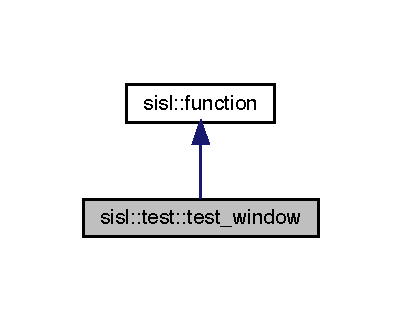
\includegraphics[width=193pt]{classsisl_1_1test_1_1test__window__inherit__graph}
\end{center}
\end{figure}


Collaboration diagram for sisl\+:\+:test\+:\+:test\+\_\+window\+:\nopagebreak
\begin{figure}[H]
\begin{center}
\leavevmode
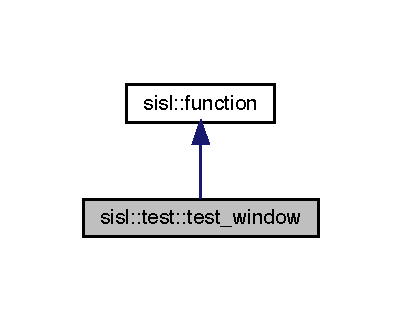
\includegraphics[width=193pt]{classsisl_1_1test_1_1test__window__coll__graph}
\end{center}
\end{figure}
\subsection*{Public Member Functions}
\begin{DoxyCompactItemize}
\item 
\mbox{\Hypertarget{classsisl_1_1test_1_1test__window_a814750884074212b92bc6e48af1b1c56}\label{classsisl_1_1test_1_1test__window_a814750884074212b92bc6e48af1b1c56}} 
{\bfseries test\+\_\+window} (const double \&alpha, const double \&gamma, const double \&f\+\_\+m)
\item 
\mbox{\Hypertarget{classsisl_1_1test_1_1test__window_a1e5ba236c8a98eda588fe418c5c44059}\label{classsisl_1_1test_1_1test__window_a1e5ba236c8a98eda588fe418c5c44059}} 
virtual const double \hyperlink{classsisl_1_1test_1_1test__window_a1e5ba236c8a98eda588fe418c5c44059}{operator()} (double d0,...) const
\begin{DoxyCompactList}\small\item\em Evaluate the function at a point. \end{DoxyCompactList}\item 
\mbox{\Hypertarget{classsisl_1_1test_1_1test__window_a136fcec74e082b51603ec34d5aecb97d}\label{classsisl_1_1test_1_1test__window_a136fcec74e082b51603ec34d5aecb97d}} 
virtual const double \hyperlink{classsisl_1_1test_1_1test__window_a136fcec74e082b51603ec34d5aecb97d}{operator()} (const \hyperlink{namespacesisl_a2069bd5374a9be042ff3ce3306d41e1a}{vector} \&p) const
\begin{DoxyCompactList}\small\item\em Evaluate the function at a point. \end{DoxyCompactList}\item 
\mbox{\Hypertarget{classsisl_1_1test_1_1test__window_a905de724a7fd4384e79788bb32443f6c}\label{classsisl_1_1test_1_1test__window_a905de724a7fd4384e79788bb32443f6c}} 
virtual const double \hyperlink{classsisl_1_1test_1_1test__window_a905de724a7fd4384e79788bb32443f6c}{d} (int component, double d0,...) const
\begin{DoxyCompactList}\small\item\em Evaluate the function at a point. \end{DoxyCompactList}\item 
\mbox{\Hypertarget{classsisl_1_1test_1_1test__window_af3d49aef2f190524c2537731bdbeb1ea}\label{classsisl_1_1test_1_1test__window_af3d49aef2f190524c2537731bdbeb1ea}} 
virtual const double \hyperlink{classsisl_1_1test_1_1test__window_af3d49aef2f190524c2537731bdbeb1ea}{d} (int component, const \hyperlink{namespacesisl_a2069bd5374a9be042ff3ce3306d41e1a}{vector} \&p) const
\begin{DoxyCompactList}\small\item\em Evaluate the function at a point. \end{DoxyCompactList}\item 
\mbox{\Hypertarget{classsisl_1_1test_1_1test__window_abb226d987d3d8d53f328ec15e6b560e3}\label{classsisl_1_1test_1_1test__window_abb226d987d3d8d53f328ec15e6b560e3}} 
virtual const \hyperlink{namespacesisl_a2069bd5374a9be042ff3ce3306d41e1a}{vector} \hyperlink{classsisl_1_1test_1_1test__window_abb226d987d3d8d53f328ec15e6b560e3}{grad} (double d0,...) const
\begin{DoxyCompactList}\small\item\em Evaluate rhe gradient of the function at a point. \end{DoxyCompactList}\item 
\mbox{\Hypertarget{classsisl_1_1test_1_1test__window_a6d0908757e3cb0a0f5d011c0f01ca264}\label{classsisl_1_1test_1_1test__window_a6d0908757e3cb0a0f5d011c0f01ca264}} 
virtual const \hyperlink{namespacesisl_a2069bd5374a9be042ff3ce3306d41e1a}{vector} \hyperlink{classsisl_1_1test_1_1test__window_a6d0908757e3cb0a0f5d011c0f01ca264}{grad} (const \hyperlink{namespacesisl_a2069bd5374a9be042ff3ce3306d41e1a}{vector} \&p) const
\begin{DoxyCompactList}\small\item\em Evaluate rhe gradient of the function at a point. \end{DoxyCompactList}\item 
\mbox{\Hypertarget{classsisl_1_1test_1_1test__window_a7ee40947015eff3a13ddac0ad3a6ef57}\label{classsisl_1_1test_1_1test__window_a7ee40947015eff3a13ddac0ad3a6ef57}} 
virtual const double \hyperlink{classsisl_1_1test_1_1test__window_a7ee40947015eff3a13ddac0ad3a6ef57}{n\+\_\+d} (const \hyperlink{namespacesisl_adc492e1c166a136d08b283394d81cd71}{int\+\_\+tuple} \&order, double d0,...) const
\begin{DoxyCompactList}\small\item\em Evaluate the n\textquotesingle{}th partial derivative at a point. \end{DoxyCompactList}\item 
\mbox{\Hypertarget{classsisl_1_1test_1_1test__window_a3240f71ac75869ad92882b4835f4fbe5}\label{classsisl_1_1test_1_1test__window_a3240f71ac75869ad92882b4835f4fbe5}} 
virtual const double \hyperlink{classsisl_1_1test_1_1test__window_a3240f71ac75869ad92882b4835f4fbe5}{n\+\_\+d} (const \hyperlink{namespacesisl_adc492e1c166a136d08b283394d81cd71}{int\+\_\+tuple} \&order, \hyperlink{namespacesisl_a2069bd5374a9be042ff3ce3306d41e1a}{vector} \&p) const
\begin{DoxyCompactList}\small\item\em Evaluate the n\textquotesingle{}th partial derivative at a point. \end{DoxyCompactList}\item 
\mbox{\Hypertarget{classsisl_1_1test_1_1test__window_ae9d16844d527e716838085ab436d1f06}\label{classsisl_1_1test_1_1test__window_ae9d16844d527e716838085ab436d1f06}} 
virtual const int \hyperlink{classsisl_1_1test_1_1test__window_ae9d16844d527e716838085ab436d1f06}{dim} () const
\begin{DoxyCompactList}\small\item\em Returns the input dimension of this function. \end{DoxyCompactList}\end{DoxyCompactItemize}


\subsection{Detailed Description}
Windowed test function. 

The documentation for this class was generated from the following file\+:\begin{DoxyCompactItemize}
\item 
/\+Users/joshuahoracsek/\+Projects/sisl\+\_\+redux/include/sisl/test/function/test\+\_\+window.\+hpp\end{DoxyCompactItemize}

\hypertarget{classsisl_1_1tp__cubic}{}\section{sisl\+:\+:tp\+\_\+cubic Class Reference}
\label{classsisl_1_1tp__cubic}\index{sisl\+::tp\+\_\+cubic@{sisl\+::tp\+\_\+cubic}}


Tensor product cubic spline.  




{\ttfamily \#include $<$tp\+\_\+cubic.\+hpp$>$}



Inheritance diagram for sisl\+:\+:tp\+\_\+cubic\+:\nopagebreak
\begin{figure}[H]
\begin{center}
\leavevmode
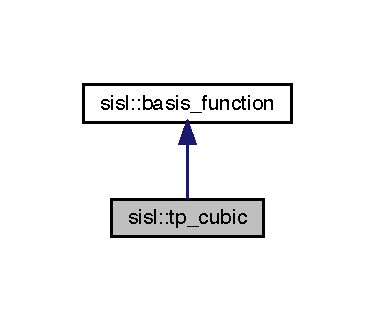
\includegraphics[width=180pt]{classsisl_1_1tp__cubic__inherit__graph}
\end{center}
\end{figure}


Collaboration diagram for sisl\+:\+:tp\+\_\+cubic\+:\nopagebreak
\begin{figure}[H]
\begin{center}
\leavevmode
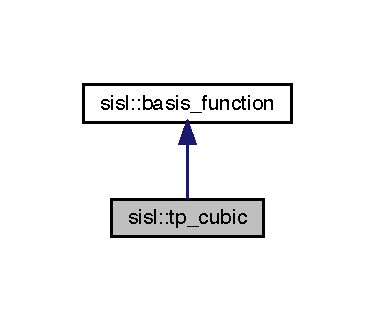
\includegraphics[width=180pt]{classsisl_1_1tp__cubic__coll__graph}
\end{center}
\end{figure}
\subsection*{Static Public Member Functions}
\begin{DoxyCompactItemize}
\item 
\mbox{\Hypertarget{classsisl_1_1tp__cubic_a717a5f75c5baff3a20142c84553f34a9}\label{classsisl_1_1tp__cubic_a717a5f75c5baff3a20142c84553f34a9}} 
{\footnotesize template$<$int N$>$ }\\static const double {\bfseries phi} (const \hyperlink{namespacesisl_a2069bd5374a9be042ff3ce3306d41e1a}{vector} \&p)
\item 
\mbox{\Hypertarget{classsisl_1_1tp__cubic_a61f057dc4599b7bf46c604d643828a7f}\label{classsisl_1_1tp__cubic_a61f057dc4599b7bf46c604d643828a7f}} 
{\footnotesize template$<$int N$>$ }\\static const double {\bfseries phi} (const double \&h, const \hyperlink{namespacesisl_a2069bd5374a9be042ff3ce3306d41e1a}{vector} \&p)
\item 
\mbox{\Hypertarget{classsisl_1_1tp__cubic_af163cd3ee7d71d4df889cb9839ba61ec}\label{classsisl_1_1tp__cubic_af163cd3ee7d71d4df889cb9839ba61ec}} 
{\footnotesize template$<$int N$>$ }\\static const double {\bfseries dphi} (const \hyperlink{namespacesisl_a2069bd5374a9be042ff3ce3306d41e1a}{vector} \&p, const int \&d)
\item 
\mbox{\Hypertarget{classsisl_1_1tp__cubic_a85b24bc94f1e152003107d2d190c7fe0}\label{classsisl_1_1tp__cubic_a85b24bc94f1e152003107d2d190c7fe0}} 
{\footnotesize template$<$int N$>$ }\\static const double {\bfseries dphi} (const double \&h, const \hyperlink{namespacesisl_a2069bd5374a9be042ff3ce3306d41e1a}{vector} \&p, const int \&d)
\item 
\mbox{\Hypertarget{classsisl_1_1tp__cubic_aa87d4d230123f3c82b5e8a0a3f5dde04}\label{classsisl_1_1tp__cubic_aa87d4d230123f3c82b5e8a0a3f5dde04}} 
{\footnotesize template$<$int N$>$ }\\static std\+::vector$<$ \hyperlink{namespacesisl_acd18feee4026583db6185df2b25434aa}{lattice\+\_\+site} $>$ {\bfseries get\+\_\+integer\+\_\+support} ()
\item 
\mbox{\Hypertarget{classsisl_1_1tp__cubic_ab4828901b48eae94fd931f1b500e767a}\label{classsisl_1_1tp__cubic_ab4828901b48eae94fd931f1b500e767a}} 
static bool {\bfseries has\+\_\+derivative} ()
\item 
\mbox{\Hypertarget{classsisl_1_1tp__cubic_a959ed13a8a900161922d9a29fce3e617}\label{classsisl_1_1tp__cubic_a959ed13a8a900161922d9a29fce3e617}} 
{\footnotesize template$<$int N, class L , class BF $>$ }\\static double {\bfseries convolution\+\_\+sum} (const \hyperlink{namespacesisl_a2069bd5374a9be042ff3ce3306d41e1a}{vector} \&p, const L $\ast$lattice)
\item 
\mbox{\Hypertarget{classsisl_1_1tp__cubic_a344fe815e50a1f2a4658d38012f242a1}\label{classsisl_1_1tp__cubic_a344fe815e50a1f2a4658d38012f242a1}} 
{\footnotesize template$<$int N, class L , class BF $>$ }\\static double {\bfseries convolution\+\_\+sum\+\_\+deriv} (const \hyperlink{namespacesisl_a2069bd5374a9be042ff3ce3306d41e1a}{vector} \&p, const L $\ast$lattice, const int \&component)
\item 
\mbox{\Hypertarget{classsisl_1_1tp__cubic_ae719ea071f586f2c07f1521ec19a207e}\label{classsisl_1_1tp__cubic_ae719ea071f586f2c07f1521ec19a207e}} 
{\footnotesize template$<$int N, class L , class BF $>$ }\\static \hyperlink{namespacesisl_a2069bd5374a9be042ff3ce3306d41e1a}{vector} {\bfseries grad\+\_\+convolution\+\_\+sum} (const \hyperlink{namespacesisl_a2069bd5374a9be042ff3ce3306d41e1a}{vector} \&p, const L $\ast$lattice)
\item 
\mbox{\Hypertarget{classsisl_1_1tp__cubic_a7b08f1c6554647acd0a703ff1a8c8a68}\label{classsisl_1_1tp__cubic_a7b08f1c6554647acd0a703ff1a8c8a68}} 
{\footnotesize template$<$int N, class L , class BF $>$ }\\static \hyperlink{namespacesisl_a2069bd5374a9be042ff3ce3306d41e1a}{vector} {\bfseries grad\+\_\+convolution\+\_\+sum} (const \hyperlink{namespacesisl_a2069bd5374a9be042ff3ce3306d41e1a}{vector} \&p, const L $\ast$base, const L $\ast$$\ast$lattices)
\item 
\mbox{\Hypertarget{classsisl_1_1tp__cubic_ad51d09327c593bb6a1198e045c779642}\label{classsisl_1_1tp__cubic_ad51d09327c593bb6a1198e045c779642}} 
{\footnotesize template$<$int N, class L , class BF $>$ }\\static double {\bfseries convolution\+\_\+sum\+\_\+h} (const \hyperlink{namespacesisl_a2069bd5374a9be042ff3ce3306d41e1a}{vector} \&p, const L $\ast$lattice, const double \&h)
\item 
\mbox{\Hypertarget{classsisl_1_1tp__cubic_a6ebf576744106ee08e04f4ca2abed35b}\label{classsisl_1_1tp__cubic_a6ebf576744106ee08e04f4ca2abed35b}} 
{\footnotesize template$<$int N, class L , class BF $>$ }\\static double {\bfseries convolution\+\_\+sum\+\_\+deriv\+\_\+h} (const \hyperlink{namespacesisl_a2069bd5374a9be042ff3ce3306d41e1a}{vector} \&p, const L $\ast$lattice, const int \&component, const double \&h)
\item 
\mbox{\Hypertarget{classsisl_1_1tp__cubic_a6db20327b21a4397ee613c789514e4cb}\label{classsisl_1_1tp__cubic_a6db20327b21a4397ee613c789514e4cb}} 
{\footnotesize template$<$int N, class L , class BF $>$ }\\static \hyperlink{namespacesisl_a2069bd5374a9be042ff3ce3306d41e1a}{vector} {\bfseries grad\+\_\+convolution\+\_\+sum\+\_\+h} (const \hyperlink{namespacesisl_a2069bd5374a9be042ff3ce3306d41e1a}{vector} \&p, const L $\ast$lattice, const double \&h)
\item 
\mbox{\Hypertarget{classsisl_1_1tp__cubic_a5eeb1b63277e08d6f8be5072d8b7b803}\label{classsisl_1_1tp__cubic_a5eeb1b63277e08d6f8be5072d8b7b803}} 
{\footnotesize template$<$int N, class L , class BF $>$ }\\static \hyperlink{namespacesisl_a2069bd5374a9be042ff3ce3306d41e1a}{vector} {\bfseries grad\+\_\+convolution\+\_\+sum\+\_\+h} (const \hyperlink{namespacesisl_a2069bd5374a9be042ff3ce3306d41e1a}{vector} \&p, const L $\ast$base, const L $\ast$$\ast$lattices, const double \&h)
\end{DoxyCompactItemize}


\subsection{Detailed Description}
Tensor product cubic spline. 



The documentation for this class was generated from the following file\+:\begin{DoxyCompactItemize}
\item 
/\+Users/joshuahoracsek/\+Projects/sisl\+\_\+redux/include/sisl/basis/tp\+\_\+cubic.\+hpp\end{DoxyCompactItemize}

\hypertarget{classsisl_1_1tp__cubic__imom}{}\section{sisl\+:\+:tp\+\_\+cubic\+\_\+imom Class Reference}
\label{classsisl_1_1tp__cubic__imom}\index{sisl\+::tp\+\_\+cubic\+\_\+imom@{sisl\+::tp\+\_\+cubic\+\_\+imom}}


Tensor product cubic interpolating M\+OM.  




{\ttfamily \#include $<$tp\+\_\+cubic\+\_\+imom.\+hpp$>$}



Inheritance diagram for sisl\+:\+:tp\+\_\+cubic\+\_\+imom\+:\nopagebreak
\begin{figure}[H]
\begin{center}
\leavevmode
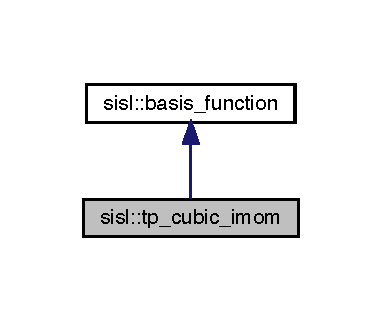
\includegraphics[width=183pt]{classsisl_1_1tp__cubic__imom__inherit__graph}
\end{center}
\end{figure}


Collaboration diagram for sisl\+:\+:tp\+\_\+cubic\+\_\+imom\+:\nopagebreak
\begin{figure}[H]
\begin{center}
\leavevmode
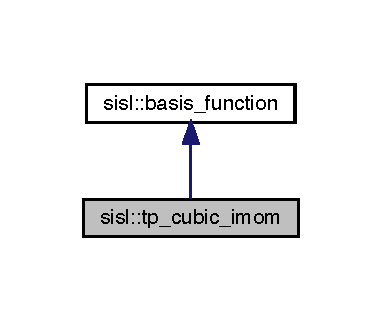
\includegraphics[width=183pt]{classsisl_1_1tp__cubic__imom__coll__graph}
\end{center}
\end{figure}
\subsection*{Static Public Member Functions}
\begin{DoxyCompactItemize}
\item 
\mbox{\Hypertarget{classsisl_1_1tp__cubic__imom_af48f785081da40284238e2f47144db2e}\label{classsisl_1_1tp__cubic__imom_af48f785081da40284238e2f47144db2e}} 
{\footnotesize template$<$int N$>$ }\\static const double {\bfseries phi} (const \hyperlink{namespacesisl_a2069bd5374a9be042ff3ce3306d41e1a}{vector} \&p)
\item 
\mbox{\Hypertarget{classsisl_1_1tp__cubic__imom_aea84d8c194616c55c24755c2c59587ed}\label{classsisl_1_1tp__cubic__imom_aea84d8c194616c55c24755c2c59587ed}} 
{\footnotesize template$<$int N$>$ }\\static const double {\bfseries phi} (const double \&h, const \hyperlink{namespacesisl_a2069bd5374a9be042ff3ce3306d41e1a}{vector} \&p)
\item 
\mbox{\Hypertarget{classsisl_1_1tp__cubic__imom_a52f88d8e9f4e4adf666286c32500c1bb}\label{classsisl_1_1tp__cubic__imom_a52f88d8e9f4e4adf666286c32500c1bb}} 
{\footnotesize template$<$int N$>$ }\\static const double {\bfseries dphi} (const \hyperlink{namespacesisl_a2069bd5374a9be042ff3ce3306d41e1a}{vector} \&p, const int \&d)
\item 
\mbox{\Hypertarget{classsisl_1_1tp__cubic__imom_a9bf0b1172905f6334c92e3823cd64399}\label{classsisl_1_1tp__cubic__imom_a9bf0b1172905f6334c92e3823cd64399}} 
{\footnotesize template$<$int N$>$ }\\static const double {\bfseries dphi} (const double \&h, const \hyperlink{namespacesisl_a2069bd5374a9be042ff3ce3306d41e1a}{vector} \&p, const int \&d)
\item 
\mbox{\Hypertarget{classsisl_1_1tp__cubic__imom_a9a0bbb2100db27a5b8b931338bdfc3b4}\label{classsisl_1_1tp__cubic__imom_a9a0bbb2100db27a5b8b931338bdfc3b4}} 
{\footnotesize template$<$int N$>$ }\\static std\+::vector$<$ \hyperlink{namespacesisl_acd18feee4026583db6185df2b25434aa}{lattice\+\_\+site} $>$ {\bfseries get\+\_\+integer\+\_\+support} ()
\item 
\mbox{\Hypertarget{classsisl_1_1tp__cubic__imom_ad851e32c4fa4af352b831b6c9d1827a8}\label{classsisl_1_1tp__cubic__imom_ad851e32c4fa4af352b831b6c9d1827a8}} 
static bool {\bfseries has\+\_\+derivative} ()
\item 
\mbox{\Hypertarget{classsisl_1_1tp__cubic__imom_ac846d3615a779cc2d2f3201f4bc12c9a}\label{classsisl_1_1tp__cubic__imom_ac846d3615a779cc2d2f3201f4bc12c9a}} 
{\footnotesize template$<$int N, class L , class BF $>$ }\\static double {\bfseries convolution\+\_\+sum} (const \hyperlink{namespacesisl_a2069bd5374a9be042ff3ce3306d41e1a}{vector} \&p, const L $\ast$lattice)
\item 
\mbox{\Hypertarget{classsisl_1_1tp__cubic__imom_af465e487917108dc0a1a4f76118abc36}\label{classsisl_1_1tp__cubic__imom_af465e487917108dc0a1a4f76118abc36}} 
{\footnotesize template$<$int N, class L , class BF $>$ }\\static double {\bfseries convolution\+\_\+sum\+\_\+deriv} (const \hyperlink{namespacesisl_a2069bd5374a9be042ff3ce3306d41e1a}{vector} \&p, const L $\ast$lattice, const int \&component)
\item 
\mbox{\Hypertarget{classsisl_1_1tp__cubic__imom_a958e6a310da8fae4a25b59d443594b3a}\label{classsisl_1_1tp__cubic__imom_a958e6a310da8fae4a25b59d443594b3a}} 
{\footnotesize template$<$int N, class L , class BF $>$ }\\static \hyperlink{namespacesisl_a2069bd5374a9be042ff3ce3306d41e1a}{vector} {\bfseries grad\+\_\+convolution\+\_\+sum} (const \hyperlink{namespacesisl_a2069bd5374a9be042ff3ce3306d41e1a}{vector} \&p, const L $\ast$lattice)
\item 
\mbox{\Hypertarget{classsisl_1_1tp__cubic__imom_a90b70c9920402c1c021b89518318e250}\label{classsisl_1_1tp__cubic__imom_a90b70c9920402c1c021b89518318e250}} 
{\footnotesize template$<$int N, class L , class BF $>$ }\\static \hyperlink{namespacesisl_a2069bd5374a9be042ff3ce3306d41e1a}{vector} {\bfseries grad\+\_\+convolution\+\_\+sum} (const \hyperlink{namespacesisl_a2069bd5374a9be042ff3ce3306d41e1a}{vector} \&p, const L $\ast$base, const L $\ast$$\ast$lattices)
\item 
\mbox{\Hypertarget{classsisl_1_1tp__cubic__imom_a216ad095abfc41041a09154e77f0a763}\label{classsisl_1_1tp__cubic__imom_a216ad095abfc41041a09154e77f0a763}} 
{\footnotesize template$<$int N, class L , class BF $>$ }\\static double {\bfseries convolution\+\_\+sum\+\_\+h} (const \hyperlink{namespacesisl_a2069bd5374a9be042ff3ce3306d41e1a}{vector} \&p, const L $\ast$lattice, const double \&h)
\item 
\mbox{\Hypertarget{classsisl_1_1tp__cubic__imom_a8868ac71fd2df7e1d20c923118d2fe74}\label{classsisl_1_1tp__cubic__imom_a8868ac71fd2df7e1d20c923118d2fe74}} 
{\footnotesize template$<$int N, class L , class BF $>$ }\\static double {\bfseries convolution\+\_\+sum\+\_\+deriv\+\_\+h} (const \hyperlink{namespacesisl_a2069bd5374a9be042ff3ce3306d41e1a}{vector} \&p, const L $\ast$lattice, const int \&component, const double \&h)
\item 
\mbox{\Hypertarget{classsisl_1_1tp__cubic__imom_ab69d77bc980a9d66530a28abb3a6eb3e}\label{classsisl_1_1tp__cubic__imom_ab69d77bc980a9d66530a28abb3a6eb3e}} 
{\footnotesize template$<$int N, class L , class BF $>$ }\\static \hyperlink{namespacesisl_a2069bd5374a9be042ff3ce3306d41e1a}{vector} {\bfseries grad\+\_\+convolution\+\_\+sum\+\_\+h} (const \hyperlink{namespacesisl_a2069bd5374a9be042ff3ce3306d41e1a}{vector} \&p, const L $\ast$lattice, const double \&h)
\item 
\mbox{\Hypertarget{classsisl_1_1tp__cubic__imom_ad04f216c381d5dfce904a063a1328011}\label{classsisl_1_1tp__cubic__imom_ad04f216c381d5dfce904a063a1328011}} 
{\footnotesize template$<$int N, class L , class BF $>$ }\\static \hyperlink{namespacesisl_a2069bd5374a9be042ff3ce3306d41e1a}{vector} {\bfseries grad\+\_\+convolution\+\_\+sum\+\_\+h} (const \hyperlink{namespacesisl_a2069bd5374a9be042ff3ce3306d41e1a}{vector} \&p, const L $\ast$base, const L $\ast$$\ast$lattices, const double \&h)
\end{DoxyCompactItemize}


\subsection{Detailed Description}
Tensor product cubic interpolating M\+OM. 



The documentation for this class was generated from the following file\+:\begin{DoxyCompactItemize}
\item 
/\+Users/joshuahoracsek/\+Projects/sisl\+\_\+redux/include/sisl/basis/tp\+\_\+cubic\+\_\+imom.\+hpp\end{DoxyCompactItemize}

\hypertarget{classsisl_1_1tp__linear}{}\section{sisl\+:\+:tp\+\_\+linear Class Reference}
\label{classsisl_1_1tp__linear}\index{sisl\+::tp\+\_\+linear@{sisl\+::tp\+\_\+linear}}


Tensor product linear basis function. Tensor product linear basis function. On the planar and cubic Cartesian lattices, we have F\+A\+S\+T\+\_\+\+B\+A\+S\+ES which correspond to bilinear and trilinear interpolation.  




{\ttfamily \#include $<$tp\+\_\+linear.\+hpp$>$}



Inheritance diagram for sisl\+:\+:tp\+\_\+linear\+:\nopagebreak
\begin{figure}[H]
\begin{center}
\leavevmode
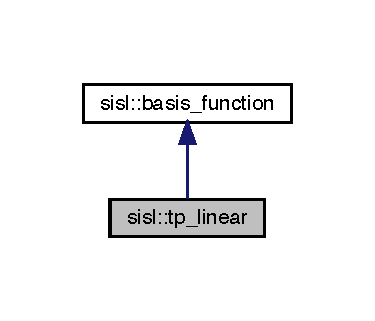
\includegraphics[width=180pt]{classsisl_1_1tp__linear__inherit__graph}
\end{center}
\end{figure}


Collaboration diagram for sisl\+:\+:tp\+\_\+linear\+:\nopagebreak
\begin{figure}[H]
\begin{center}
\leavevmode
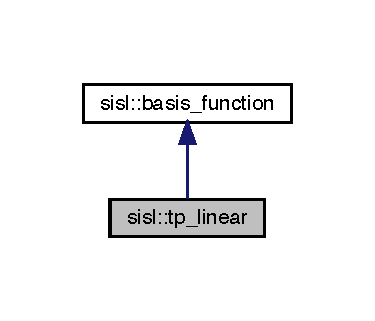
\includegraphics[width=180pt]{classsisl_1_1tp__linear__coll__graph}
\end{center}
\end{figure}
\subsection*{Static Public Member Functions}
\begin{DoxyCompactItemize}
\item 
\mbox{\Hypertarget{classsisl_1_1tp__linear_a896ed9c644c3c7318e6519e9b44b5df1}\label{classsisl_1_1tp__linear_a896ed9c644c3c7318e6519e9b44b5df1}} 
{\footnotesize template$<$int N$>$ }\\static const double {\bfseries phi} (const \hyperlink{namespacesisl_a2069bd5374a9be042ff3ce3306d41e1a}{vector} \&p)
\item 
\mbox{\Hypertarget{classsisl_1_1tp__linear_a48d52465e7b1ef3956f1d7409dfa7f01}\label{classsisl_1_1tp__linear_a48d52465e7b1ef3956f1d7409dfa7f01}} 
{\footnotesize template$<$int N$>$ }\\static const double {\bfseries phi} (const double \&h, const \hyperlink{namespacesisl_a2069bd5374a9be042ff3ce3306d41e1a}{vector} \&p)
\item 
\mbox{\Hypertarget{classsisl_1_1tp__linear_a608311c529198387c06276c38b53de24}\label{classsisl_1_1tp__linear_a608311c529198387c06276c38b53de24}} 
{\footnotesize template$<$int N$>$ }\\static const double {\bfseries dphi} (const \hyperlink{namespacesisl_a2069bd5374a9be042ff3ce3306d41e1a}{vector} \&p, const int \&d)
\item 
\mbox{\Hypertarget{classsisl_1_1tp__linear_a9d749bb2fe2f8bc75a1c93ed61ef742e}\label{classsisl_1_1tp__linear_a9d749bb2fe2f8bc75a1c93ed61ef742e}} 
{\footnotesize template$<$int N$>$ }\\static const double {\bfseries dphi} (const double \&h, const \hyperlink{namespacesisl_a2069bd5374a9be042ff3ce3306d41e1a}{vector} \&p, const int \&d)
\item 
\mbox{\Hypertarget{classsisl_1_1tp__linear_addadc6697a7c631f1b5a25082f73db1e}\label{classsisl_1_1tp__linear_addadc6697a7c631f1b5a25082f73db1e}} 
{\footnotesize template$<$int N$>$ }\\static std\+::vector$<$ \hyperlink{namespacesisl_acd18feee4026583db6185df2b25434aa}{lattice\+\_\+site} $>$ {\bfseries get\+\_\+integer\+\_\+support} ()
\item 
\mbox{\Hypertarget{classsisl_1_1tp__linear_a152b711e8947e3b44cc5236a0bd1b195}\label{classsisl_1_1tp__linear_a152b711e8947e3b44cc5236a0bd1b195}} 
static bool {\bfseries has\+\_\+derivative} ()
\item 
\mbox{\Hypertarget{classsisl_1_1tp__linear_ac0f1255414dfe1b16376428cae47d407}\label{classsisl_1_1tp__linear_ac0f1255414dfe1b16376428cae47d407}} 
{\footnotesize template$<$int N, class L , class BF $>$ }\\static double {\bfseries convolution\+\_\+sum} (const \hyperlink{namespacesisl_a2069bd5374a9be042ff3ce3306d41e1a}{vector} \&p, const L $\ast$lattice)
\item 
\mbox{\Hypertarget{classsisl_1_1tp__linear_adee0c9f2ee87504cc2ef376b2e2c359a}\label{classsisl_1_1tp__linear_adee0c9f2ee87504cc2ef376b2e2c359a}} 
{\footnotesize template$<$int N, class L , class BF $>$ }\\static double {\bfseries convolution\+\_\+sum\+\_\+deriv} (const \hyperlink{namespacesisl_a2069bd5374a9be042ff3ce3306d41e1a}{vector} \&p, const L $\ast$lattice, const int \&component)
\item 
\mbox{\Hypertarget{classsisl_1_1tp__linear_a98a633bfd39ce17e449820bfbff12cac}\label{classsisl_1_1tp__linear_a98a633bfd39ce17e449820bfbff12cac}} 
{\footnotesize template$<$int N, class L , class BF $>$ }\\static \hyperlink{namespacesisl_a2069bd5374a9be042ff3ce3306d41e1a}{vector} {\bfseries grad\+\_\+convolution\+\_\+sum} (const \hyperlink{namespacesisl_a2069bd5374a9be042ff3ce3306d41e1a}{vector} \&p, const L $\ast$lattice)
\item 
\mbox{\Hypertarget{classsisl_1_1tp__linear_a101bc6459e8046815c7f5ec093e983f8}\label{classsisl_1_1tp__linear_a101bc6459e8046815c7f5ec093e983f8}} 
{\footnotesize template$<$int N, class L , class BF $>$ }\\static \hyperlink{namespacesisl_a2069bd5374a9be042ff3ce3306d41e1a}{vector} {\bfseries grad\+\_\+convolution\+\_\+sum} (const \hyperlink{namespacesisl_a2069bd5374a9be042ff3ce3306d41e1a}{vector} \&p, const L $\ast$base, const L $\ast$$\ast$lattices)
\item 
\mbox{\Hypertarget{classsisl_1_1tp__linear_a01ac307fbb6d596d0397a10759540076}\label{classsisl_1_1tp__linear_a01ac307fbb6d596d0397a10759540076}} 
{\footnotesize template$<$int N, class L , class BF $>$ }\\static double {\bfseries convolution\+\_\+sum\+\_\+h} (const \hyperlink{namespacesisl_a2069bd5374a9be042ff3ce3306d41e1a}{vector} \&p, const L $\ast$lattice, const double \&h)
\item 
\mbox{\Hypertarget{classsisl_1_1tp__linear_a18c6496aaa2e3fbfe523f0251cd73da9}\label{classsisl_1_1tp__linear_a18c6496aaa2e3fbfe523f0251cd73da9}} 
{\footnotesize template$<$int N, class L , class BF $>$ }\\static double {\bfseries convolution\+\_\+sum\+\_\+deriv\+\_\+h} (const \hyperlink{namespacesisl_a2069bd5374a9be042ff3ce3306d41e1a}{vector} \&p, const L $\ast$lattice, const int \&component, const double \&h)
\item 
\mbox{\Hypertarget{classsisl_1_1tp__linear_ab28a77f856fa7f0e35f3f6d49daadeb5}\label{classsisl_1_1tp__linear_ab28a77f856fa7f0e35f3f6d49daadeb5}} 
{\footnotesize template$<$int N, class L , class BF $>$ }\\static \hyperlink{namespacesisl_a2069bd5374a9be042ff3ce3306d41e1a}{vector} {\bfseries grad\+\_\+convolution\+\_\+sum\+\_\+h} (const \hyperlink{namespacesisl_a2069bd5374a9be042ff3ce3306d41e1a}{vector} \&p, const L $\ast$lattice, const double \&h)
\item 
\mbox{\Hypertarget{classsisl_1_1tp__linear_a81674ecd19a9729519bb7003c510de81}\label{classsisl_1_1tp__linear_a81674ecd19a9729519bb7003c510de81}} 
{\footnotesize template$<$int N, class L , class BF $>$ }\\static \hyperlink{namespacesisl_a2069bd5374a9be042ff3ce3306d41e1a}{vector} {\bfseries grad\+\_\+convolution\+\_\+sum\+\_\+h} (const \hyperlink{namespacesisl_a2069bd5374a9be042ff3ce3306d41e1a}{vector} \&p, const L $\ast$base, const L $\ast$$\ast$lattices, const double \&h)
\end{DoxyCompactItemize}


\subsection{Detailed Description}
Tensor product linear basis function. Tensor product linear basis function. On the planar and cubic Cartesian lattices, we have F\+A\+S\+T\+\_\+\+B\+A\+S\+ES which correspond to bilinear and trilinear interpolation. 

The documentation for this class was generated from the following file\+:\begin{DoxyCompactItemize}
\item 
/\+Users/joshuahoracsek/\+Projects/sisl\+\_\+redux/include/sisl/basis/tp\+\_\+linear.\+hpp\end{DoxyCompactItemize}

\hypertarget{classsisl_1_1tp__quadratic}{}\section{sisl\+:\+:tp\+\_\+quadratic Class Reference}
\label{classsisl_1_1tp__quadratic}\index{sisl\+::tp\+\_\+quadratic@{sisl\+::tp\+\_\+quadratic}}


Tensor product quadratic spline.  




{\ttfamily \#include $<$tp\+\_\+quadratic.\+hpp$>$}



Inheritance diagram for sisl\+:\+:tp\+\_\+quadratic\+:\nopagebreak
\begin{figure}[H]
\begin{center}
\leavevmode
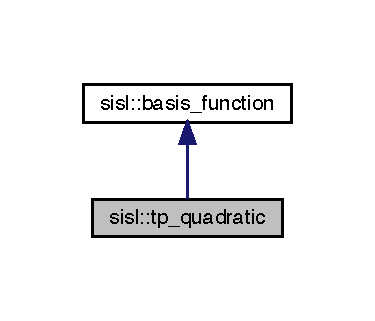
\includegraphics[width=180pt]{classsisl_1_1tp__quadratic__inherit__graph}
\end{center}
\end{figure}


Collaboration diagram for sisl\+:\+:tp\+\_\+quadratic\+:\nopagebreak
\begin{figure}[H]
\begin{center}
\leavevmode
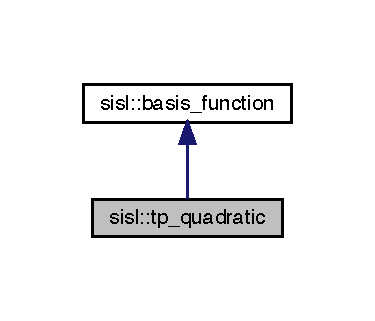
\includegraphics[width=180pt]{classsisl_1_1tp__quadratic__coll__graph}
\end{center}
\end{figure}
\subsection*{Static Public Member Functions}
\begin{DoxyCompactItemize}
\item 
\mbox{\Hypertarget{classsisl_1_1tp__quadratic_ab296bef374fc6cefe2ec7d80689b448e}\label{classsisl_1_1tp__quadratic_ab296bef374fc6cefe2ec7d80689b448e}} 
{\footnotesize template$<$int N$>$ }\\static const double {\bfseries phi} (const \hyperlink{namespacesisl_a2069bd5374a9be042ff3ce3306d41e1a}{vector} \&p)
\item 
\mbox{\Hypertarget{classsisl_1_1tp__quadratic_a6da6a6fbeae8cf3f51bd8eac943abb50}\label{classsisl_1_1tp__quadratic_a6da6a6fbeae8cf3f51bd8eac943abb50}} 
{\footnotesize template$<$int N$>$ }\\static const double {\bfseries phi} (const double \&h, const \hyperlink{namespacesisl_a2069bd5374a9be042ff3ce3306d41e1a}{vector} \&p)
\item 
\mbox{\Hypertarget{classsisl_1_1tp__quadratic_a1958f4481128150832c89c56ed20b98c}\label{classsisl_1_1tp__quadratic_a1958f4481128150832c89c56ed20b98c}} 
{\footnotesize template$<$int N$>$ }\\static const double {\bfseries dphi} (const \hyperlink{namespacesisl_a2069bd5374a9be042ff3ce3306d41e1a}{vector} \&p, const int \&d)
\item 
\mbox{\Hypertarget{classsisl_1_1tp__quadratic_a3a2e1e155c83f696ff4216877c9bb018}\label{classsisl_1_1tp__quadratic_a3a2e1e155c83f696ff4216877c9bb018}} 
{\footnotesize template$<$int N$>$ }\\static const double {\bfseries dphi} (const double \&h, const \hyperlink{namespacesisl_a2069bd5374a9be042ff3ce3306d41e1a}{vector} \&p, const int \&d)
\item 
\mbox{\Hypertarget{classsisl_1_1tp__quadratic_aa463fc4a5127a7dfebe15d4f06182fce}\label{classsisl_1_1tp__quadratic_aa463fc4a5127a7dfebe15d4f06182fce}} 
{\footnotesize template$<$int N$>$ }\\static std\+::vector$<$ \hyperlink{namespacesisl_acd18feee4026583db6185df2b25434aa}{lattice\+\_\+site} $>$ {\bfseries get\+\_\+integer\+\_\+support} ()
\item 
\mbox{\Hypertarget{classsisl_1_1tp__quadratic_abe066745c28ae8424c0fb80b524c3b39}\label{classsisl_1_1tp__quadratic_abe066745c28ae8424c0fb80b524c3b39}} 
static bool {\bfseries has\+\_\+derivative} ()
\item 
\mbox{\Hypertarget{classsisl_1_1tp__quadratic_a850082ac2adb0124b7994c18af6dcc53}\label{classsisl_1_1tp__quadratic_a850082ac2adb0124b7994c18af6dcc53}} 
{\footnotesize template$<$int N, class L , class BF $>$ }\\static double {\bfseries convolution\+\_\+sum} (const \hyperlink{namespacesisl_a2069bd5374a9be042ff3ce3306d41e1a}{vector} \&p, const L $\ast$lattice)
\item 
\mbox{\Hypertarget{classsisl_1_1tp__quadratic_a7280d1af6563968684553ee3b99dd0f1}\label{classsisl_1_1tp__quadratic_a7280d1af6563968684553ee3b99dd0f1}} 
{\footnotesize template$<$int N, class L , class BF $>$ }\\static double {\bfseries convolution\+\_\+sum\+\_\+deriv} (const \hyperlink{namespacesisl_a2069bd5374a9be042ff3ce3306d41e1a}{vector} \&p, const L $\ast$lattice, const int \&component)
\item 
\mbox{\Hypertarget{classsisl_1_1tp__quadratic_a2243705ea86692e64149d82e88a0e0fc}\label{classsisl_1_1tp__quadratic_a2243705ea86692e64149d82e88a0e0fc}} 
{\footnotesize template$<$int N, class L , class BF $>$ }\\static \hyperlink{namespacesisl_a2069bd5374a9be042ff3ce3306d41e1a}{vector} {\bfseries grad\+\_\+convolution\+\_\+sum} (const \hyperlink{namespacesisl_a2069bd5374a9be042ff3ce3306d41e1a}{vector} \&p, const L $\ast$lattice)
\item 
\mbox{\Hypertarget{classsisl_1_1tp__quadratic_afe95f0af6e952f68ca431ef619824829}\label{classsisl_1_1tp__quadratic_afe95f0af6e952f68ca431ef619824829}} 
{\footnotesize template$<$int N, class L , class BF $>$ }\\static \hyperlink{namespacesisl_a2069bd5374a9be042ff3ce3306d41e1a}{vector} {\bfseries grad\+\_\+convolution\+\_\+sum} (const \hyperlink{namespacesisl_a2069bd5374a9be042ff3ce3306d41e1a}{vector} \&p, const L $\ast$base, const L $\ast$$\ast$lattices)
\item 
\mbox{\Hypertarget{classsisl_1_1tp__quadratic_a86821dd0fec5985b5d24a753168f3db7}\label{classsisl_1_1tp__quadratic_a86821dd0fec5985b5d24a753168f3db7}} 
{\footnotesize template$<$int N, class L , class BF $>$ }\\static double {\bfseries convolution\+\_\+sum\+\_\+h} (const \hyperlink{namespacesisl_a2069bd5374a9be042ff3ce3306d41e1a}{vector} \&p, const L $\ast$lattice, const double \&h)
\item 
\mbox{\Hypertarget{classsisl_1_1tp__quadratic_a6e136b55112a47e19693c20b0c8d685f}\label{classsisl_1_1tp__quadratic_a6e136b55112a47e19693c20b0c8d685f}} 
{\footnotesize template$<$int N, class L , class BF $>$ }\\static double {\bfseries convolution\+\_\+sum\+\_\+deriv\+\_\+h} (const \hyperlink{namespacesisl_a2069bd5374a9be042ff3ce3306d41e1a}{vector} \&p, const L $\ast$lattice, const int \&component, const double \&h)
\item 
\mbox{\Hypertarget{classsisl_1_1tp__quadratic_a04f7d2e073ef040804cc80a97798e18e}\label{classsisl_1_1tp__quadratic_a04f7d2e073ef040804cc80a97798e18e}} 
{\footnotesize template$<$int N, class L , class BF $>$ }\\static \hyperlink{namespacesisl_a2069bd5374a9be042ff3ce3306d41e1a}{vector} {\bfseries grad\+\_\+convolution\+\_\+sum\+\_\+h} (const \hyperlink{namespacesisl_a2069bd5374a9be042ff3ce3306d41e1a}{vector} \&p, const L $\ast$lattice, const double \&h)
\item 
\mbox{\Hypertarget{classsisl_1_1tp__quadratic_a20a5e68fe8020f5ce933a7ebc236bf5e}\label{classsisl_1_1tp__quadratic_a20a5e68fe8020f5ce933a7ebc236bf5e}} 
{\footnotesize template$<$int N, class L , class BF $>$ }\\static \hyperlink{namespacesisl_a2069bd5374a9be042ff3ce3306d41e1a}{vector} {\bfseries grad\+\_\+convolution\+\_\+sum\+\_\+h} (const \hyperlink{namespacesisl_a2069bd5374a9be042ff3ce3306d41e1a}{vector} \&p, const L $\ast$base, const L $\ast$$\ast$lattices, const double \&h)
\end{DoxyCompactItemize}


\subsection{Detailed Description}
Tensor product quadratic spline. 



The documentation for this class was generated from the following file\+:\begin{DoxyCompactItemize}
\item 
/\+Users/joshuahoracsek/\+Projects/sisl\+\_\+redux/include/sisl/basis/tp\+\_\+quadratic.\+hpp\end{DoxyCompactItemize}

\hypertarget{structsisl_1_1triangle}{}\section{sisl\+:\+:triangle Struct Reference}
\label{structsisl_1_1triangle}\index{sisl\+::triangle@{sisl\+::triangle}}


Triangle in 3D space.  




{\ttfamily \#include $<$primitives.\+hpp$>$}



Collaboration diagram for sisl\+:\+:triangle\+:\nopagebreak
\begin{figure}[H]
\begin{center}
\leavevmode
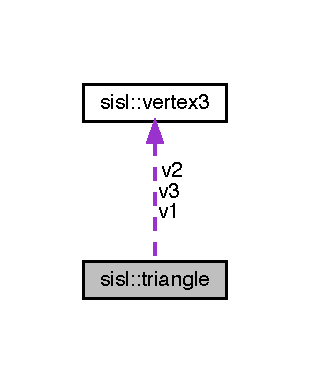
\includegraphics[width=149pt]{structsisl_1_1triangle__coll__graph}
\end{center}
\end{figure}
\subsection*{Public Member Functions}
\begin{DoxyCompactItemize}
\item 
\hyperlink{structsisl_1_1triangle_a0e0dcd17f1c5e16ecb79daceb604c19a}{triangle} (const \hyperlink{structsisl_1_1vertex3}{vertex3} \&\+\_\+v1, const \hyperlink{structsisl_1_1vertex3}{vertex3} \&\+\_\+v2, const \hyperlink{structsisl_1_1vertex3}{vertex3} \&\+\_\+v3)
\item 
\hyperlink{structsisl_1_1triangle_adae1a504fbc6782f22a434897ad39b1c}{triangle} (const \hyperlink{structsisl_1_1triangle}{triangle} \&\+\_\+t)
\end{DoxyCompactItemize}
\subsection*{Public Attributes}
\begin{DoxyCompactItemize}
\item 
\mbox{\Hypertarget{structsisl_1_1triangle_ad86734de300b5c09c56d5aba5ecf33f7}\label{structsisl_1_1triangle_ad86734de300b5c09c56d5aba5ecf33f7}} 
\hyperlink{structsisl_1_1vertex3}{vertex3} \hyperlink{structsisl_1_1triangle_ad86734de300b5c09c56d5aba5ecf33f7}{v1}
\begin{DoxyCompactList}\small\item\em triangle vertex 1 \end{DoxyCompactList}\item 
\mbox{\Hypertarget{structsisl_1_1triangle_a6f6ca60258efc6eed6f8fe52d0945c7e}\label{structsisl_1_1triangle_a6f6ca60258efc6eed6f8fe52d0945c7e}} 
\hyperlink{structsisl_1_1vertex3}{vertex3} \hyperlink{structsisl_1_1triangle_a6f6ca60258efc6eed6f8fe52d0945c7e}{v2}
\begin{DoxyCompactList}\small\item\em triangle vertex 2 \end{DoxyCompactList}\item 
\mbox{\Hypertarget{structsisl_1_1triangle_a5e1cdf5601cccbaaa1ff340003f9c54d}\label{structsisl_1_1triangle_a5e1cdf5601cccbaaa1ff340003f9c54d}} 
\hyperlink{structsisl_1_1vertex3}{vertex3} \hyperlink{structsisl_1_1triangle_a5e1cdf5601cccbaaa1ff340003f9c54d}{v3}
\begin{DoxyCompactList}\small\item\em triangle vertex 3 \end{DoxyCompactList}\end{DoxyCompactItemize}


\subsection{Detailed Description}
Triangle in 3D space. 

A collection of three points that creates a ploygon in space 

\subsection{Constructor \& Destructor Documentation}
\mbox{\Hypertarget{structsisl_1_1triangle_a0e0dcd17f1c5e16ecb79daceb604c19a}\label{structsisl_1_1triangle_a0e0dcd17f1c5e16ecb79daceb604c19a}} 
\index{sisl\+::triangle@{sisl\+::triangle}!triangle@{triangle}}
\index{triangle@{triangle}!sisl\+::triangle@{sisl\+::triangle}}
\subsubsection{\texorpdfstring{triangle()}{triangle()}\hspace{0.1cm}{\footnotesize\ttfamily [1/2]}}
{\footnotesize\ttfamily sisl\+::triangle\+::triangle (\begin{DoxyParamCaption}\item[{const \hyperlink{structsisl_1_1vertex3}{vertex3} \&}]{\+\_\+v1,  }\item[{const \hyperlink{structsisl_1_1vertex3}{vertex3} \&}]{\+\_\+v2,  }\item[{const \hyperlink{structsisl_1_1vertex3}{vertex3} \&}]{\+\_\+v3 }\end{DoxyParamCaption})\hspace{0.3cm}{\ttfamily [inline]}}

Ray constructor 
\begin{DoxyParams}{Parameters}
{\em \+\_\+v1,\+\_\+v2,\+\_\+v3} & The vertices that make up a triangle. \\
\hline
\end{DoxyParams}
\mbox{\Hypertarget{structsisl_1_1triangle_adae1a504fbc6782f22a434897ad39b1c}\label{structsisl_1_1triangle_adae1a504fbc6782f22a434897ad39b1c}} 
\index{sisl\+::triangle@{sisl\+::triangle}!triangle@{triangle}}
\index{triangle@{triangle}!sisl\+::triangle@{sisl\+::triangle}}
\subsubsection{\texorpdfstring{triangle()}{triangle()}\hspace{0.1cm}{\footnotesize\ttfamily [2/2]}}
{\footnotesize\ttfamily sisl\+::triangle\+::triangle (\begin{DoxyParamCaption}\item[{const \hyperlink{structsisl_1_1triangle}{triangle} \&}]{\+\_\+t }\end{DoxyParamCaption})\hspace{0.3cm}{\ttfamily [inline]}}

Plane copy constructor 
\begin{DoxyParams}{Parameters}
{\em \+\_\+p} & A plane to copy \\
\hline
\end{DoxyParams}


The documentation for this struct was generated from the following file\+:\begin{DoxyCompactItemize}
\item 
/\+Users/joshuahoracsek/\+Projects/sisl\+\_\+redux/include/sisl/primitives.\+hpp\end{DoxyCompactItemize}

\hypertarget{structsisl_1_1vertex3}{}\section{sisl\+:\+:vertex3 Struct Reference}
\label{structsisl_1_1vertex3}\index{sisl\+::vertex3@{sisl\+::vertex3}}


3D vertex.  




{\ttfamily \#include $<$primitives.\+hpp$>$}

\subsection*{Public Member Functions}
\begin{DoxyCompactItemize}
\item 
\hyperlink{structsisl_1_1vertex3_ab40c72beb889e4cca21d372eff7886ef}{vertex3} (const \hyperlink{namespacesisl_a2069bd5374a9be042ff3ce3306d41e1a}{vector} \&\+\_\+p, const \hyperlink{namespacesisl_a2069bd5374a9be042ff3ce3306d41e1a}{vector} \&\+\_\+n)
\item 
\hyperlink{structsisl_1_1vertex3_a9ced36fc7fbadbb1a9fd285529417f28}{vertex3} (const double \&x, const double \&y, const double \&z, const double \&i, const double \&j, const double \&k)
\item 
\hyperlink{structsisl_1_1vertex3_a689f16f717542968ed5ba74129866228}{vertex3} (const \hyperlink{structsisl_1_1vertex3}{vertex3} \&\+\_\+v)
\end{DoxyCompactItemize}
\subsection*{Public Attributes}
\begin{DoxyCompactItemize}
\item 
\mbox{\Hypertarget{structsisl_1_1vertex3_aa67a470e2653f995cc2f20da7551e80a}\label{structsisl_1_1vertex3_aa67a470e2653f995cc2f20da7551e80a}} 
\hyperlink{namespacesisl_a2069bd5374a9be042ff3ce3306d41e1a}{vector} \hyperlink{structsisl_1_1vertex3_aa67a470e2653f995cc2f20da7551e80a}{p}
\begin{DoxyCompactList}\small\item\em vertex spatial location \end{DoxyCompactList}\item 
\mbox{\Hypertarget{structsisl_1_1vertex3_a04353827513fa8173bf690d77004a143}\label{structsisl_1_1vertex3_a04353827513fa8173bf690d77004a143}} 
\hyperlink{namespacesisl_a2069bd5374a9be042ff3ce3306d41e1a}{vector} \hyperlink{structsisl_1_1vertex3_a04353827513fa8173bf690d77004a143}{n}
\begin{DoxyCompactList}\small\item\em vertex normal direction \end{DoxyCompactList}\end{DoxyCompactItemize}


\subsection{Detailed Description}
3D vertex. 

A vertex in the graphics sense, i.\+e. a spatial point, and a normal to help shading heuristics. 

\subsection{Constructor \& Destructor Documentation}
\mbox{\Hypertarget{structsisl_1_1vertex3_ab40c72beb889e4cca21d372eff7886ef}\label{structsisl_1_1vertex3_ab40c72beb889e4cca21d372eff7886ef}} 
\index{sisl\+::vertex3@{sisl\+::vertex3}!vertex3@{vertex3}}
\index{vertex3@{vertex3}!sisl\+::vertex3@{sisl\+::vertex3}}
\subsubsection{\texorpdfstring{vertex3()}{vertex3()}\hspace{0.1cm}{\footnotesize\ttfamily [1/3]}}
{\footnotesize\ttfamily sisl\+::vertex3\+::vertex3 (\begin{DoxyParamCaption}\item[{const \hyperlink{namespacesisl_a2069bd5374a9be042ff3ce3306d41e1a}{vector} \&}]{\+\_\+p,  }\item[{const \hyperlink{namespacesisl_a2069bd5374a9be042ff3ce3306d41e1a}{vector} \&}]{\+\_\+n }\end{DoxyParamCaption})\hspace{0.3cm}{\ttfamily [inline]}}

Vertex constructor 
\begin{DoxyParams}{Parameters}
{\em \+\_\+p} & Spatial location of a point. \\
\hline
{\em \+\_\+n} & Point normal. \\
\hline
\end{DoxyParams}
\mbox{\Hypertarget{structsisl_1_1vertex3_a9ced36fc7fbadbb1a9fd285529417f28}\label{structsisl_1_1vertex3_a9ced36fc7fbadbb1a9fd285529417f28}} 
\index{sisl\+::vertex3@{sisl\+::vertex3}!vertex3@{vertex3}}
\index{vertex3@{vertex3}!sisl\+::vertex3@{sisl\+::vertex3}}
\subsubsection{\texorpdfstring{vertex3()}{vertex3()}\hspace{0.1cm}{\footnotesize\ttfamily [2/3]}}
{\footnotesize\ttfamily sisl\+::vertex3\+::vertex3 (\begin{DoxyParamCaption}\item[{const double \&}]{x,  }\item[{const double \&}]{y,  }\item[{const double \&}]{z,  }\item[{const double \&}]{i,  }\item[{const double \&}]{j,  }\item[{const double \&}]{k }\end{DoxyParamCaption})\hspace{0.3cm}{\ttfamily [inline]}}

Vertex constructor 
\begin{DoxyParams}{Parameters}
{\em x,y,z} & Spatial location of a point. \\
\hline
{\em i,j,k} & Point normal. \\
\hline
\end{DoxyParams}
\mbox{\Hypertarget{structsisl_1_1vertex3_a689f16f717542968ed5ba74129866228}\label{structsisl_1_1vertex3_a689f16f717542968ed5ba74129866228}} 
\index{sisl\+::vertex3@{sisl\+::vertex3}!vertex3@{vertex3}}
\index{vertex3@{vertex3}!sisl\+::vertex3@{sisl\+::vertex3}}
\subsubsection{\texorpdfstring{vertex3()}{vertex3()}\hspace{0.1cm}{\footnotesize\ttfamily [3/3]}}
{\footnotesize\ttfamily sisl\+::vertex3\+::vertex3 (\begin{DoxyParamCaption}\item[{const \hyperlink{structsisl_1_1vertex3}{vertex3} \&}]{\+\_\+v }\end{DoxyParamCaption})\hspace{0.3cm}{\ttfamily [inline]}}

Vertex copy constructor 
\begin{DoxyParams}{Parameters}
{\em \+\_\+v} & A vertex to copy \\
\hline
\end{DoxyParams}


The documentation for this struct was generated from the following file\+:\begin{DoxyCompactItemize}
\item 
/\+Users/joshuahoracsek/\+Projects/sisl\+\_\+redux/include/sisl/primitives.\+hpp\end{DoxyCompactItemize}

\hypertarget{classsisl_1_1zp3__element}{}\section{sisl\+:\+:zp3\+\_\+element Class Reference}
\label{classsisl_1_1zp3__element}\index{sisl\+::zp3\+\_\+element@{sisl\+::zp3\+\_\+element}}


Inheritance diagram for sisl\+:\+:zp3\+\_\+element\+:\nopagebreak
\begin{figure}[H]
\begin{center}
\leavevmode
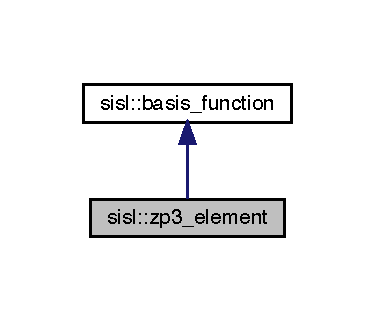
\includegraphics[width=180pt]{classsisl_1_1zp3__element__inherit__graph}
\end{center}
\end{figure}


Collaboration diagram for sisl\+:\+:zp3\+\_\+element\+:\nopagebreak
\begin{figure}[H]
\begin{center}
\leavevmode
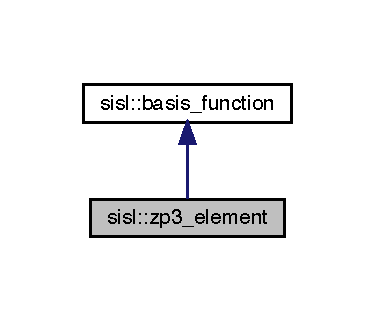
\includegraphics[width=180pt]{classsisl_1_1zp3__element__coll__graph}
\end{center}
\end{figure}
\subsection*{Static Public Member Functions}
\begin{DoxyCompactItemize}
\item 
\mbox{\Hypertarget{classsisl_1_1zp3__element_a99fd4709ef8de0d88dd34fd60a9f0416}\label{classsisl_1_1zp3__element_a99fd4709ef8de0d88dd34fd60a9f0416}} 
{\footnotesize template$<$int N$>$ }\\static const double {\bfseries phi} (const \hyperlink{namespacesisl_a2069bd5374a9be042ff3ce3306d41e1a}{vector} \&p)
\item 
\mbox{\Hypertarget{classsisl_1_1zp3__element_ac26a648ab1147bd5ca1ee7e99ab20807}\label{classsisl_1_1zp3__element_ac26a648ab1147bd5ca1ee7e99ab20807}} 
{\footnotesize template$<$int N$>$ }\\static const double {\bfseries phi} (const double \&h, const \hyperlink{namespacesisl_a2069bd5374a9be042ff3ce3306d41e1a}{vector} \&p)
\item 
\mbox{\Hypertarget{classsisl_1_1zp3__element_a6a1d18a8deb3bfc5bede41c552d577de}\label{classsisl_1_1zp3__element_a6a1d18a8deb3bfc5bede41c552d577de}} 
{\footnotesize template$<$int N$>$ }\\static const double {\bfseries dphi} (const \hyperlink{namespacesisl_a2069bd5374a9be042ff3ce3306d41e1a}{vector} \&p, const int \&d)
\item 
\mbox{\Hypertarget{classsisl_1_1zp3__element_a5c28b9e7412e474a6c5f05a8b69c483d}\label{classsisl_1_1zp3__element_a5c28b9e7412e474a6c5f05a8b69c483d}} 
{\footnotesize template$<$int N$>$ }\\static const double {\bfseries dphi} (const double \&h, const \hyperlink{namespacesisl_a2069bd5374a9be042ff3ce3306d41e1a}{vector} \&p, const int \&d)
\item 
\mbox{\Hypertarget{classsisl_1_1zp3__element_ad07351efdd0fe9a39a45397afeceba63}\label{classsisl_1_1zp3__element_ad07351efdd0fe9a39a45397afeceba63}} 
{\footnotesize template$<$int N$>$ }\\static std\+::vector$<$ \hyperlink{namespacesisl_acd18feee4026583db6185df2b25434aa}{lattice\+\_\+site} $>$ {\bfseries get\+\_\+integer\+\_\+support} ()
\item 
\mbox{\Hypertarget{classsisl_1_1zp3__element_adba6602f5ff3802d5452c1bc1cc34986}\label{classsisl_1_1zp3__element_adba6602f5ff3802d5452c1bc1cc34986}} 
{\footnotesize template$<$int N, class L , class BF $>$ }\\static double {\bfseries convolution\+\_\+sum} (const \hyperlink{namespacesisl_a2069bd5374a9be042ff3ce3306d41e1a}{vector} \&p, const L $\ast$lattice)
\item 
\mbox{\Hypertarget{classsisl_1_1zp3__element_ad7aa5ca329acb51e1b5f0416e2ef66f4}\label{classsisl_1_1zp3__element_ad7aa5ca329acb51e1b5f0416e2ef66f4}} 
{\footnotesize template$<$int N, class L , class BF $>$ }\\static double {\bfseries convolution\+\_\+sum\+\_\+deriv} (const \hyperlink{namespacesisl_a2069bd5374a9be042ff3ce3306d41e1a}{vector} \&p, const L $\ast$lattice, const int \&component)
\item 
\mbox{\Hypertarget{classsisl_1_1zp3__element_ab58ef07abf797c578a37d3dfc9fa3273}\label{classsisl_1_1zp3__element_ab58ef07abf797c578a37d3dfc9fa3273}} 
{\footnotesize template$<$int N, class L , class BF $>$ }\\static \hyperlink{namespacesisl_a2069bd5374a9be042ff3ce3306d41e1a}{vector} {\bfseries grad\+\_\+convolution\+\_\+sum} (const \hyperlink{namespacesisl_a2069bd5374a9be042ff3ce3306d41e1a}{vector} \&p, const L $\ast$lattice)
\item 
\mbox{\Hypertarget{classsisl_1_1zp3__element_aa6703690d865d70809a46ea06e296ae7}\label{classsisl_1_1zp3__element_aa6703690d865d70809a46ea06e296ae7}} 
{\footnotesize template$<$int N, class L , class BF $>$ }\\static \hyperlink{namespacesisl_a2069bd5374a9be042ff3ce3306d41e1a}{vector} {\bfseries grad\+\_\+convolution\+\_\+sum} (const \hyperlink{namespacesisl_a2069bd5374a9be042ff3ce3306d41e1a}{vector} \&p, const L $\ast$base, const L $\ast$$\ast$lattices)
\item 
\mbox{\Hypertarget{classsisl_1_1zp3__element_a35e259e74d2b0592eca4daff2bc4b34d}\label{classsisl_1_1zp3__element_a35e259e74d2b0592eca4daff2bc4b34d}} 
{\footnotesize template$<$int N, class L , class BF $>$ }\\static double {\bfseries convolution\+\_\+sum\+\_\+h} (const \hyperlink{namespacesisl_a2069bd5374a9be042ff3ce3306d41e1a}{vector} \&p, const L $\ast$lattice, const double \&h)
\item 
\mbox{\Hypertarget{classsisl_1_1zp3__element_af706e1413059b8e186f438d9f178c4ad}\label{classsisl_1_1zp3__element_af706e1413059b8e186f438d9f178c4ad}} 
{\footnotesize template$<$int N, class L , class BF $>$ }\\static double {\bfseries convolution\+\_\+sum\+\_\+deriv\+\_\+h} (const \hyperlink{namespacesisl_a2069bd5374a9be042ff3ce3306d41e1a}{vector} \&p, const L $\ast$lattice, const int \&component, const double \&h)
\item 
\mbox{\Hypertarget{classsisl_1_1zp3__element_a61099f705bd717bd280ffaed1c68e202}\label{classsisl_1_1zp3__element_a61099f705bd717bd280ffaed1c68e202}} 
{\footnotesize template$<$int N, class L , class BF $>$ }\\static \hyperlink{namespacesisl_a2069bd5374a9be042ff3ce3306d41e1a}{vector} {\bfseries grad\+\_\+convolution\+\_\+sum\+\_\+h} (const \hyperlink{namespacesisl_a2069bd5374a9be042ff3ce3306d41e1a}{vector} \&p, const L $\ast$lattice, const double \&h)
\item 
\mbox{\Hypertarget{classsisl_1_1zp3__element_a09ec676cd60d00ef91ddbc0b3367a7cf}\label{classsisl_1_1zp3__element_a09ec676cd60d00ef91ddbc0b3367a7cf}} 
{\footnotesize template$<$int N, class L , class BF $>$ }\\static \hyperlink{namespacesisl_a2069bd5374a9be042ff3ce3306d41e1a}{vector} {\bfseries grad\+\_\+convolution\+\_\+sum\+\_\+h} (const \hyperlink{namespacesisl_a2069bd5374a9be042ff3ce3306d41e1a}{vector} \&p, const L $\ast$base, const L $\ast$$\ast$lattices, const double \&h)
\end{DoxyCompactItemize}


The documentation for this class was generated from the following file\+:\begin{DoxyCompactItemize}
\item 
/\+Users/joshuahoracsek/\+Projects/sisl\+\_\+redux/include/sisl/basis/3d/cc/zp3\+\_\+element.\+hpp\end{DoxyCompactItemize}

%--- End generated contents ---

% Index
\backmatter
\newpage
\phantomsection
\clearemptydoublepage
\addcontentsline{toc}{chapter}{Index}
\printindex

\end{document}
